

\documentclass[11pt,fleqn,twoside]{article} % Default font size and left-justified equations

\usepackage{blindtext}
\usepackage[english]{babel}
\usepackage{blindtext}
%%%%%%%%%%%%%%%%%%%%%%%%%%%%%%%%%%%%%%%%%
% The Legrand Orange Book
% Structural Definitions File
% Version 2.0 (9/2/15)
%
% Original author:
% Mathias Legrand (legrand.mathias@gmail.com) with modifications by:
% Vel (vel@latextemplates.com)
%
% Additional modifications and partial rewrite by Brent Mellor
% Additional modifications and partial rewrite by Edouard Giacomin
% This file has been downloaded from:
% http://www.LaTeXTemplates.com
%
% License:
% CC BY-NC-SA 3.0 (http://creativecommons.org/licenses/by-nc-sa/3.0/)
%
%%%%%%%%%%%%%%%%%%%%%%%%%%%%%%%%%%%%%%%%%

%----------------------------------------------------------------------------------------
%	VARIOUS REQUIRED PACKAGES AND CONFIGURATIONS
%----------------------------------------------------------------------------------------

\usepackage[top=3cm,bottom=3cm,left=3cm,right=3cm,headsep=10pt,letterpaper]{geometry} % Page margins

\usepackage{graphicx} % Required for including pictures
\graphicspath{{header/}} % Specifies the directory where pictures are stored

\usepackage{lipsum} % Inserts dummy text

\usepackage{tikz} % Required for drawing custom shapes

\usepackage[english]{babel} % English language/hyphenation
\usepackage{amsmath,amsthm}
\usepackage{enumitem} % Customize lists
\setlist{noitemsep} % Reduce spacing between bullet points and numbered lists

\usepackage{booktabs} % Required for nicer horizontal rules in tables
\usepackage{xcolor} % Required for specifying colors by name
\definecolor{rust}{RGB}{153, 0, 0} % Define the red color used for highlighting throughout the book
\definecolor{greenrust}{RGB}{0, 153, 0} % Define the red color used for highlighting throughout the book
\definecolor{greycode}{RGB}{70, 70, 70} % Define the grey
\definecolor{bluerust}{RGB}{0, 0, 153} % Define the grey
%----------------------------------------------------------------------------------------
%	FONTS
%----------------------------------------------------------------------------------------

\usepackage{avant} % Use the Avantgarde font for headings
%\usepackage{times} % Use the Times font for headings
\usepackage{mathptmx} % Use the Adobe Times Roman as the default text font together with math symbols from the Sym­bol, Chancery and Com­puter Modern fonts

\usepackage{microtype} % Slightly tweak font spacing for aesthetics
\usepackage[utf8]{inputenc} % Required for including letters with accents
\usepackage[T1]{fontenc} % Use 8-bit encoding that has 256 glyphs

%----------------------------------------------------------------------------------------
%	BIBLIOGRAPHY AND INDEX
%----------------------------------------------------------------------------------------

\usepackage[style=alphabetic,citestyle=numeric,sorting=nyt,sortcites=true,autopunct=true,babel=hyphen,hyperref=true,abbreviate=false,backref=true,backend=biber]{biblatex}
\addbibresource{bibliography.bib} % BibTeX bibliography file
\defbibheading{bibempty}{}

\usepackage{calc} % For simpler calculation - used for spacing the index letter headings correctly
\usepackage{makeidx} % Required to make an index
\makeindex % Tells LaTeX to create the files required for indexing



%----------------------------------------------------------------------------------------
%	MAIN TABLE OF CONTENTS
%----------------------------------------------------------------------------------------

\usepackage{titletoc} % Required for manipulating the table of contents

\contentsmargin{0cm} % Removes the default margin

% Part text styling
\titlecontents{part}[0cm]
{\addvspace{20pt}\centering\large\bfseries}
{}
{}
{}

% Chapter text styling
\titlecontents{chapter}[1.25cm] % Indentation
{\addvspace{12pt}\large\sffamily\bfseries} % Spacing and font options for chapters
{\color{rust!60}\contentslabel[\Large\thecontentslabel]{1.25cm}\color{rust}} % Chapter number
{\color{rust}}  
{\color{rust!60}\normalsize\;\titlerule*[.5pc]{.}\;\thecontentspage} % Page number

% Section text styling
\titlecontents{section}[1.25cm] % Indentation
{\addvspace{3pt}\sffamily\bfseries} % Spacing and font options for sections
{\contentslabel[\thecontentslabel]{1.25cm}} % Section number
{}
{\hfill\color{black}\thecontentspage} % Page number
[]

% Subsection text styling
\titlecontents{subsection}[1.25cm] % Indentation
{\addvspace{1pt}\sffamily\small} % Spacing and font options for subsections
{\contentslabel[\thecontentslabel]{1.25cm}} % Subsection number
{}
{\ \titlerule*[.5pc]{.}\;\thecontentspage} % Page number
[]

% List of figures
\titlecontents{figure}[0em]
{\addvspace{-5pt}\sffamily}
{\thecontentslabel\hspace*{1em}}
{}
{\ \titlerule*[.5pc]{.}\;\thecontentspage}
[]

% List of tables
\titlecontents{table}[0em]
{\addvspace{-5pt}\sffamily}
{\thecontentslabel\hspace*{1em}}
{}
{\ \titlerule*[.5pc]{.}\;\thecontentspage}
[]

%----------------------------------------------------------------------------------------
%	MINI TABLE OF CONTENTS IN PART HEADS
%----------------------------------------------------------------------------------------

% Chapter text styling
\titlecontents{lchapter}[0em] % Indenting
{\addvspace{15pt}\large\sffamily\bfseries} % Spacing and font options for chapters
{\color{rust}\contentslabel[\Large\thecontentslabel]{1.25cm}\color{rust}} % Chapter number
{}  
{\color{rust}\normalsize\sffamily\bfseries\;\titlerule*[.5pc]{.}\;\thecontentspage} % Page number

% Section text styling
\titlecontents{lsection}[0em] % Indenting
{\sffamily\small} % Spacing and font options for sections
{\contentslabel[\thecontentslabel]{1.25cm}} % Section number
{}
{}

% Subsection text styling
\titlecontents{lsubsection}[.5em] % Indentation
{\normalfont\footnotesize\sffamily} % Font settings
{}
{}
{}

%----------------------------------------------------------------------------------------
%	PAGE HEADERS
%----------------------------------------------------------------------------------------

\usepackage{fancyhdr} % Required for header and footer configuration

\pagestyle{fancy}

%\fancyhf{}
%\fancyhf{} 
\fancyhead{}
\fancyhead[RE,RO]{\sffamily\normalsize\thepage} 
\fancyhead[LO]{\sffamily\normalsize\bfseries{\labsubtitle}}
\fancyhead[LE]{\sffamily\normalsize\bfseries{ECE/CS 5710/6710: Digital VLSI Design}}
%\fancyhead[CO,CE]{\sffamily\normalsize\bfseries{ECE/CS 5710/6710: Digital VLSI Design}}
%\fancyfoot[RE]{\leftmark}



\renewcommand{\footrulewidth}{0pt} % Removes the rule in the footer
%\fancypagestyle{plain}{\fancyhead{}\renewcommand{\headrulewidth}{0pt}} % Style for when a plain pagestyle is specified

% Removes the header from odd empty pages at the end of chapters
\makeatletter
\renewcommand{\cleardoublepage}{
\clearpage\ifodd\c@page\else
\hbox{}
\vspace*{\fill}
\thispagestyle{empty}
\newpage
\fi}

%----------------------------------------------------------------------------------------
%	THEOREM STYLES
%----------------------------------------------------------------------------------------

\usepackage{amsmath,amsfonts,amssymb,amsthm} % For math equations, theorems, symbols, etc

\newcommand{\intoo}[2]{\mathopen{]}#1\,;#2\mathclose{[}}
\newcommand{\ud}{\mathop{\mathrm{{}d}}\mathopen{}}
\newcommand{\intff}[2]{\mathopen{[}#1\,;#2\mathclose{]}}
\newtheorem{notation}{Notation}

% Boxed/framed environments
\newtheoremstyle{rustnumbox}% % Theorem style name
{0pt}% Space above
{0pt}% Space below
{\normalfont}% % Body font
{}% Indent amount
{\small\bf\sffamily\color{rust}}% % Theorem head font
{\;}% Punctuation after theorem head
{0.25em}% Space after theorem head
{\small\sffamily\color{rust}\thmname{#1}\nobreakspace\thmnumber{\@ifnotempty{#1}{}\@upn{#2}}{\newline}{}%% Theorem text (e.g. Theorem 2.1)
\thmnote{\nobreakspace\the\thm@notefont\sffamily\bfseries\color{black}---\nobreakspace#3.}} % Optional theorem note
\renewcommand{\qedsymbol}{$\blacksquare$}% Optional qed square

% Boxed/framed environments
\newtheoremstyle{rustnumboxsum}% % Theorem style name
{0pt}% Space above
{0pt}% Space below
{\normalfont}% % Body font
{}% Indent amount
{\small\bf\sffamily\color{rust}}% % Theorem head font
{\;}% Punctuation after theorem head
{0.25em}% Space after theorem head
{\small\sffamily\color{rust}\thmname{#1}\nobreakspace\thmnumber{\@ifnotempty{#1}{}\@upn{#2}}%% Theorem text (e.g. Theorem 2.1)
	\thmnote{\nobreakspace\the\thm@notefont\sffamily\bfseries\color{black}---\nobreakspace#3.}} % Optional theorem note
\renewcommand{\qedsymbol}{$\blacksquare$}% Optional qed square

% Boxed/framed environments
\newtheoremstyle{rustnumbox2}% % Theorem style name
{0pt}% Space above
{0pt}% Space below
{\normalfont}% % Body font
{}% Indent amount
{\small\bf\sffamily\color{rust}}% % Theorem head font
{\;}% Punctuation after theorem head
{0.25em}% Space after theorem head
{\small\sffamily\color{greenrust}\thmname{#1}\nobreakspace\thmnumber{\@ifnotempty{#1}{}\@upn{#2}}{\newline}{}%% Theorem text (e.g. Theorem 2.1)
	\thmnote{\nobreakspace\the\thm@notefont\sffamily\bfseries\color{black}---\nobreakspace#3.}} % Optional theorem note
\renewcommand{\qedsymbol}{$\blacksquare$}% Optional qed square

% Boxed/framed environments
\newtheoremstyle{rustnumbox2sum}% % Theorem style name
{0pt}% Space above
{0pt}% Space below
{\normalfont}% % Body font
{}% Indent amount
{\small\bf\sffamily\color{rust}}% % Theorem head font
{\;}% Punctuation after theorem head
{0.25em}% Space after theorem head
{\small\sffamily\color{greenrust}\thmname{#1}\nobreakspace\thmnumber{\@ifnotempty{#1}{}\@upn{#2}}%% Theorem text (e.g. Theorem 2.1)
	\thmnote{\nobreakspace\the\thm@notefont\sffamily\bfseries\color{black}---\nobreakspace#3.}} % Optional theorem note
\renewcommand{\qedsymbol}{$\blacksquare$}% Optional qed square


% Boxed/framed environments
\newtheoremstyle{greybox}% % Theorem style name
{0pt}% Space above
{0pt}% Space below
{\ttfamily\mdseries\upshape}% % Body font
{}% Indent amount
{}% % Theorem head font
{\;}% Punctuation after theorem head
{-0.35em}% Space after theorem head


\newtheoremstyle{blacknumex}% Theorem style name
{5pt}% Space above
{5pt}% Space below
{\normalfont}% Body font
{} % Indent amount
{\small\bf\sffamily}% Theorem head font
{\;}% Punctuation after theorem head
{0.25em}% Space after theorem head
{\small\sffamily{\tiny\ensuremath{\blacksquare}}\nobreakspace\thmname{#1}\nobreakspace\thmnumber{\@ifnotempty{#1}{}\@upn{#2}}% Theorem text (e.g. Theorem 2.1)
\thmnote{\nobreakspace\the\thm@notefont\sffamily\bfseries---\nobreakspace#3.}}% Optional theorem note

\newtheoremstyle{blacknumbox} % Theorem style name
{0pt}% Space above
{0pt}% Space below
{\normalfont}% Body font
{}% Indent amount
{\small\bf\sffamily}% Theorem head font
{\;}% Punctuation after theorem head
{0.25em}% Space after theorem head
{\small\sffamily\thmname{#1}\nobreakspace\thmnumber{\@ifnotempty{#1}{}\@upn{#2}}% Theorem text (e.g. Theorem 2.1)
	\thmnote{\nobreakspace\the\thm@notefont\sffamily\bfseries---\nobreakspace#3.}}% Optional theorem note

% Non-boxed/non-framed environments
\newtheoremstyle{rustnum}% % Theorem style name
{5pt}% Space above
{5pt}% Space below
{\normalfont}% % Body font
{}% Indent amount
{\small\bf\sffamily\color{rust}}% % Theorem head font
{\;}% Punctuation after theorem head
{0.25em}% Space after theorem head
{\small\sffamily\color{rust}\thmname{#1}\nobreakspace\thmnumber{\@ifnotempty{#1}{}\@upn{#2}}% Theorem text (e.g. Theorem 2.1)
\thmnote{\nobreakspace\the\thm@notefont\sffamily\bfseries\color{black}---\nobreakspace#3.}} % Optional theorem note
\renewcommand{\qedsymbol}{$\blacksquare$}% Optional qed square
\makeatother

% Defines the theorem text style for each type of theorem to one of the three styles above
\newcounter{dummy} 
\numberwithin{dummy}{section}
\theoremstyle{rustnumbox}
\newtheorem{theoremeT}[dummy]{Theorem}
\newtheorem{problem}{Problem}
\newtheorem{exerciseT}{Assignment}
\newtheorem*{prelabT}{}
\newtheorem*{exerciseTnonumb}{Assignment}
\theoremstyle{rustnumbox2}
\newtheorem{checkpointT}{Checkpoint}
\newtheorem*{checkpointTnonumb}{Checkpoint}
\theoremstyle{blacknumex}
\newtheorem{exampleT}{Example}
\theoremstyle{blacknumbox}
\newtheorem{vocabulary}{Vocabulary}
\newtheorem{definitionT}{Definition}[section]
\newtheorem{corollaryT}[dummy]{Corollary}
\theoremstyle{rustnum}
\newtheorem{proposition}[dummy]{Proposition}
\theoremstyle{rustnumboxsum}
\newtheorem*{exerciseTsum}{Assignments}
\theoremstyle{rustnumbox2sum}
\newtheorem*{checkpointTsum}{Checkpoints}
\theoremstyle{greybox}
\newtheorem*{codeT}{}



%----------------------------------------------------------------------------------------
%	DEFINITION OF COLORED BOXES
%----------------------------------------------------------------------------------------

\RequirePackage[framemethod=default]{mdframed} % Required for creating the theorem, definition, exercise and corollary boxes

% Theorem box
\newmdenv[skipabove=7pt,
skipbelow=7pt,
backgroundcolor=black!5,
linecolor=rust,
innerleftmargin=5pt,
innerrightmargin=5pt,
innertopmargin=5pt,
leftmargin=0cm,
rightmargin=0cm,
innerbottommargin=5pt]{tBox}

% Exercise box	  
\newmdenv[skipabove=7pt,
skipbelow=7pt,
rightline=false,
leftline=true,
topline=false,
bottomline=false,
backgroundcolor=rust!10,
linecolor=rust,
innerleftmargin=5pt,
innerrightmargin=5pt,
innertopmargin=5pt,
innerbottommargin=5pt,
leftmargin=0cm,
rightmargin=0cm,
linewidth=4pt]{eBox}	

% Exercise box	  
\newmdenv[skipabove=7pt,
skipbelow=7pt,
rightline=false,
leftline=true,
topline=false,
bottomline=false,
backgroundcolor=bluerust!10,
linecolor=bluerust,
innerleftmargin=5pt,
innerrightmargin=5pt,
innertopmargin=5pt,
innerbottommargin=5pt,
leftmargin=0cm,
rightmargin=0cm,
linewidth=4pt]{prelabBox}	

\newmdenv[skipabove=7pt,
skipbelow=7pt,
rightline=false,
leftline=false,
topline=false,
bottomline=false,
backgroundcolor=greycode!10,
innerleftmargin=5pt,
innerrightmargin=5pt,
innertopmargin=5pt,
innerbottommargin=5pt,
leftmargin=0cm,
rightmargin=0cm,
linewidth=4pt]{codeBox}

% Assignment box	  
\newmdenv[skipabove=7pt,
skipbelow=7pt,
rightline=false,
leftline=true,
topline=false,
bottomline=false,
backgroundcolor=greenrust!10,
linecolor=greenrust,
innerleftmargin=5pt,
innerrightmargin=5pt,
innertopmargin=5pt,
innerbottommargin=5pt,
leftmargin=0cm,
rightmargin=0cm,
linewidth=4pt]{aBox}	

% Definition box
\newmdenv[skipabove=7pt,
skipbelow=7pt,
rightline=false,
leftline=true,
topline=false,
bottomline=false,
linecolor=rust,
innerleftmargin=5pt,
innerrightmargin=5pt,
innertopmargin=0pt,
leftmargin=0cm,
rightmargin=0cm,
linewidth=4pt,
innerbottommargin=0pt]{dBox}	

% Corollary box
\newmdenv[skipabove=7pt,
skipbelow=7pt,
rightline=false,
leftline=true,
topline=false,
bottomline=false,
linecolor=gray,
backgroundcolor=black!5,
innerleftmargin=5pt,
innerrightmargin=5pt,
innertopmargin=5pt,
leftmargin=0cm,
rightmargin=0cm,
linewidth=4pt,
innerbottommargin=5pt]{cBox}

% Creates an environment for each type of theorem and assigns it a theorem text style from the "Theorem Styles" section above and a colored box from above
\newenvironment{theorem}{\begin{tBox}\begin{theoremeT}}{\end{theoremeT}\end{tBox}}
\newenvironment{exercisenumb}{\begin{eBox}\begin{exerciseT}}{\hfill{\color{rust}\tiny\ensuremath{\blacksquare}}\end{exerciseT}\end{eBox}}		
\newenvironment{exercise}{\begin{eBox}\begin{exerciseTnonumb}}{\hfill{\color{rust}\tiny}\end{exerciseTnonumb}\end{eBox}}
\newenvironment{codeline}{\begin{codeBox}\begin{codeT}}{\hfill{\color{greycode}\tiny}\end{codeT}\end{codeBox}}
\newenvironment{prelab}{\begin{prelabBox}\begin{prelabT}}{\hfill{\color{bluerust}\tiny}\end{prelabT}\end{prelabBox}}

\newenvironment{exercisesum}{\begin{eBox}\begin{exerciseTsum}}{\hfill{\color{rust}\tiny}\end{exerciseTsum}\end{eBox}}					
\newenvironment{checkpoint}{\begin{aBox}\begin{checkpointTnonumb}}{\hfill{\color{greenrust}\tiny}\end{checkpointTnonumb}\end{aBox}}		
\newenvironment{checkpointsum}{\begin{aBox}\begin{checkpointTsum}}{\hfill{\color{greenrust}\tiny}\end{checkpointTsum}\end{aBox}}	
\newenvironment{checkpoint2}{\begin{aBox}\begin{checkpointT}}{\hfill{\color{greenrust}\tiny\ensuremath{\blacksquare}}\end{checkpointT}\end{aBox}}		  
\newenvironment{definition}{\begin{dBox}\begin{definitionT}}{\end{definitionT}\end{dBox}}	
\newenvironment{example}{\begin{exampleT}}{\hfill{\tiny\ensuremath{\blacksquare}}\end{exampleT}}		
\newenvironment{corollary}{\begin{cBox}\begin{corollaryT}}{\end{corollaryT}\end{cBox}}	

%----------------------------------------------------------------------------------------
%	WARNING ENVIRONMENT
%----------------------------------------------------------------------------------------

\newenvironment{warning}{\par\vspace{10pt}\small % Vertical white space above the remark and smaller font size
	\begin{list}{}{
			\leftmargin=35pt % Indentation on the left
			\rightmargin=25pt}\item\ignorespaces % Indentation on the right
		\makebox[-2.5pt]{\begin{tikzpicture}[overlay]
			\node[draw=rust!60,line width=1pt,circle,fill=rust!25,font=\sffamily\bfseries,inner sep=2pt,outer sep=0pt] at (-15pt,0pt){\textcolor{rust}{\textbf{!}}};\end{tikzpicture}} % Orange R in a circle
		\advance\baselineskip -1pt}{\end{list}\vskip5pt} % Tighter line spacing and white space after remark

%----------------------------------------------------------------------------------------
%	REMARK ENVIRONMENT
%----------------------------------------------------------------------------------------

\newenvironment{remark}{\par\vspace{10pt}\small % Vertical white space above the remark and smaller font size
\begin{list}{}{
\leftmargin=35pt % Indentation on the left
\rightmargin=25pt}\item\ignorespaces % Indentation on the right
\makebox[-2.5pt]{\begin{tikzpicture}[overlay]
\node[draw=rust!60,line width=1pt,circle,fill=rust!25,font=\sffamily\bfseries,inner sep=2pt,outer sep=0pt] at (-15pt,0pt){\textcolor{rust}{R}};\end{tikzpicture}} % Orange R in a circle
\advance\baselineskip -1pt}{\end{list}\vskip5pt} % Tighter line spacing and white space after remark

%----------------------------------------------------------------------------------------
%	SECTION NUMBERING IN THE MARGIN
%----------------------------------------------------------------------------------------

\makeatletter
\renewcommand{\@seccntformat}[1]{\llap{\textcolor{rust}{\csname the#1\endcsname}\hspace{1em}}}                    
\renewcommand{\section}{\@startsection{section}{1}{\z@}
{-4ex \@plus -1ex \@minus -.4ex}
{1ex \@plus.2ex }
{\normalfont\large\sffamily\bfseries}}
\renewcommand{\subsection}{\@startsection {subsection}{2}{\z@}
{-3ex \@plus -0.1ex \@minus -.4ex}
{0.5ex \@plus.2ex }
{\normalfont\sffamily\bfseries}}
\renewcommand{\subsubsection}{\@startsection {subsubsection}{3}{\z@}
{-2ex \@plus -0.1ex \@minus -.2ex}
{.2ex \@plus.2ex }
{\normalfont\small\sffamily\bfseries}}                        
\renewcommand\paragraph{\@startsection{paragraph}{4}{\z@}
{-2ex \@plus-.2ex \@minus .2ex}
{.1ex}
{\normalfont\small\sffamily\bfseries}}

%----------------------------------------------------------------------------------------
%	PART HEADINGS
%----------------------------------------------------------------------------------------

% numbered part in the table of contents
\newcommand{\@mypartnumtocformat}[2]{%
\setlength\fboxsep{0pt}%
\noindent\colorbox{rust!20}{\strut\parbox[c][.7cm]{\ecart}{\color{rust!70}\Large\sffamily\bfseries\centering#1}}\hskip\esp\colorbox{rust!40}{\strut\parbox[c][.7cm]{\linewidth-\ecart-\esp}{\Large\sffamily\centering#2}}}%
%%%%%%%%%%%%%%%%%%%%%%%%%%%%%%%%%%
% unnumbered part in the table of contents
\newcommand{\@myparttocformat}[1]{%
\setlength\fboxsep{0pt}%
\noindent\colorbox{rust!40}{\strut\parbox[c][.7cm]{\linewidth}{\Large\sffamily\centering#1}}}%
%%%%%%%%%%%%%%%%%%%%%%%%%%%%%%%%%%
\newlength\esp
\setlength\esp{4pt}
\newlength\ecart
\setlength\ecart{1.2cm-\esp}
\newcommand{\thepartimage}{}%
\newcommand{\partimage}[1]{\renewcommand{\thepartimage}{#1}}%
\def\@part[#1]#2{%
\ifnum \c@secnumdepth >-2\relax%
\refstepcounter{part}%
\addcontentsline{toc}{part}{\texorpdfstring{\protect\@mypartnumtocformat{\thepart}{#1}}{\partname~\thepart\ ---\ #1}}
\else%
\addcontentsline{toc}{part}{\texorpdfstring{\protect\@myparttocformat{#1}}{#1}}%
\fi%
\startcontents%
\markboth{}{}%
{\thispagestyle{empty}%
\begin{tikzpicture}[remember picture,overlay]%
\node at (current page.north west){\begin{tikzpicture}[remember picture,overlay]%	
\node[anchor=north] at (4cm,-3.25cm){\color{rust!60}\fontsize{220}{100}\sffamily\bfseries\@Roman\c@part}; 
\node[anchor=south east] at (\paperwidth-1cm,-\paperheight+1cm){\parbox[t][][t]{8.5cm}{
\printcontents{l}{0}{\setcounter{tocdepth}{1}}%
}};
\node[anchor=north east] at (\paperwidth-1.5cm,-3.25cm){\parbox[t][][t]{15cm}{\strut\raggedleft\color{black!40}\fontsize{30}{30}\sffamily\bfseries#2}};
\end{tikzpicture}};
\end{tikzpicture}}%
\@endpart}
\def\@spart#1{%
\startcontents%
\phantomsection
{\thispagestyle{empty}%
\begin{tikzpicture}[remember picture,overlay]%
\node at (current page.north west){\begin{tikzpicture}[remember picture,overlay]%	
\fill[rust!20](0cm,0cm) rectangle (\paperwidth,-\paperheight);
\node[anchor=north east] at (\paperwidth-1.5cm,-3.25cm){\parbox[t][][t]{15cm}{\strut\raggedleft\color{white}\fontsize{30}{30}\sffamily\bfseries#1}};
\end{tikzpicture}};
\end{tikzpicture}}
\addcontentsline{toc}{part}{\texorpdfstring{%
\setlength\fboxsep{0pt}%
\noindent\protect\colorbox{rust!40}{\strut\protect\parbox[c][.7cm]{\linewidth}{\Large\sffamily\protect\centering #1\quad\mbox{}}}}{#1}}%
\@endpart}
\def\@endpart{\vfil\newpage
\if@twoside
\if@openright
\null
\thispagestyle{empty}%
\newpage
\fi
\fi
\if@tempswa
\twocolumn
\fi}





%----------------------------------------------------------------------------------------
%	HEADERS BY E. GIACOMIN
%----------------------------------------------------------------------------------------
\newcommand{\vlsiheader}{
	\begin{tikzpicture}[remember picture,overlay]
	\node at (current page.north west)
	{\begin{tikzpicture}[remember picture,overlay]
		\node[anchor=north west,inner sep=0pt] (n) at (0,0) {\includegraphics[width=\paperwidth]{header/header_vlsi}};
		%\draw[anchor=west] (\Gm@lmargin,-9cm) node [line width=2pt,rounded corners=15pt,draw=rust,fill=white,fill opacity=0.5,inner sep=15pt]{\strut\makebox[22cm]{}};
		
		\draw[anchor=west]  ([yshift=-99pt] n.north) ([xshift=-180mm] n.east) node [line width=2pt,rounded corners=15pt,draw=rust,fill=white,fill opacity=0.75,inner sep=15pt]{\strut\makebox[22cm]{}};
		
		\draw[anchor=west] ([yshift=-100pt] n.north) ([xshift=-174mm] n.east) node {\huge\sffamily\bfseries\color{black} \labtitle \strut};
		\end{tikzpicture}};
\end{tikzpicture}
\vspace{80pt}}
%----------------------------------------------------------------------------------------
%	HYPERLINKS IN THE DOCUMENTS
%----------------------------------------------------------------------------------------

\usepackage{hyperref}
\hypersetup{hidelinks,backref=true,pagebackref=true,hyperindex=true,colorlinks=false,breaklinks=true,urlcolor= rust,bookmarks=true,bookmarksopen=false,pdftitle={Title},pdfauthor={Author}}
\usepackage{bookmark}
\bookmarksetup{
open,
numbered,
addtohook={%
\ifnum\bookmarkget{level}=0 % chapter
\bookmarksetup{bold}%
\fi
\ifnum\bookmarkget{level}=-1 % part
\bookmarksetup{color=rust,bold}%
\fi
}
}
 % Insert the commands.tex file which contains the majority of the structure behind the template

\usepackage{float}
\usepackage{color}
\usepackage{caption}
\usepackage{subcaption}
\usepackage{wrapfig}
\usepackage{calc}

\usepackage{textcomp}
% Allows for C-language syntax highlighting on code environments
\usepackage{listings} 


\lstset
{ 
    language=C,
    basicstyle=\ttfamily,
    columns=fullflexible,
    keepspaces=true,
    numbers=none,
    stepnumber=1,
    showstringspaces=false,
    tabsize=1,
    breaklines=true,
    breakatwhitespace=false,
    keywordstyle=\color{blue!80!black},
    stringstyle=\color{red!80!black},
    commentstyle=\color{green!40!black},
    morecomment=[l][\color{magenta!80!black}]{\#}
}

\usepackage{caption}
\captionsetup[figure]{font=small,skip=10pt}

%\usepackage{enumitem}
%\setlist{noitemsep} % or \setlist{noitemsep} to leave space around whole list

%%%%% May be too harsh to prevent paragraph breaks across pages! 
%\interlinepenalty 10000
\widowpenalties 1 10000
\raggedbottom

% Single-line inline code block, argument is code/text to display
\newcommand{\ilcode}[1]{
    \smallskip
    \colorbox{gray!20!white}{
        \centering
        \parbox{\linewidth-2\fboxsep}{
            \lstinline@#1@
        }
    }
}


\newcommand*{\img}[1]{%
	\raisebox{-.3\baselineskip}{%
		\includegraphics[
		height=\baselineskip,
		width=\baselineskip,
		keepaspectratio,
		]{#1}%
	}%
}



\usepackage{titlesec}
\usepackage{textcomp}
\usepackage{wrapfig}
\usepackage{float}
\usepackage{silence} % http://ctan.org/pkg/silence
\ErrorFilter{textcomp}{Symbol \textrightarrow not provided}


% Uncomment to disable paragraph indentation globally 
%\setlength{\parindent}{0pt}


% Manually adjust chapter counter if using separate files for each lab, will increment with each chapter command
%\setcounter{chapter}{2}  %start chapter at 0 (introduction)
\setcounter{secnumdepth}{5}%allow subsubsection until 5 levels of deepness
\begin{document}

%input{Introduction.tex}
%\newcommand{\labtitle}{ECE/CS 5710/6710 - Lab 1}
%\newcommand{\labdate}{September, 4, 2019}
\newcommand{\labsubtitle}{CMOS Inverter - Schematic and Circuit Simulation}
\vlsiheader
	
\begin{center}
	\LARGE\textbf{\labsubtitle} \\
	\large\textbf{Pre-lab Assignment:} Check for the date on Canvas. \\
\large\textbf{Lab Report:} Check for the date on Canvas.
\end{center}
\section{Objectives}
The goal of this first lab is to teach you a basic full-custom VLSI set of skills by drawing the schematic and performing electrical simulations of a CMOS inverter using the SkyWater 130\emph{nm} design kit.

\section{Pre-lab Assignment}
\begin{prelab}
Answer the following questions and submit a \textbf{.pdf} file through Canvas:
\begin{enumerate}
	\item What is CMOS technology? Briefly explains how it works.
	\item For a transistor, what $I_{on}$ and $I_{off}$ refer to? When measuring $I_{on}$ and $I_{off}$ for an $nmos$ transistor, what should be the values of $V_{GS}$ and $V_{DS}$?
	\item What is the function of a CMOS inverter? Draw its schematic.
	\item Draw the \textit{Voltage Transfer Characteristic} (VTC) and explain what is the switching point of a CMOS inverter.
	\item When considering both input and output curves from a logic gate, how are the propagation delay, rising and falling time usually calculated?
	\item What are the \textit{ff/tt/ss} process corners in VLSI design? Why it is important to consider them when designing?
\end{enumerate}
	\vspace{-5mm}
\end{prelab}

%\begin{remark}
%The instructions given in this lab (for sche)
%on how to run DRC/LVS and PEX are given in this lab. Keep them in mind since you will need to use them in the next labs.
%\end{remark}
\section{Introduction the the Tools}
In this lab, you will use a very well known industrial software: Virtuoso\textsuperscript{\tiny\textregistered} from Cadence. Virtuoso is the platform for creating and simulating your designs. It consists of the Schematic Editor, the Layout Editor, the Analog Design Environment (ADE) which is the graphical front-end for the circuit simulator (called Cadence Spectre) and many other tools.

\section{Lab Assignment}



\subsection{Running the Software and Creating a New Library}
\begin{enumerate}
	\item Launch Cadence Virtuoso\textsuperscript{\tiny\textregistered} using the 130\emph{nm} design kit. To do so, go to the git repo you created for the labs and run the following command:
\begin{codeline}
./start$\_$virtuoso
\end{codeline}
	
	At this point, the software should start and the \textit{Command Interpreter Window} should pop-up (Fig. \ref{fig_ciw}). The CIW is the main window and allow you to launch all the Virtuoso\textsuperscript{\tiny\textregistered} tools through the menus or through direct commands with the Cadence script language (SKILL). In this window, you can see all the information, errors and warning so always remember to take a look at it when something is not working.
	
	\begin{figure}[!h]
		\centering
		\includegraphics[scale=0.37]{figures/lab1_schematic_sim/ciw}
		\caption{The Command Interpreter Window.}
		\label{fig_ciw}
	\end{figure}
	
	Another window should also pop-up (Fig. \ref{fig_library}): the library manager window. In virtuoso, all the designs are stored in different libraries. Each library contains several cells and each cell is defined through different views (referred as cellviews). A single cell can have multiple cellview that can be different way of representing the cell (schematic, layout, symbol, \textit{etc.}). By default, some libraries are already provided to you: 
	
	\begin{itemize}
		\item \textbf{basic:} contains graphical elements for drawing schematics.
		\item \textbf{analogLib:} contains all the useful elements for electrical simulation (voltage and current sources, ideal resistors and capacitors, switches, ground, \textit{etc.}). This library cells not being physical, this library is only used for simulation purposes.
		\item \textbf{s8phirs$\_$10r:} contains all the core devices (transistors, resistors, capacitors) from the SkyWater 130$nm$ technology node. You will use those devices to create your own designs.
	\end{itemize}	
	\begin{figure}[!h]
		\centering
		\includegraphics[scale=0.21]{figures/lab1_schematic_sim/library}
		\caption{The Library Manager window.}
		\label{fig_library}
	\end{figure}
	
	\parbox[t]{\dimexpr\textwidth-\leftmargin}{%
		\begin{wrapfigure}[11]{r}{0.5\textwidth}
			\vspace{0mm}
			\centering
			\vspace{-\baselineskip}
			\includegraphics[scale=0.6]{figures/lab1_schematic_sim/lib}
			\caption{Technology file choice for new library.}
			\label{fig_lib}
		\end{wrapfigure}
		\item Now, you first need to create a new library for your designs (referred as your design library). Create a new library in Virtuoso\textsuperscript{\tiny\textregistered} \textit{(Library Manager -> File -> New -> Library…)}. After choosing the location of your library (it is recommended to put it in the \textbf{/libs} directory inside your current working directory to ensure a better organization), a pop-up window appears, as shown in Fig \ref{fig_lib}. 
		\item Select \textit{Attach to an existing technology library} and select \textit{$s8phis$\_$10r$}. By doing this, your design library will use the same technology process (physical layers, layout rules, \textit{etc}.) than the provided Skywater 130\emph{nm} library by the foundry. \newline } 
	
	
	
	
	\item For the rest of this lab and the following labs, when creating new cells, place them in the design library you just created.
\end{enumerate}
\subsection{Technology Characterization}
\subsubsection{Creating the Schematic}
In this section, you will first characterize the technology you are using. It is always a good practice to first draw an I-V curve of the transistors you work with to study their characteristics such as $I_{on}$, $I_{off}$, \textit{etc}.
\begin{remark}
	In this part, you will create a single schematic cellview for your \textit{nmos} transistor and the voltage sources you will use to perform the I-V characterization. However, in the rest of the lab, it is suggested to always create a schematic cellview for your logic gate (i.e. inverter, OR) and another schematic cellview for your testbench (where you instantiate the voltage sources as well as the gate previously defined). In that way, it allows some flexibility since your gate cellview can be reused in multiple testbenches. 
\end{remark}	
\begin{warning}
When defining a new name for a cell or a library, only letters, numbers and underscore ($\_$) should be used. Avoid using special characters, such as $\textemdash$, . * $\textbackslash$ or $\slash$
\end{warning}




\begin{enumerate}


	\parbox[t]{\dimexpr\textwidth-\leftmargin}{%
	\begin{wrapfigure}[22]{r}{0.42\textwidth}
		\vspace{0mm}
		\centering
		\vspace{-\baselineskip}
		\includegraphics[scale=0.6]{figures/lab1_schematic_sim/newcell.png}
\caption{Creating a new cell.}
\label{fig_newcell}
	\end{wrapfigure}
	\item Create a new cell for the \textit{nmos} characterization (\textit{File -> New -> Cellview...}). Verify that your design library is selected in the \textit{Library} field. Specify the name of your cell in the \textit{name} field (such as \textit{nmos$\_$carac}). For now, you will perform an electrical simulation through a schematic so choose the schematic type, as depicted in Fig. \ref{fig_newcell}, and click OK.
\item 	A cell named nmos$\_$carac is now created, with one view called schematic and the Virtuoso\textsuperscript{\tiny\textregistered} Schematic Editor L window should pop-up, allowing you to edit your new cellview (Fig. \ref{fig_schematicL}). The \textbf{\textcolor{blue}{Navigator}} part allows you to quickly browse through all the devices, pins, nets, \textit{etc.} of your design. The \textbf{\textcolor{blue}{Property editor}} allows you to quickly change the property of the currently selected device. The \textbf{\textcolor{blue}{Schematic display area}} is where you will instantiate all the components, voltage sources, \textit{etc.}} 

	\begin{figure}[!h]
		\centering
		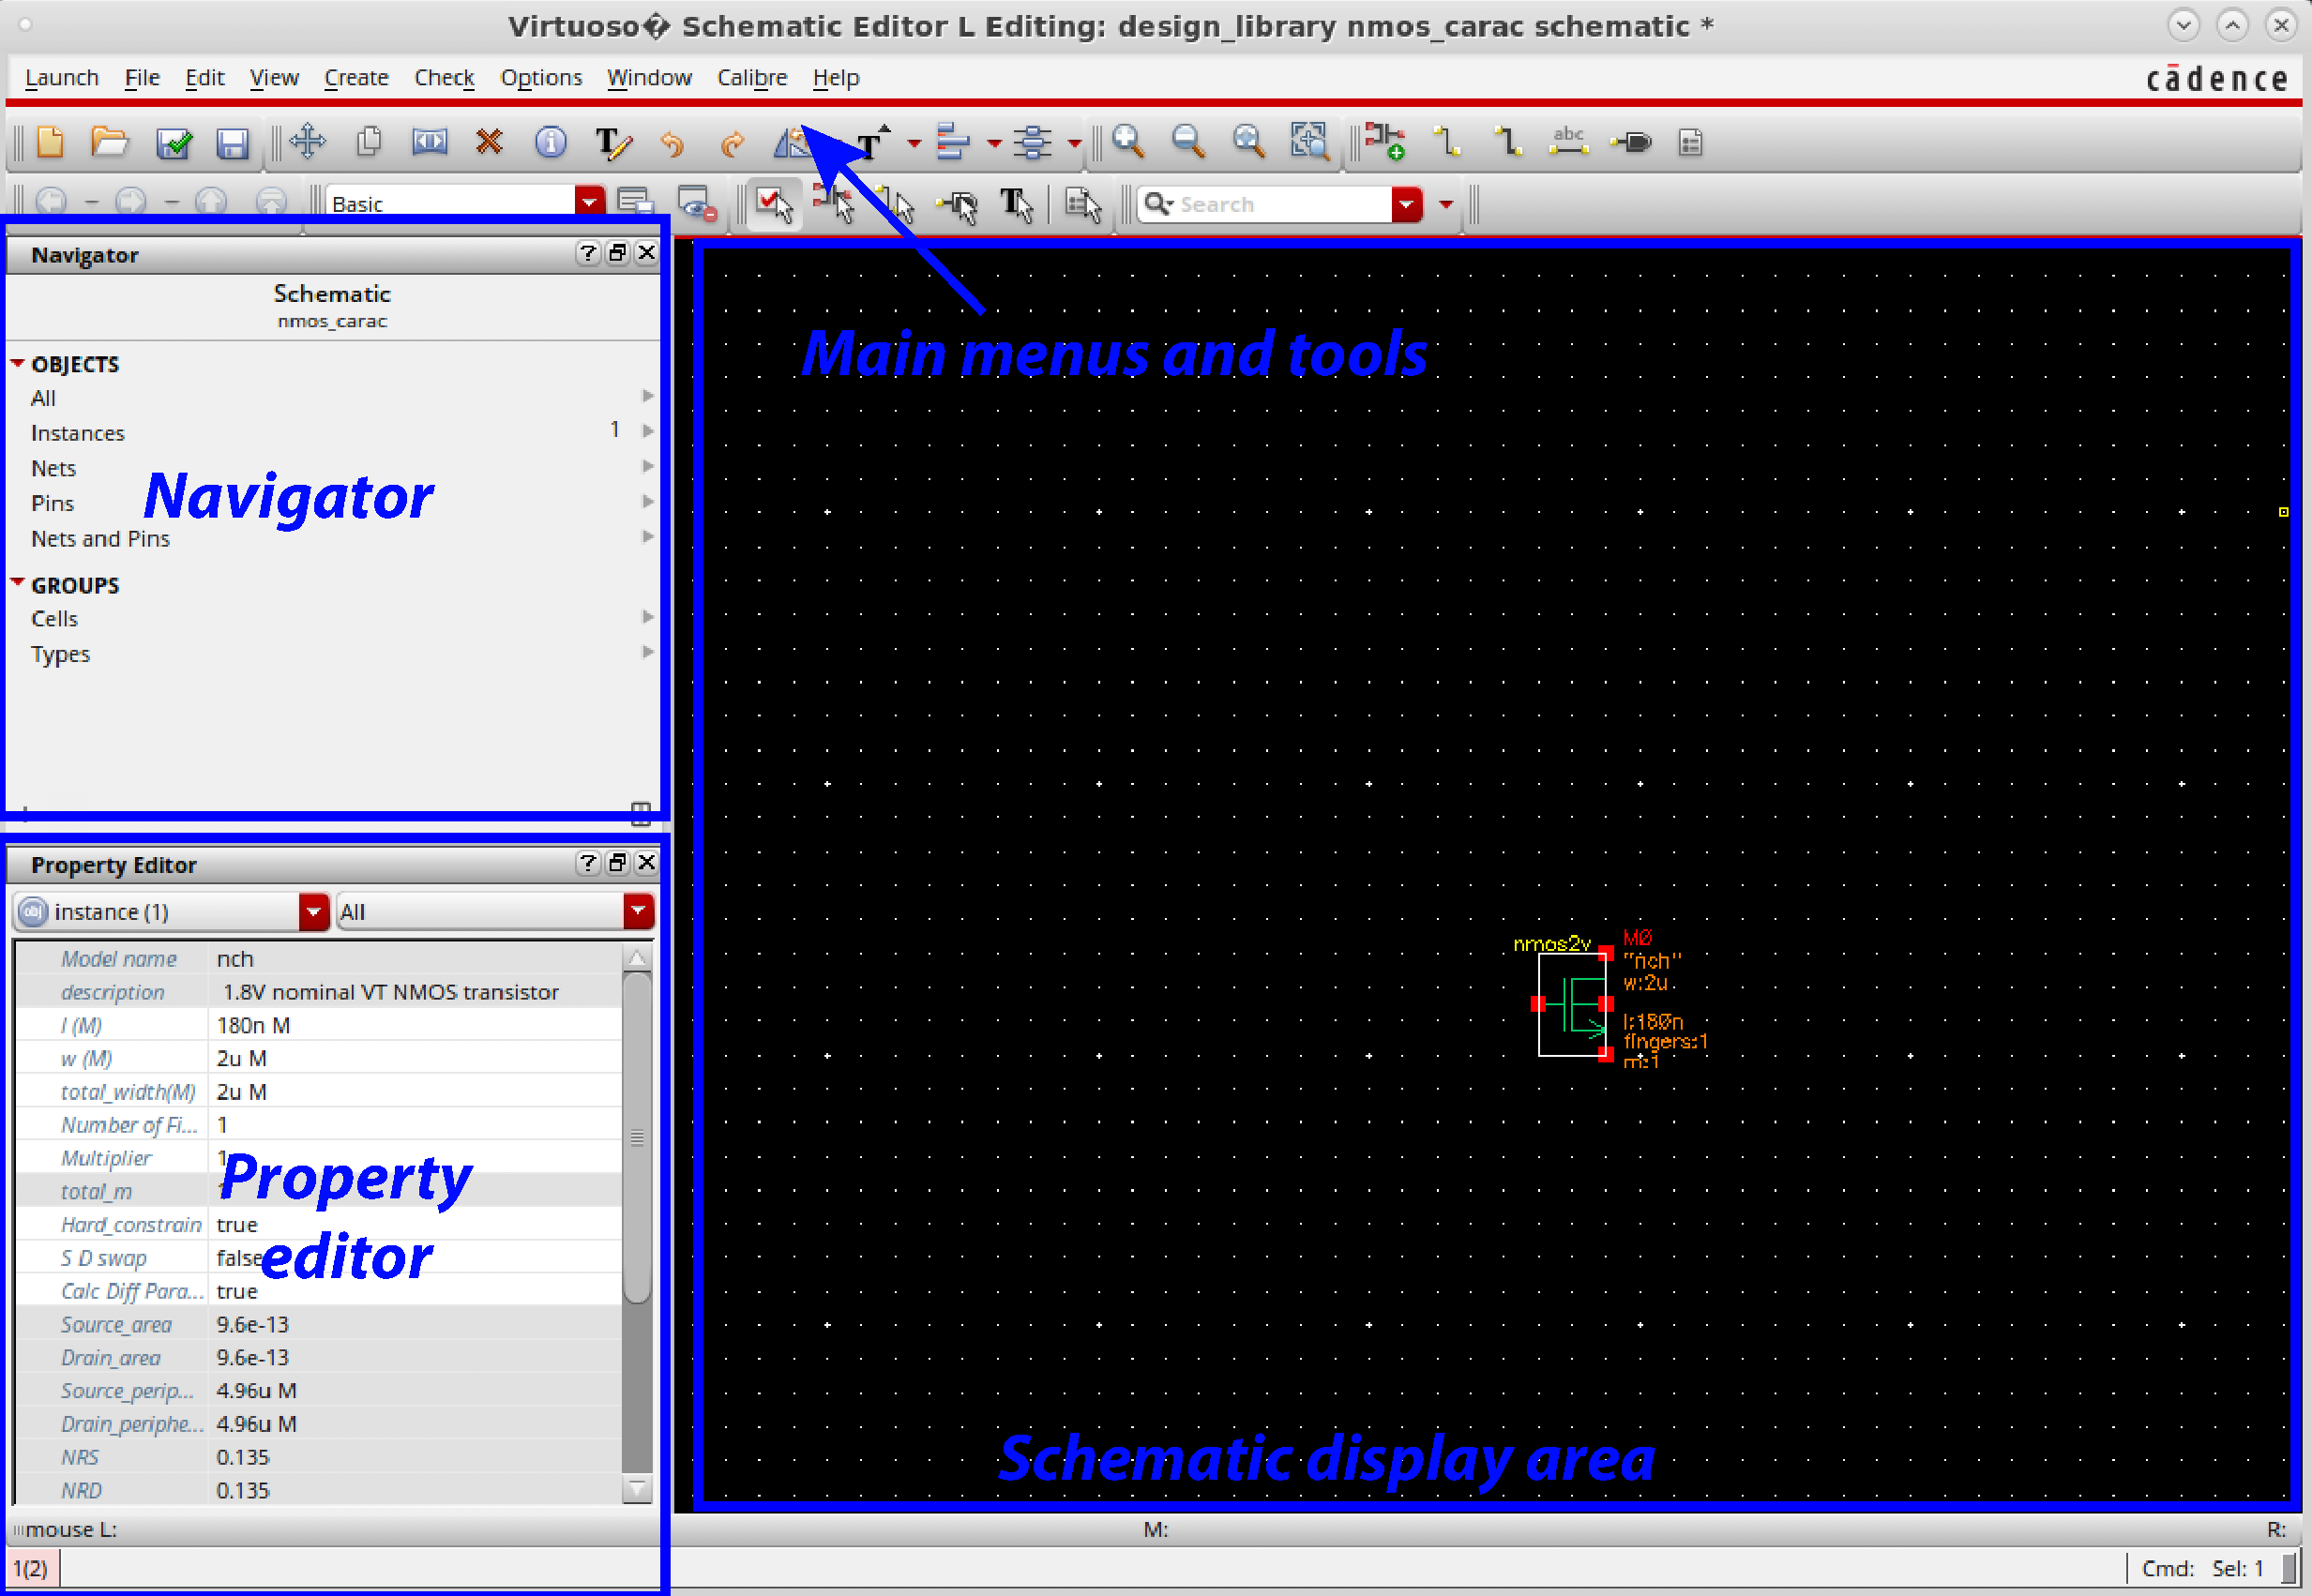
\includegraphics[scale=0.32]{figures/lab1_schematic_sim/schematicL.pdf}
		\caption{Schematic editor L window.}
		\label{fig_schematicL}
	\end{figure}
	
	
	\parbox[t]{\dimexpr\textwidth-\leftmargin}{%
		\begin{wrapfigure}[22]{r}{0.4\textwidth}
			\vspace{-0mm}
			\centering
			\vspace{-\baselineskip}
			\includegraphics[scale=0.35]{figures/lab1_schematic_sim/instanciate}
			\caption{Component instantiation window.}
			\label{fig_instantiate}
		\end{wrapfigure}
		
		\item First, instantiate (\textit{Create -> Instance...} or press \textbf{i}) an $nmos$ transistor (\textit{$nfet$} from the \textit{$s8phis$\_$10r$} library), as shown in \ref{fig_instantiate}. $nfet$ and $pfet$ are the regular 1.8V $nmos$ and $pmos$ transistors you will use for all your designs in the remaining of the labs.
		\item Try to move your transistor on the display area to get more familiar with the tool. To do so, press \textbf{m}, click one the transistor and move it across the display area. Click again to place it where you want.
		\item Check the transistor width. To do so, click on the transistor and press \textbf{q} (or click on the transistor and modify its width directly through the property editor as explained earlier). From the window, you can modify it width, length, number of fingers, \textit{etc.}. Set the Model Name to nshort, and check that its width is $420nm$ ($.42um$). This is the smallest size given by default with the Skywater PDK. For the rest of the labs, you will generally use this size for transistors (but also take into account the fact that $pmos$ transistors have to be larger than $nmos$ and you also need to size your transistors accordingly when transistors are in series).\newline } 
	
	\parbox[t]{\dimexpr\textwidth-\leftmargin}{%
		\begin{wrapfigure}[7]{r}{0.5\textwidth}
			\vspace{-0mm}
			\centering
			\vspace{-\baselineskip}
			\includegraphics[scale=0.5]{figures/lab1_schematic_sim/paramdc}
			\caption{DC source parameter setup.}
			\label{fig_paramdc}
		\end{wrapfigure}
		\item Instantiate two voltage DC sources (\textit{vdc} from the \textit{analogLib} library) and place them in your design. One will be used to provide the gate voltage and the other one will be used for the drain voltage so place them near those terminals.
		\item Connect the voltage sources correctly to the drain and gate of your transistor. To do so, you need to create some wires to connect the different parts of your circuit ((\textit{Create -> Wire (Narrow)} or press \textbf{w}) and join the two points you want to connect.\newline } 
	
	\begin{remark}
		After pressing \textbf{w} to create a wire, you can press \textbf{s} (snap) so the wire will automatically connect to the closest pin from your mouse.
	\end{remark}
	
	\item Connect the bottom pin of your voltage sources to the ground. You need to use the \textit{gnd} instance from the \textit{analogLib} library.
	\item In the same manner, connect the source of your $nmos$ to the ground. Do not forget to connect the bulk to the ground as well since you are using an $nmos$.
	
	
	
	\parbox[t]{\dimexpr\textwidth-\leftmargin}{%
		\begin{wrapfigure}[12]{r}{0.3\textwidth}
			\vspace{-0mm}
			\centering
			\vspace{-\baselineskip}
			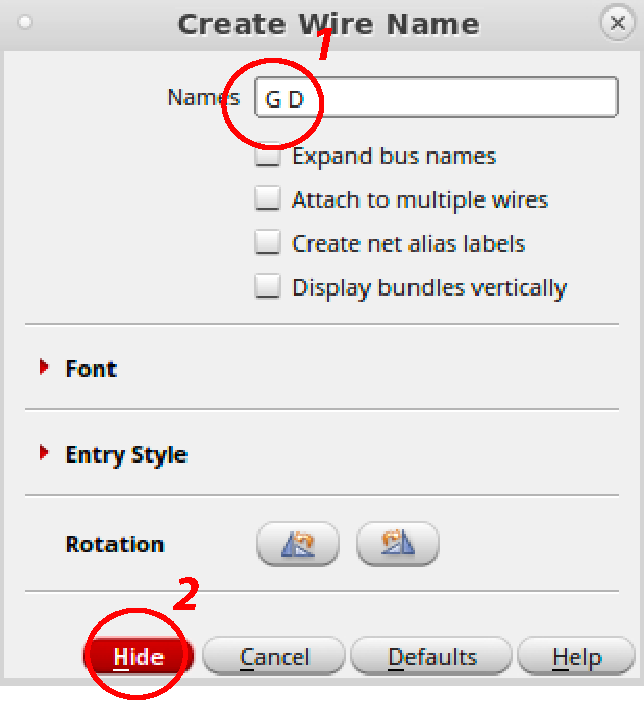
\includegraphics[scale=0.4]{figures/lab1_schematic_sim/label.pdf}
			\caption{Label creation.}
			\label{fig_label}
		\end{wrapfigure}
		\item Edit each of your voltage sources (click on it and press \textbf{q}) to specify the DC voltage as a variable as shown in Fig. \ref{fig_paramdc}. In that way, the voltage of your sources are defined as global variables and you will be able to directly modify them later in your simulation. 
		\item Create some labels for the important wires (in this case, the drain D and gate G of your transistor). All the connected wires are electrically at the same potential and together define a \textbf{net}. It will also help you to know which curve is what when doing the simulation (otherwise the names are assigned randomly). To do so, \textit{Create -> Wire Name...} or press \textbf{l}. Then specify the name(s) of the wire(s) you want to label and click Ok, as depicted in Fig. \ref{fig_label}. Then, click on the respective wire(s) you want to label from your schematic.\newline } 
	
	\parbox[t]{\dimexpr\textwidth-\leftmargin}{%
		\begin{wrapfigure}[12]{r}{0.6\textwidth}
			\vspace{-0mm}
			\centering
			\vspace{-\baselineskip}
			\includegraphics[scale=0.6]{figures/lab1_schematic_sim/nmos_carac}
			\caption{$nmos$ transistor testbench schematic.}
			\label{fig_nmos_carac}
		\end{wrapfigure}
		\item Check and Save your schematic (\textit{File -> Check and Save} or \textbf{Shift + X}). The schematic will be checked for potential errors. If there are any errors or warnings, a dialog box will inform you about them and the CIW will display a detailed message for each problem found.
		\item Your schematic should look like Fig. \ref{fig_nmos_carac}.\newline } 
	
	
\end{enumerate}
\newpage
\subsubsection{Performing the Simulation}
\begin{enumerate}
	\parbox[t]{\dimexpr\textwidth-\leftmargin}{%
		\begin{wrapfigure}[16]{r}{0.6\textwidth}
			\vspace{-0mm}
			\centering
			\vspace{-\baselineskip}
			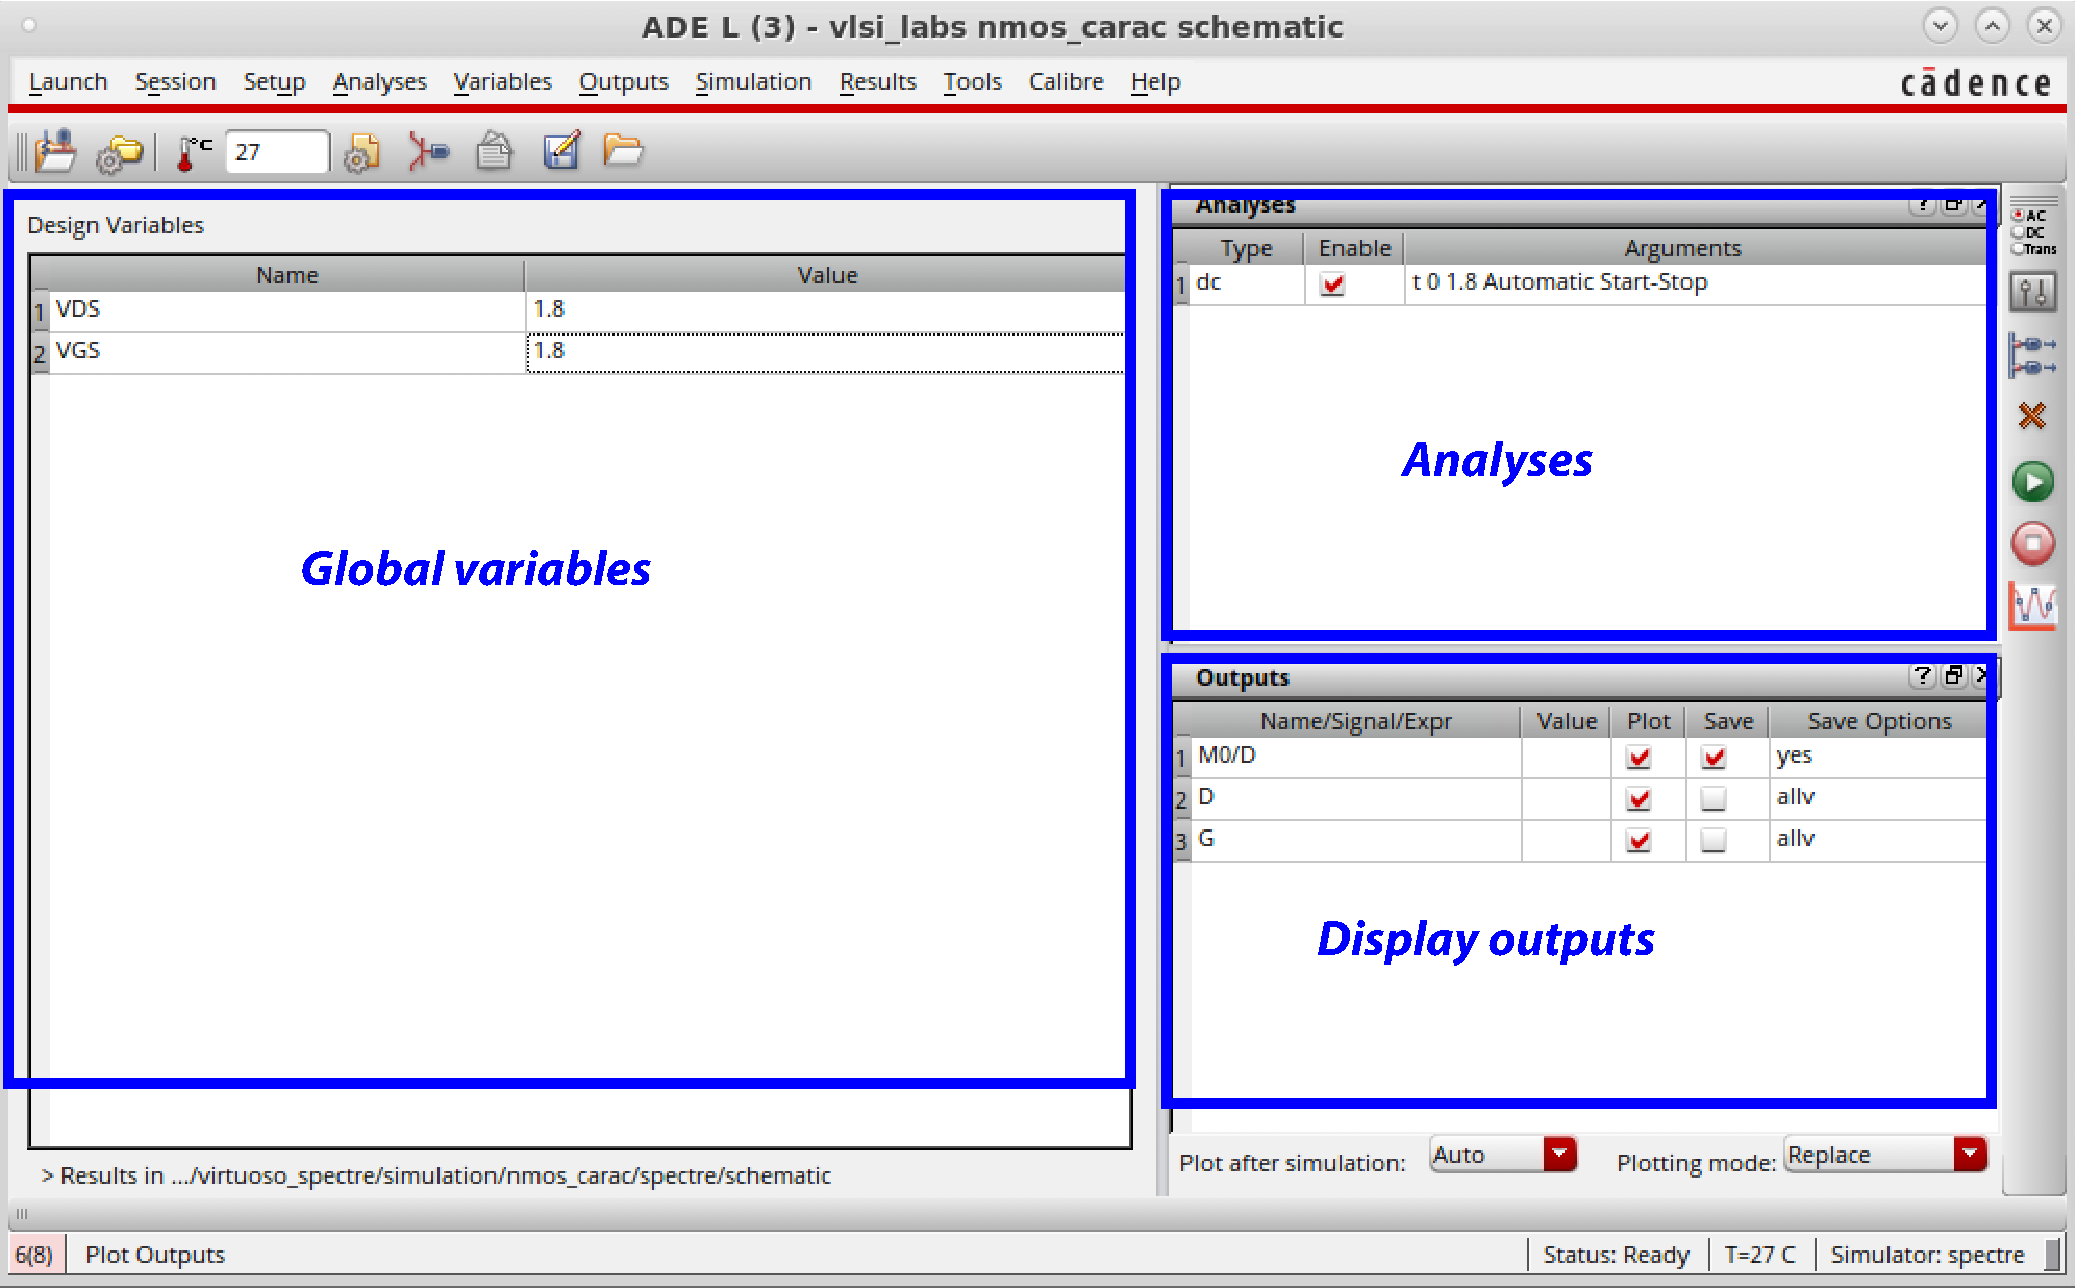
\includegraphics[scale=0.3]{figures/lab1_schematic_sim/ADE.pdf}
			\caption{ADE L window.}
			\label{fig_adel}
		\end{wrapfigure}
		\item Launch the simulation environment (\textit{Launch -> ADE L}). The ADE L window should appear (Fig. \ref{fig_adel}). The \textbf{\textcolor{blue}{Global variables}} is where all your design variables are defined (transistor width or length, source voltages, \textit{etc.}). Note that only the variables you define as a parameter in your schematic can be used as global variable. The \textbf{\textcolor{blue}{Analyses}} panel defines the different analyses you will run on your schematic (transient, DC, AC, \textit{etc.}). The \textbf{\textcolor{blue}{Display outputs}} is where you choose which output (voltage, current, parameter) will be displayed after the simulation.
		\newline } 
	
	
	\parbox[t]{\dimexpr\textwidth-\leftmargin}{%
		\begin{wrapfigure}[22]{r}{0.35\textwidth}
			\vspace{-0mm}
			\centering
			\vspace{-\baselineskip}
			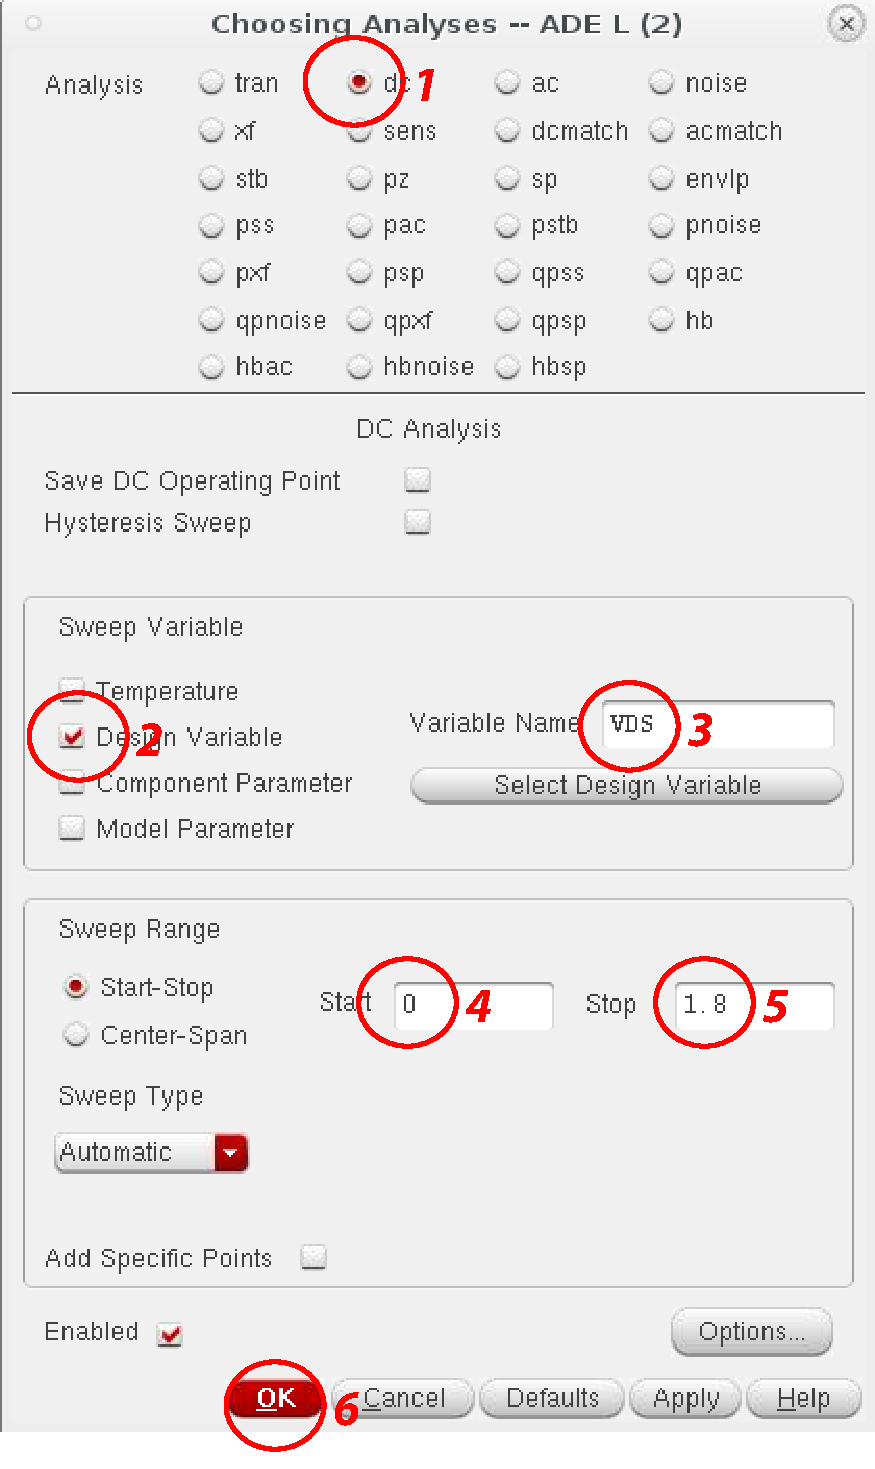
\includegraphics[scale=0.4]{figures/lab1_schematic_sim/dcsweep.pdf}
			\caption{DC sweep analysis.}
			\label{fig_dcsweep}
		\end{wrapfigure}
		\item First, you need to import your design variables (in this case the gate and drain source voltage you previously defined as parameters) to be able to define their value. To do so, go on the ADE window and do: \textit{Variables -> Copy from Cellview}. Don't forget to specify an initial value for your parameter in the left field, otherwise, the simulation will not run. In our case, we can set both voltages to the nominal supply voltage of this technology node: 1.8V.
		\begin{warning}
		In the ADE environment, when specifying a value (after importing your variable for instance, do not indicate their unit).
		\end{warning}
		\item Specify which kind of simulation you want to run. In this case, we are doing a DC simulation (\textit{Analyses -> Choose... -> dc}) and we want to draw an I-V curve so we need to sweep the drain voltage from $0$ to $1.8V$. To do so, you need to select the $design variable$ option, choose the variable name as $VDS$ and sweep if from $0$ to $1.8V$, as illustrated in Fig. \ref{fig_dcsweep}.
		\item Select which outputs you want to plot (\textit{Outputs -> To Be Plotted -> Select On Design}). The schematic window should appear. Select the gate and drain voltage as well as the drain current. Your ADE window should look like the one on Fig. \ref{fig_adel}.
		\begin{remark}
			When selecting which output to display for the ADE, you can select a voltage by clicking on the associated wire. To select a current, click on the associated terminal (red square on the schematic). 
	\end{remark}} 
	\item Run your simulation by clicking on the green triangle button and observe the I-V curve (Fig. \ref{fig_savestate} (a)).
	
	
	
	
	
	\begin{figure}[!h]
		\centering
		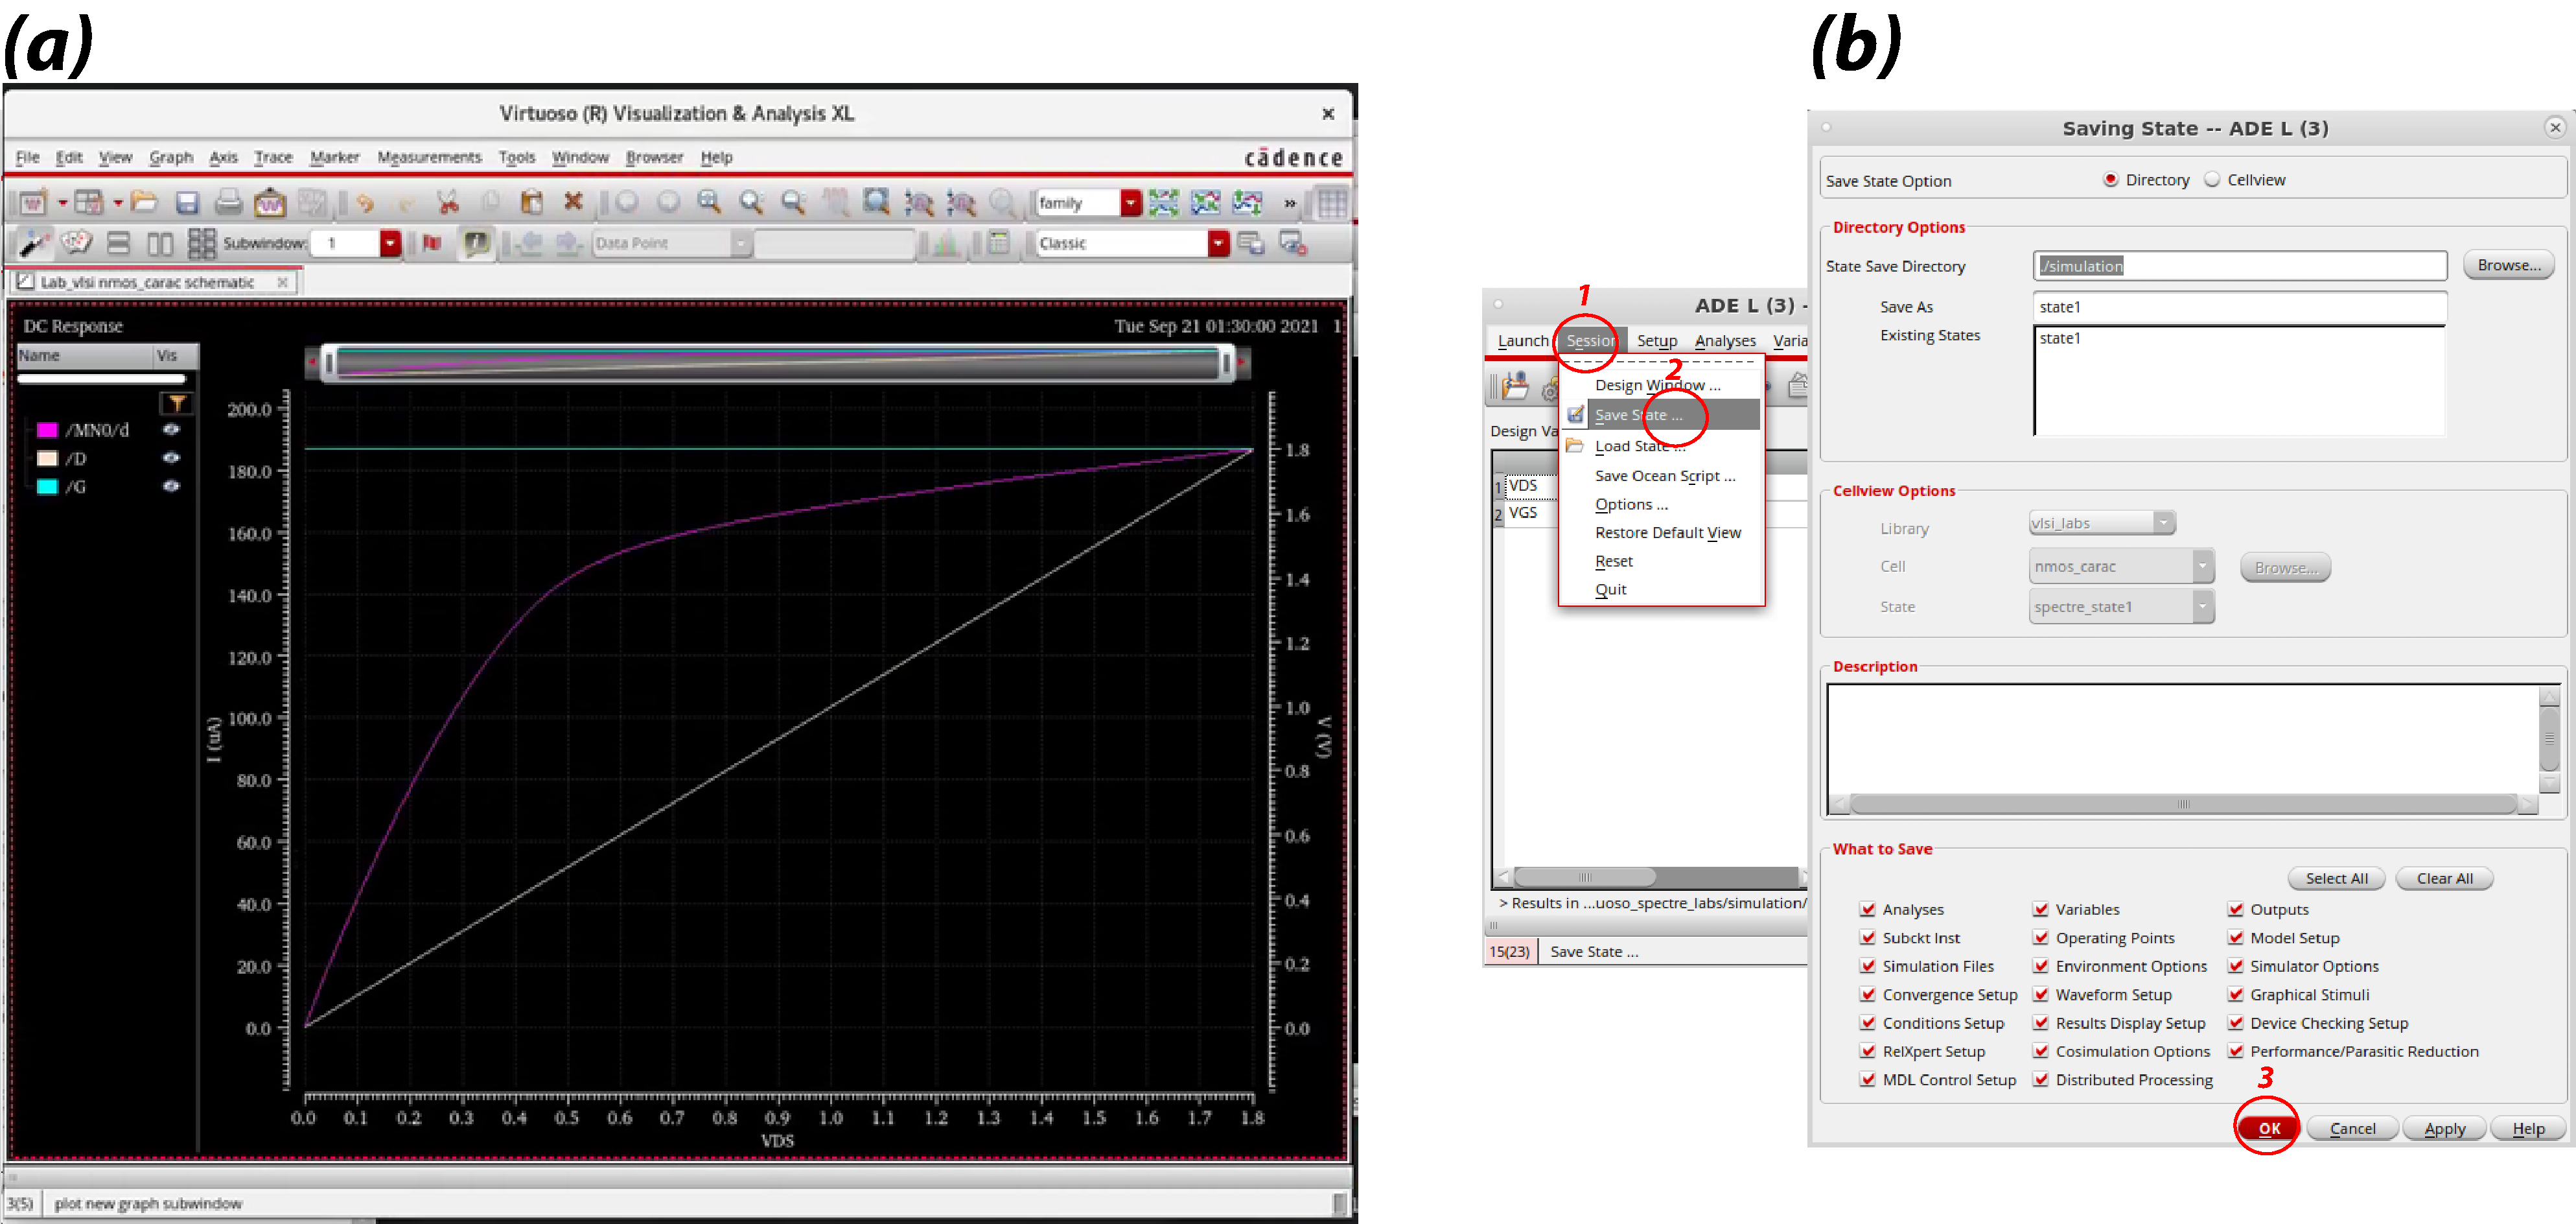
\includegraphics[scale=0.25]{figures/lab1_schematic_sim/save_state}
		\caption{(a) $nmos$ I-V curve; (b) Saving the ADE state.}
		\label{fig_savestate}
	\end{figure}
	
	
	\item Save your ADE L configuration so you can reopen it later without having to re-specify the displayed output signals, the analysis setup, the parameters, \textit{etc}. To do so: \textit{Session -> Save State... -> OK}, as shown in Fig. \ref{fig_savestate} (b).
	
	
	\begin{warning}
		For the rest of the lab, don't forget to save your ADE configuration for each testbench you do. 
	\end{warning}
	
	\item Now, plot the I-V curve for different $VGS$. To do so, you need to run a parametric DC analysis. A parametric analysis allows you to perform several simulations (transient, DC, \textit{etc}.) by sweeping a parameter. In case of a DC simulation, it allows you to sweep another parameter (you will sweep $VDS$ for different $VGS$). To run the parametric analysis, do as follows:
	\begin{enumerate}
		\item From the ADE L window, go to: \textit{Tools -> Parametric Analysis}. You can then choose which parameter to sweep as shown in Fig \ref{fig_paramsweep}. You can also choose the range and the number of steps. Here, you want to sweep $VGS$ from $0$ to $1.8V$ with 10 steps.
		
		\begin{figure}[!h]
			\centering
			\includegraphics[scale=0.6]{figures/lab1_schematic_sim/paramsweep}
			\caption{Parametric analysis setup for the DC sweep.}
			\label{fig_paramsweep}
		\end{figure}
		
		\item Run your simulation by clicking on the green triangle button from the parametric analysis window and observe the different I-V curves, as depicted in Fig. \ref{fig_paramcurve}.
		
		\begin{figure}[!h]
			\centering
			\includegraphics[scale=0.35]{figures/lab1_schematic_sim/parametric_curve}
			\caption{I-V curves for different \textit{VGS}.}
			\label{fig_paramcurve}
		\end{figure}
	\end{enumerate}
	
	
	\begin{exercise}\ \label{ex1}
		\vspace{-5mm}
		\begin{enumerate}
			\item Report the I-V curves under different $VGS$ voltages for your \textit {nmos} transistor.
			\item What are the $I_{on}$, $I_{off}$ of your $nmos$ transistor? Remember that $I_{on}$ is the maximum achievable current and $I_{off}$ if the current when $VDS$ is set to the supply voltage but when the gate is off ($V_{GS}=0V$).
		\end{enumerate}
	\vspace{-5mm}
	\end{exercise}	

\begin{checkpoint}\label{check1}
	Please call an assistant and show him that you obtained the I-V curves for different $VGS$ for your $nmos$ successfully.
\end{checkpoint}	
	
	\item Do the same exercise (create a new cell for it) to characterize a $pmos$ (\textit{$pfet$} from the \textit{$s8phis$\_$10r$} library) transistor. Do not forget that this time, the source of the $pmos$ has to be connected to $V_{DD}$ and that the $pmos$ is $on$ when $V_{GS}=0V$.
	
	\begin{exercise}\label{ex2}
Report the I-V curves under different $VGS$ voltages for your \textit {pmos} transistor as well as its $I_{on}$, $I_{off}$.
	\end{exercise}	
	
	
	\begin{remark}
		Don't forget that the power supply of this technology is $1.8V$. Also, don't forget to perform your I-V characterization for minimum sized $nmos$ and $pmos$ transistors.
	\end{remark}
\end{enumerate}	


\subsection{CMOS Inverter Simulation}
Now, you will create the schematic and symbol of a CMOS inverter. You will also perform some electrical simulations to study its transfer curve as well as its different delays.


\subsubsection{CMOS Inverter Schematic and Symbol Views}	
\begin{enumerate}
	\item Create a new schematic view in your design library for the CMOS inverter (\textit{File -> New -> Cellview...} from the Library Manager) and name it \textit{inv}.
	\item Instantiate two transistors (an $nmos$ and a $pmos$. Use regular transistors (\textit{$nfet$ and $pfet$} from the \textit{$s8phis$\_$10r$} library). The $nmos$ width should be set to $420nm$ (the minimum selectable for the nshort modelname). Set the width of the \textit{pmos} to 2 times the width of the \textit{nmos} (840nm).
	\item Create some wires as previously to connect the two transistors together, following the inverter schematic you saw in class. Don't forget to connect the source and the bulk of the $nmos$ together, as well as for the $pmos$.
	
	
	
	\parbox[t]{\dimexpr\textwidth-\leftmargin}{%
		\begin{wrapfigure}[30]{r}{0.4\textwidth}
			\vspace{-0mm}
			\centering
			\vspace{-\baselineskip}
			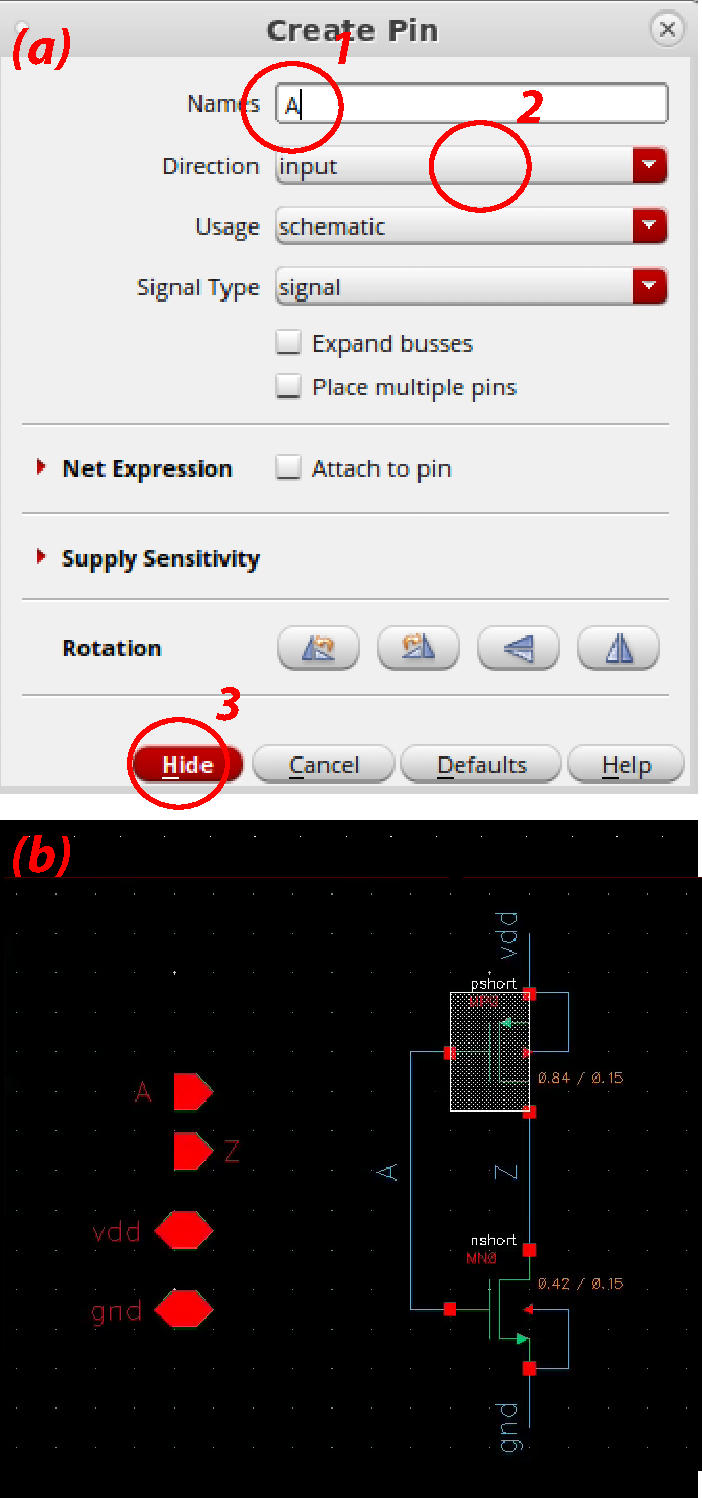
\includegraphics[scale=0.45]{figures/lab1_schematic_sim/pin_schematic.pdf}
			\caption{(a) Schematic pin creation; (b) CMOS inverter schematic.}
			\label{fig_pin}
		\end{wrapfigure}
		\item Create pins for your cell. Pins will define the different connections (interface) between a cell and its environment. If you instantiate a cell in other designs, the only accessible nets will be the previously defined pins. Pins are defined by the name and the direction (input, output or input-output). The purpose of the direction is to check for possible wrong connections (e.g. two outputs shorted together, or floating inputs). Typically, input-output pins are used for power supplies and bidirectional interfaces.
		
		\begin{itemize}
			\item Create the input pin. To do so: \textit{Create -> Pin} or press \textbf{p}. A window appears (Fig. \ref{fig_pin} (a), prompting you to enter the name ($A$) and the direction ($input$) of the pin. Click on \textit{Hide} and place the pin on the schematic. You can either place them directly on the net they are supposed to connect to, or on the left of your schematic (and connect the nets later through some labels).	
			\item Repeat the same process for the output (generally denoted \textit{Z}) and power supply pins ($V_{DD}$ and $G_{ND}$). Don't forget to specify the appropriate direction for each pin.
			\item Your schematic should look like Fig. \ref{fig_pin} (b). Don't forget to Check and Save your schematic and ensure there is no errors or warnings.
	\end{itemize}}
	
	
	\parbox[t]{\dimexpr\textwidth-\leftmargin}{%
		\begin{wrapfigure}[12]{r}{0.5\textwidth}
			\vspace{-0mm}
			\centering
			\vspace{-\baselineskip}
			\includegraphics[scale=0.4]{figures/lab1_schematic_sim/cellview}
			\caption{Cellview pin location.}
			\label{fig_cellview}
		\end{wrapfigure}
		\item Check and Save your schematic (\textit{File -> Check and Save} or \textbf{Shift + x}). Verify that there is no errors or warnings.
		\item Now, you will create a symbol for your inverter. A symbol is useful when you work with larger designs and you need to instantiate previously designed gates (e.g. designing an adder with some XOR and AND gates, \textit{etc.}), instead of redrawing the transistor schematic every time. The symbol will provide information on how to connect the cell from the outside. Note that the pins of your symbol should be the same ones defined in your schematic. To do so: 
		\begin{itemize}
			\item On the schematic window, (\textit{Create -> Cellview -> From Cellview..}). 
	\end{itemize} } 
	\begin{itemize}
		\item A window appears. All the options should be set correctly so just press OK.
		\item Another window appears (Fig. \ref{fig_cellview}) where you can specify the location of the pins on your symbol. It is a good practice to set the inputs on the left, the output on the right and the power supply pins on top or bottom, depending on the direction you chose when you defined your schematic pins, the pins should be correctly placed here.		
		\item Click OK.
		\item Shape your symbol how you want it, as depicted in Fig. \ref{fig_invsymbol} and Check and Save it. There should be no warnings or errors. 
		\begin{remark}
			You don’t need to change the $[$@instanceName$]$ and $[$@partName$]$ labels in the generated symbol. When you instantiate the cell, these labels will display the instance name and the cell name respectively. By default, the instances you place in a schematic will be named I0, I1, I2, \textit{etc}. To change the name of an instance, select the instance and press $Q$.
			
		\end{remark}
		
		\begin{figure}[!h]
			\centering
			\includegraphics[scale=0.45]{figures/lab1_schematic_sim/inv_symbol}
			\caption{Inverter symbol.}
			\label{fig_invsymbol}
		\end{figure}
	\end{itemize} 
	
\end{enumerate} 
\clearpage
\subsubsection{CMOS Inverter Testbench View}	
You previously created a schematic view of your inverter. However, this view only contains transistors. To perform electrical simulations on it, you need to create a view where you will instantiate some voltage sources, ground points, \textit{etc}. To do so, you need to create a new schematic cellview for your testbench in which you will instantiate your inverter.
\begin{enumerate}
	\item Go to the Library Manager and create a new schematic cellview ($inv\_testbench\_dc$ for instance). 
	\item Instantiate your inverter (you need to select the appropriate library and the inverter symbol cellview you just created) in your schematic.
	\item We will study the \textit{Voltage Transfer Characteristic} of the inverter so you first need to connect the input of your inverter to a DC source voltage ($vdc$ from the $analogLib$). Edit its property to specify the DC voltage as a parameter $VIN$.
	\item Instantiate another DC voltage source for the power supply. Set its DC voltage as a global parameter (VDD). 
	\item For the $V_{DD}$ and $G_{ND}$ symbols, use the $vdd$ and $gnd$ cells from the $analogLib$ library.
	\item For the load capacitor, use the $cap$ cell from the $analogLib$ library and sets its capacitance value to $10f F$.
	\item Don't forget to label your nets (input and output).
	\item Your testbench should look like Fig. \ref{fig_invtb}.
	
	\begin{figure}[!h]
		\centering
		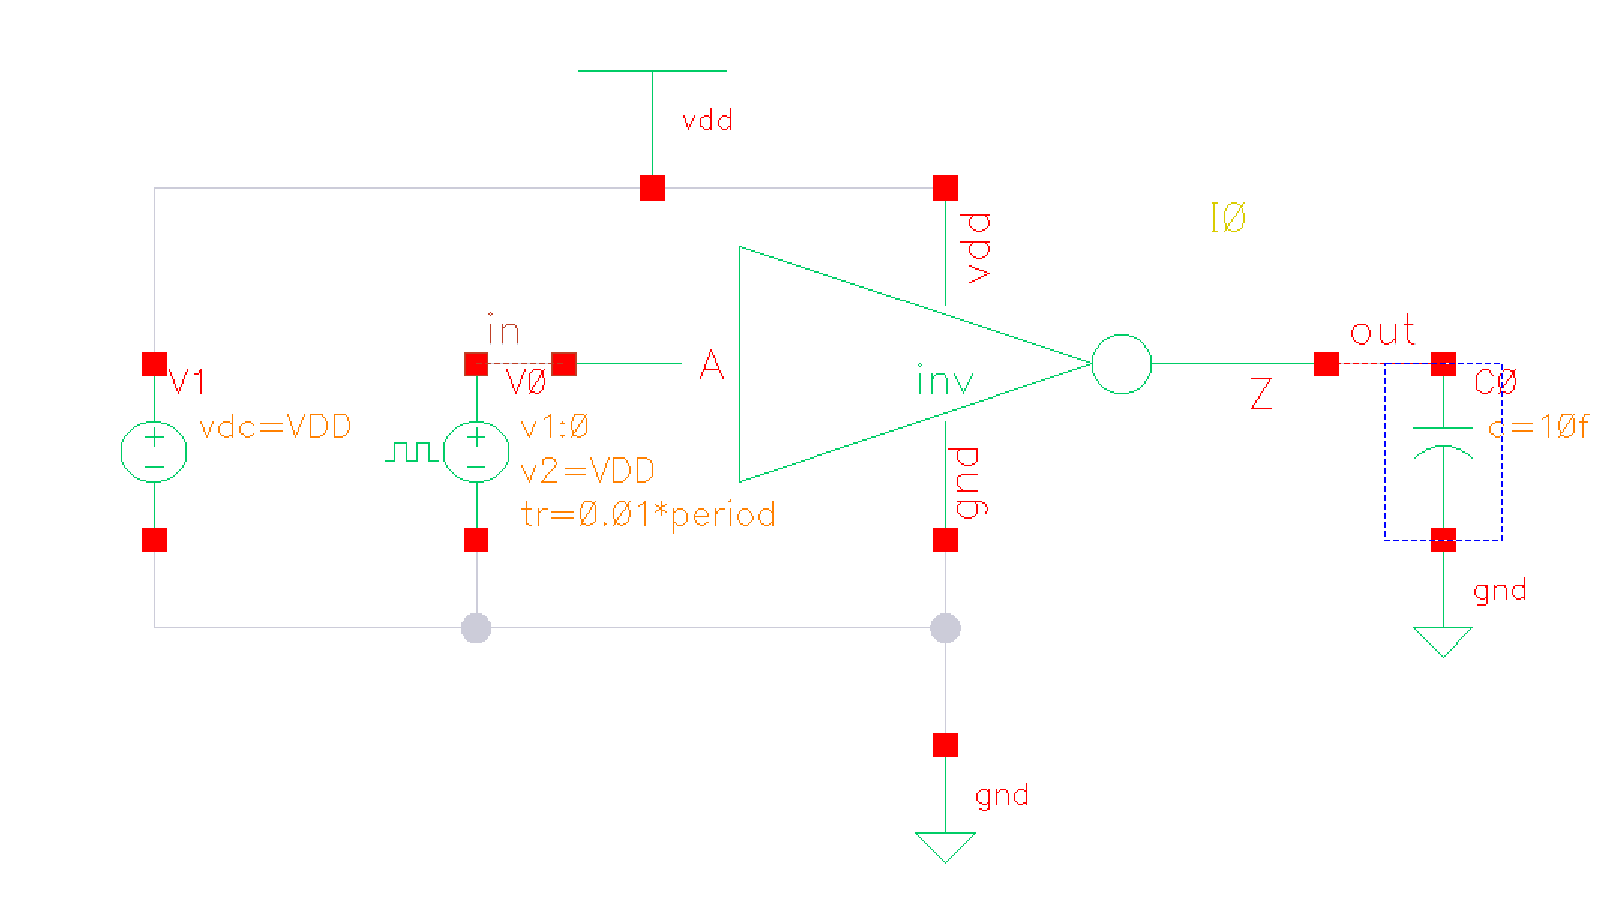
\includegraphics[scale=0.45]{figures/lab1_schematic_sim/inv_tb.pdf}
		\caption{Inverter testbench schematic.}
		\label{fig_invtb}
	\end{figure}
\end{enumerate} 
\begin{remark}
	At this point, you should have 2 cells: one for the inverter and one for the inverter testbench (in which the inverter is instantiated). For the rest of the labs, always create a different cell for your testbench and instantiate the standard cell you want to simulate in it.
\end{remark}
\subsubsection{CMOS Inverter DC Simulation}	
In this section, you will perform a DC simulation of an inverter in order to study the effect of the $pmos$ width on the VTC of your inverter.

\begin{enumerate} 
	\item Launch ADE L.
	\item Import your designs variables ($VIN$ and $VDD$) and set them to an initial value of 1.8V.
	\item Select the kind of analysis you want to run. In this case, you want to perform a DC sweep on $VIN$ going from 0V to 1.8V (the setup is really close to what you do previously for the $nmos$ characteristic).
	\item Select the signals to be displayed ($in$ and $out$ here).
	\item Run the simulation. Your curve should look like Fig. \ref{fig_vtc}.
	\begin{figure}[!h]
		\centering
		\includegraphics[scale=0.35]{figures/lab1_schematic_sim/vtc_curve}
		\caption{Inverter VTC curve.}
		\label{fig_vtc}
	\end{figure}
	
	\begin{exercise} \label{ex3}
		Plot the Voltage Transfer Curve (VTC), report the switching point of the inverter and specify the dimensions of your transistors.
	\end{exercise}	
	
	
	
	\parbox[t]{\dimexpr\textwidth-\leftmargin}{%
		\begin{wrapfigure}[9]{r}{0.5\textwidth}
			\vspace{-0mm}
			\centering
			\vspace{-\baselineskip}
			\includegraphics[scale=0.45]{figures/lab1_schematic_sim/width}
			\caption{Setting the transistor width as a parameter.}
			\label{fig_width}
		\end{wrapfigure}
		\item Run a parametric DC analysis for different width of the \textit{pmos} by sweeping the voltage from $0$V to $V_{DD}$. To do so:
		\begin{itemize} 
			\item Go to your inverter cell. To do so, you can either go to the library manager and open the inverter cell directly, or you can directly double click on the inverter symbol from your testbench schematic and click OK (in this case, you went down into the hierarchy. If you want to go back, press \textbf{ctrl + e}).\end{itemize} }
	\begin{itemize} 
		\item Change the width of the \textit{pmos} as a parameter and not a fixed number as shown in Fig \ref{fig_width}.
		\item On the ADE window, do: \textit{Variables -> Copy from Cellview} to import the new width variable on ADE. Don't forget to specify an initial value for your parameter in the left field (840nm for instance).
		\item Go to: \textit{Tools -> Parametric Analysis}. Specify the parameter to sweep as shown in Fig \ref{fig_param} (here \textit w is the width of the \textit{pmos}). 
		\item Run the simulation. \end{itemize} 
	
	
	
	\begin{figure}[!h]
		\centering
		\includegraphics[scale=0.55]{figures/lab1_schematic_sim/param}
		\caption{Parametric analysis setup.}
		\label{fig_param}
	\end{figure}
	
	
	\begin{exercise} \label{ex4}
		Plot the VTC curve for different width of the \textit{pmos}. What is this effect called? Report for which value of the \textit{pmos} width the switching point is equal to $V_{DD}/2$.
	\end{exercise}
	\item As you can see, the \textit{pmos} needs to be very big to have a switching point equals to $V_{DD}/2$. This leads to an unacceptable area and induces big parasitic capacitances. \textbf{For the rest of the labs, we will use the approximation $W_{pmos}=2*W_{nmos}$.}
	
	\begin{remark}
		In the next labs, don't forget to use the same approximation to size your transistors.
	\end{remark}
	\begin{warning}
		Don't forget to change the width value of the \textit{pmos} back to a fixed value (840nm). Otherwise, it will not be able to instantiate the transistor when creating a layout and to pass the LVS since the width will not be fixed.
	\end{warning}

\begin{checkpoint}\label{check2}
	Please call an assistant and show him that you obtained the VTC curve for your inverter successfully.
\end{checkpoint}	


\end{enumerate}

\subsubsection{CMOS Inverter Transient Simulation}	
In this part, we will perform another kind of simulation: transient simulation. It allows to study the behavior of your circuit overt time, when applying a specific input voltage sequence. Since the testbench will be slightly different, a good practice is to create a new testbench view for this particular simulation.
\begin{enumerate}
	
	\parbox[t]{\dimexpr\textwidth-\leftmargin}{%
		\begin{wrapfigure}[18]{r}{0.6\textwidth}
			\vspace{-0mm}
			\centering
			\vspace{-\baselineskip}
			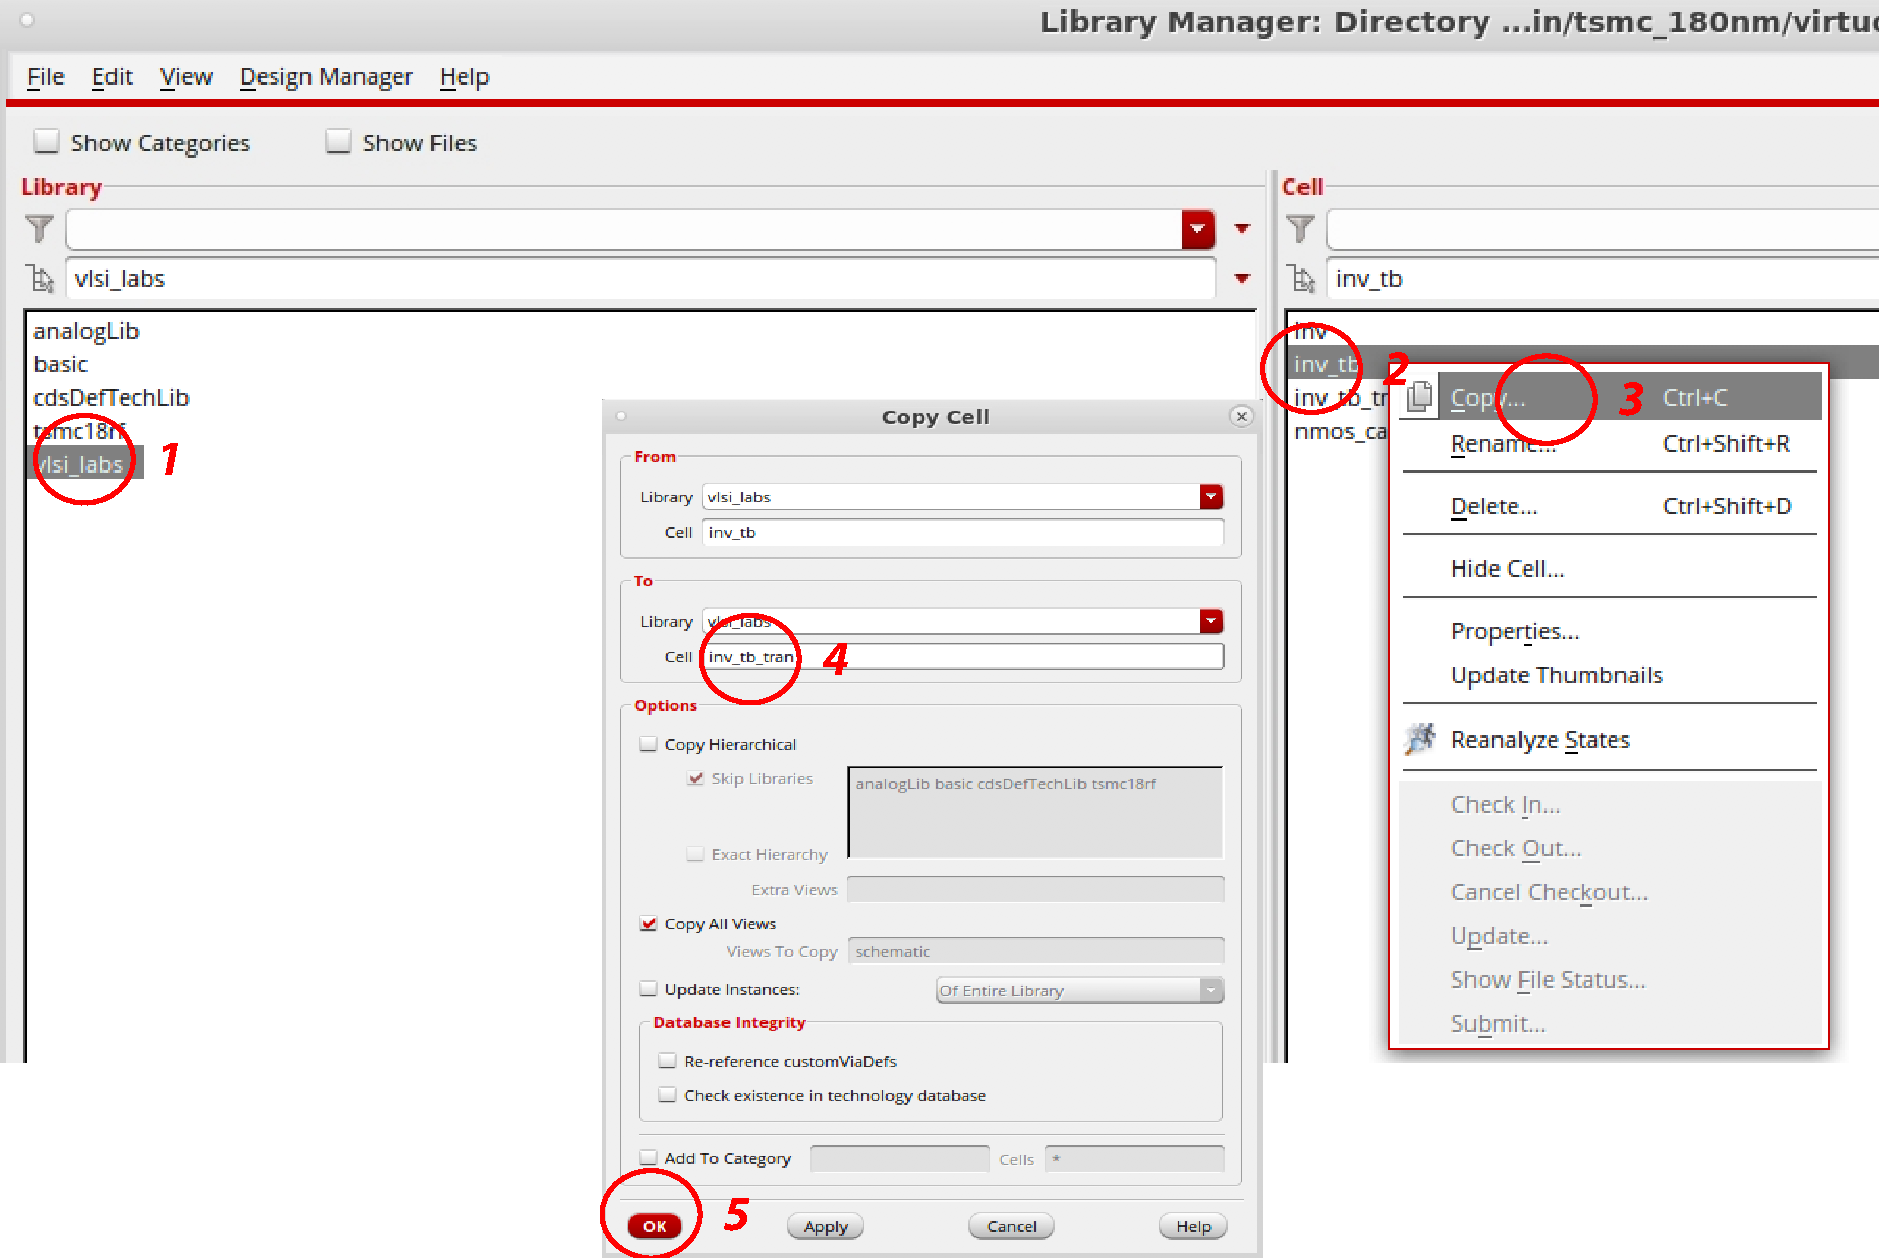
\includegraphics[scale=0.35]{figures/lab1_schematic_sim/copy.pdf}
			\caption{Copying a cell.}
			\label{fig_copy}
		\end{wrapfigure}
		\item First, create a new testbench for the transient simulation. Since the testbench is really similar to the DC simulation (only the input voltage source will change), an easy way to do is to copy the DC testbench and modify it. To do so:
		\begin{itemize}
			\item Go to the Library Manager, select your design library and your inverter testbench cell and right click and on and select $Copy...$.
			\item On the window, select the name you want ($inv\_testbench\_tran$ for instance) for this new testbench in the appropriate field and click OK (Fig. \ref{fig_copy}).
		\end{itemize}
	}
	\begin{itemize}
	\parbox[t]{\dimexpr\textwidth-\leftmargin}{%
	\begin{wrapfigure}[18]{r}{0.6\textwidth}
		\vspace{-0mm}
		\centering
		\vspace{-\baselineskip}
			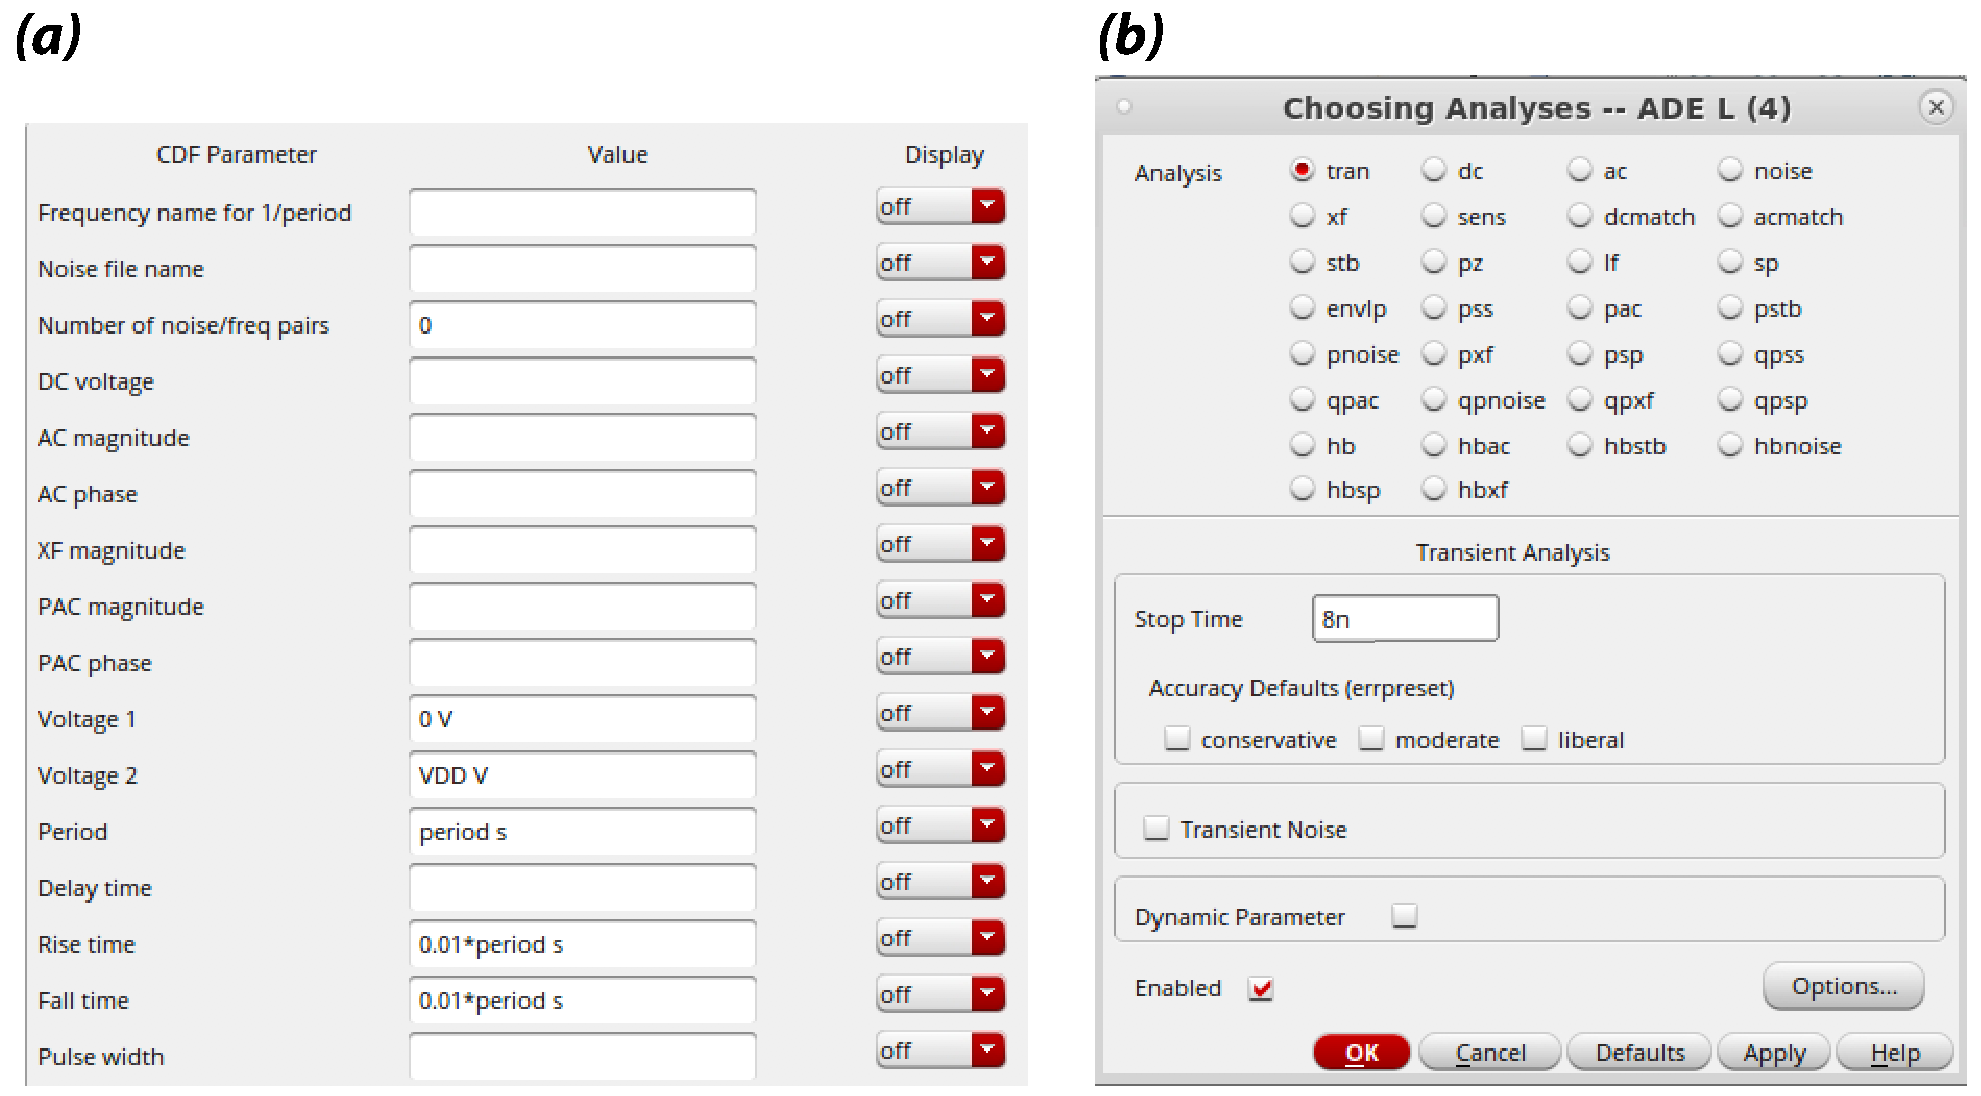
\includegraphics[scale=0.3]{figures/lab1_schematic_sim/tran_pulse}
\caption{(a) Transient simulation parameters; (b) Voltage pulse source parameters.}
\label{fig_pulse}
	\end{wrapfigure}
	\item Open the schematic cellview of your newly created testbench ($inv\_testbench\_dc$) and replace the input (not the supply one) source DC voltage by a pulse source $vpulse$ from the $analogLib$ library.
	\item Specify the parameters of your pulse source as shown in Fig. \ref{fig_pulse} (a). Note that this time, the DC voltage is specify as $Voltage 2$ and not as DC Voltage. Here, the period of your source is specified as a parameter $period$. You will be able to change this parameter in the ADE window later on. The rising and falling times depends on your period.
}
	\end{itemize}

	
	
	\parbox[t]{\dimexpr\textwidth-\leftmargin}{%
		\begin{wrapfigure}[22]{r}{0.5\textwidth}
			\vspace{-0mm}
			\centering
			\vspace{-\baselineskip}
			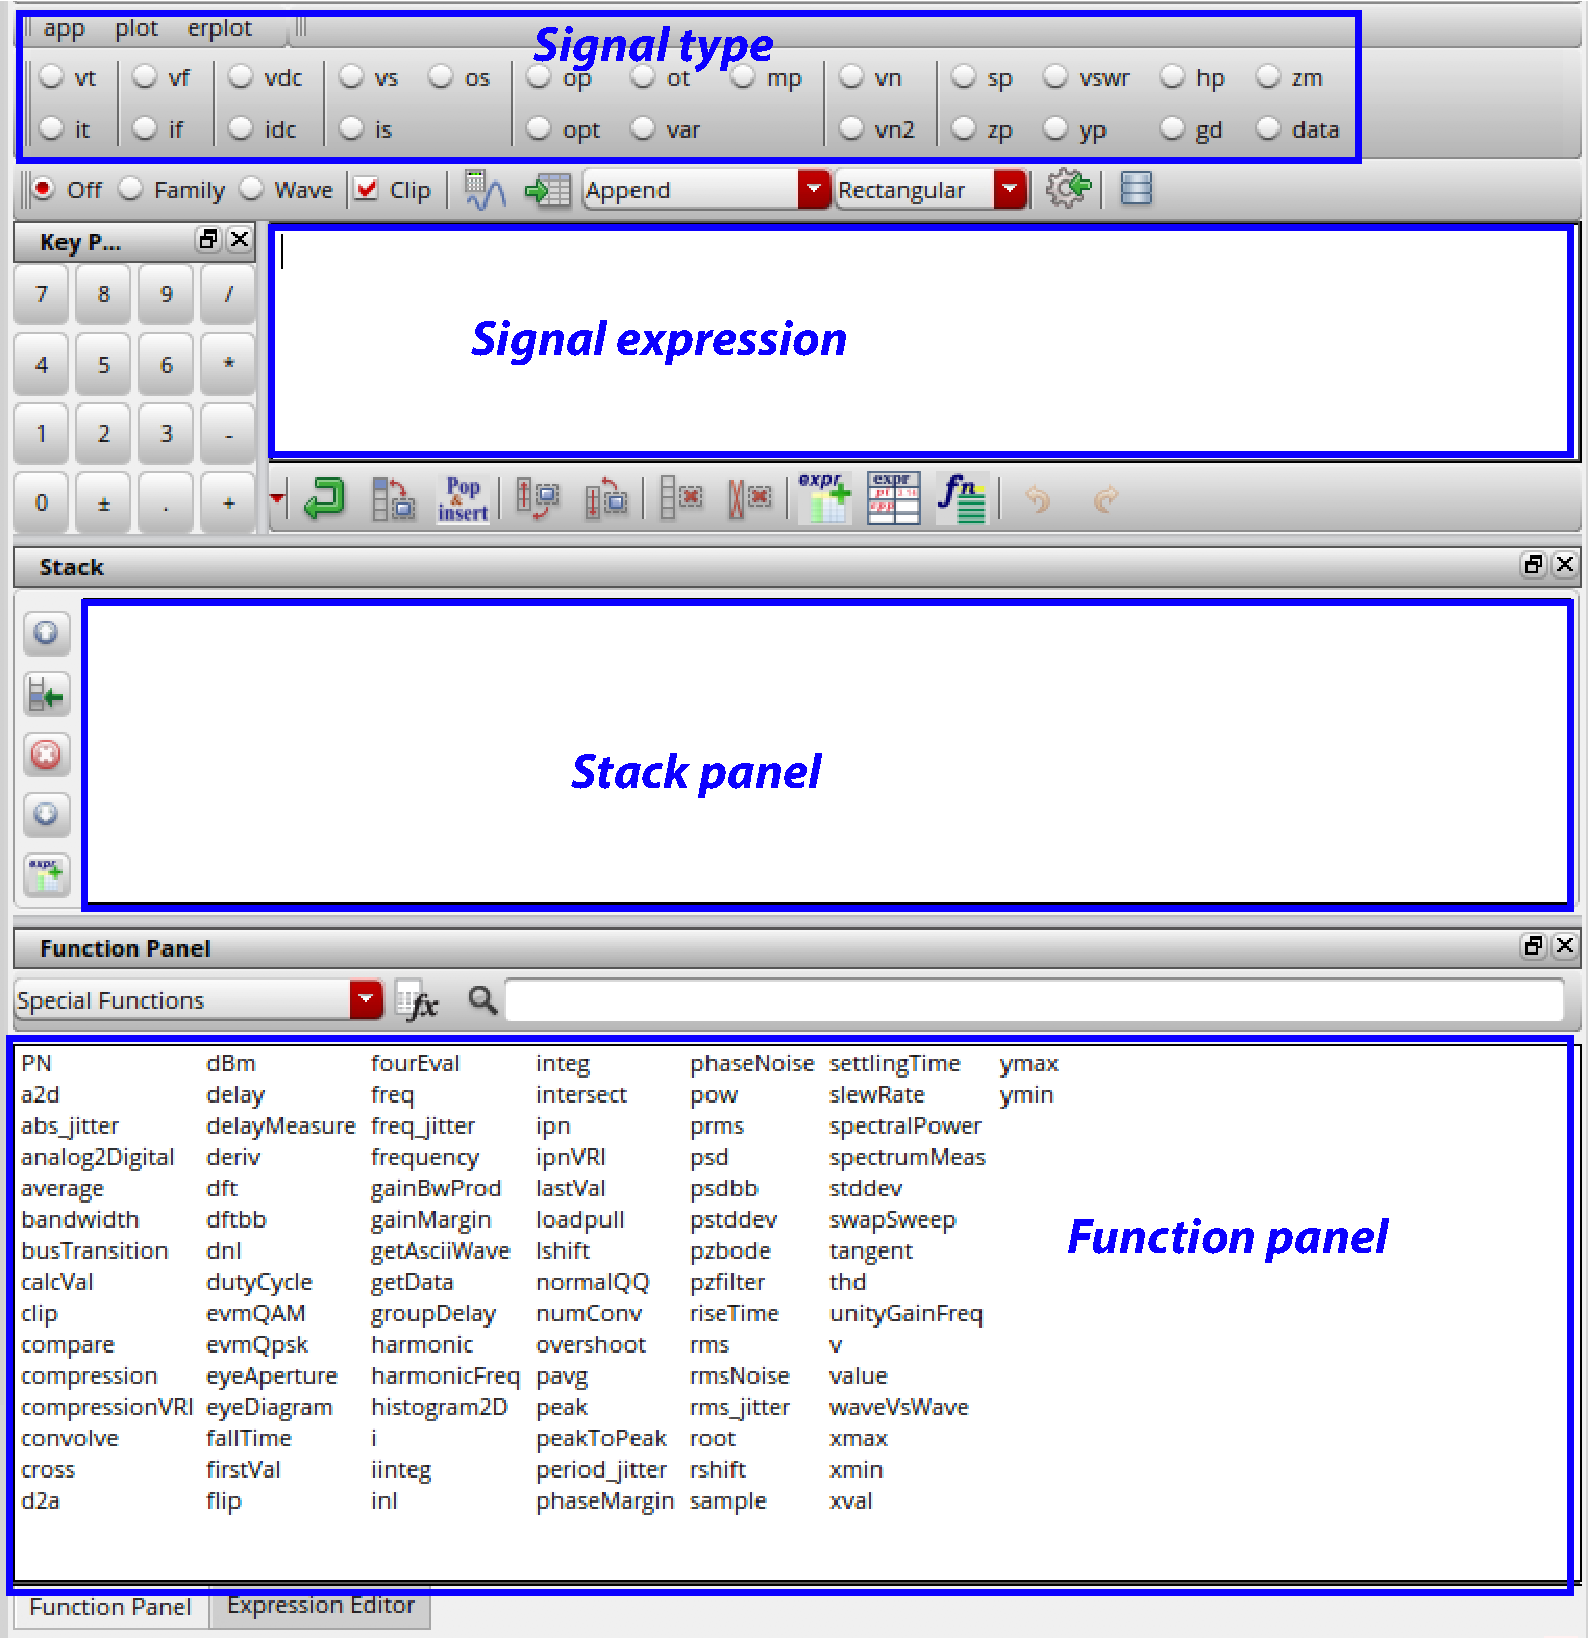
\includegraphics[scale=0.32]{figures/lab1_schematic_sim/calculator_tuto}
			\caption{ADE calculator setup.}
			\label{calculator}
		\end{wrapfigure}
		\item Launch ADE.
		\item Import your design variables and set some initial values. Use a period of 2ns.
		\item Specify a transient analysis (\textit{Analyses -> Choose... -> tran}) as shown in Fig. \ref{fig_pulse} (b) and just specify the stop time (8ns in this case in order to observe 4 period). 
		
		\item Define the delay measurements. To measure some stuff from the curves (falling time, propagation delay, maximum voltage etc.), we will use the Cadence calculator. To do so, first open the Calculator (in the ADE window: \textit{Tools -> Calculator...}).The calculator window should appear, as shown in Fig. \ref{calculator}. The Calculator is a very powerful tool which can help you define expressions and waveforms, plot circuit time or frequency responses, perform useful transforms, signal post-processing and/or analysis. It has many pre-defined mathematical and processing functions and also allows you to define your own functions. \newline
		The \textbf{\textcolor{blue}{Signal type}} panel allows you to choose which type of signal you want to consider (for instance, $vt$ stands for transient voltage). The \textbf{\textcolor{blue}{Signal expression}} panel which displays the expression of the signal you selected from your schematic through the \textbf{\textcolor{blue}{Signal type}} panel. Finally, the \textbf{\textcolor{blue}{Function panel}} allows you to choose which type of function you want to use (delay calculation, frequency response, \textit{etc}). 
	}
	
	\clearpage
	
	
			\item To compute the propagation delay:
	\begin{itemize}
		\parbox[t]{\dimexpr\textwidth-\leftmargin}{%
			\begin{wrapfigure}[21]{r}{0.6\textwidth}
				\vspace{-0mm}
				\centering
				\vspace{-\baselineskip}
				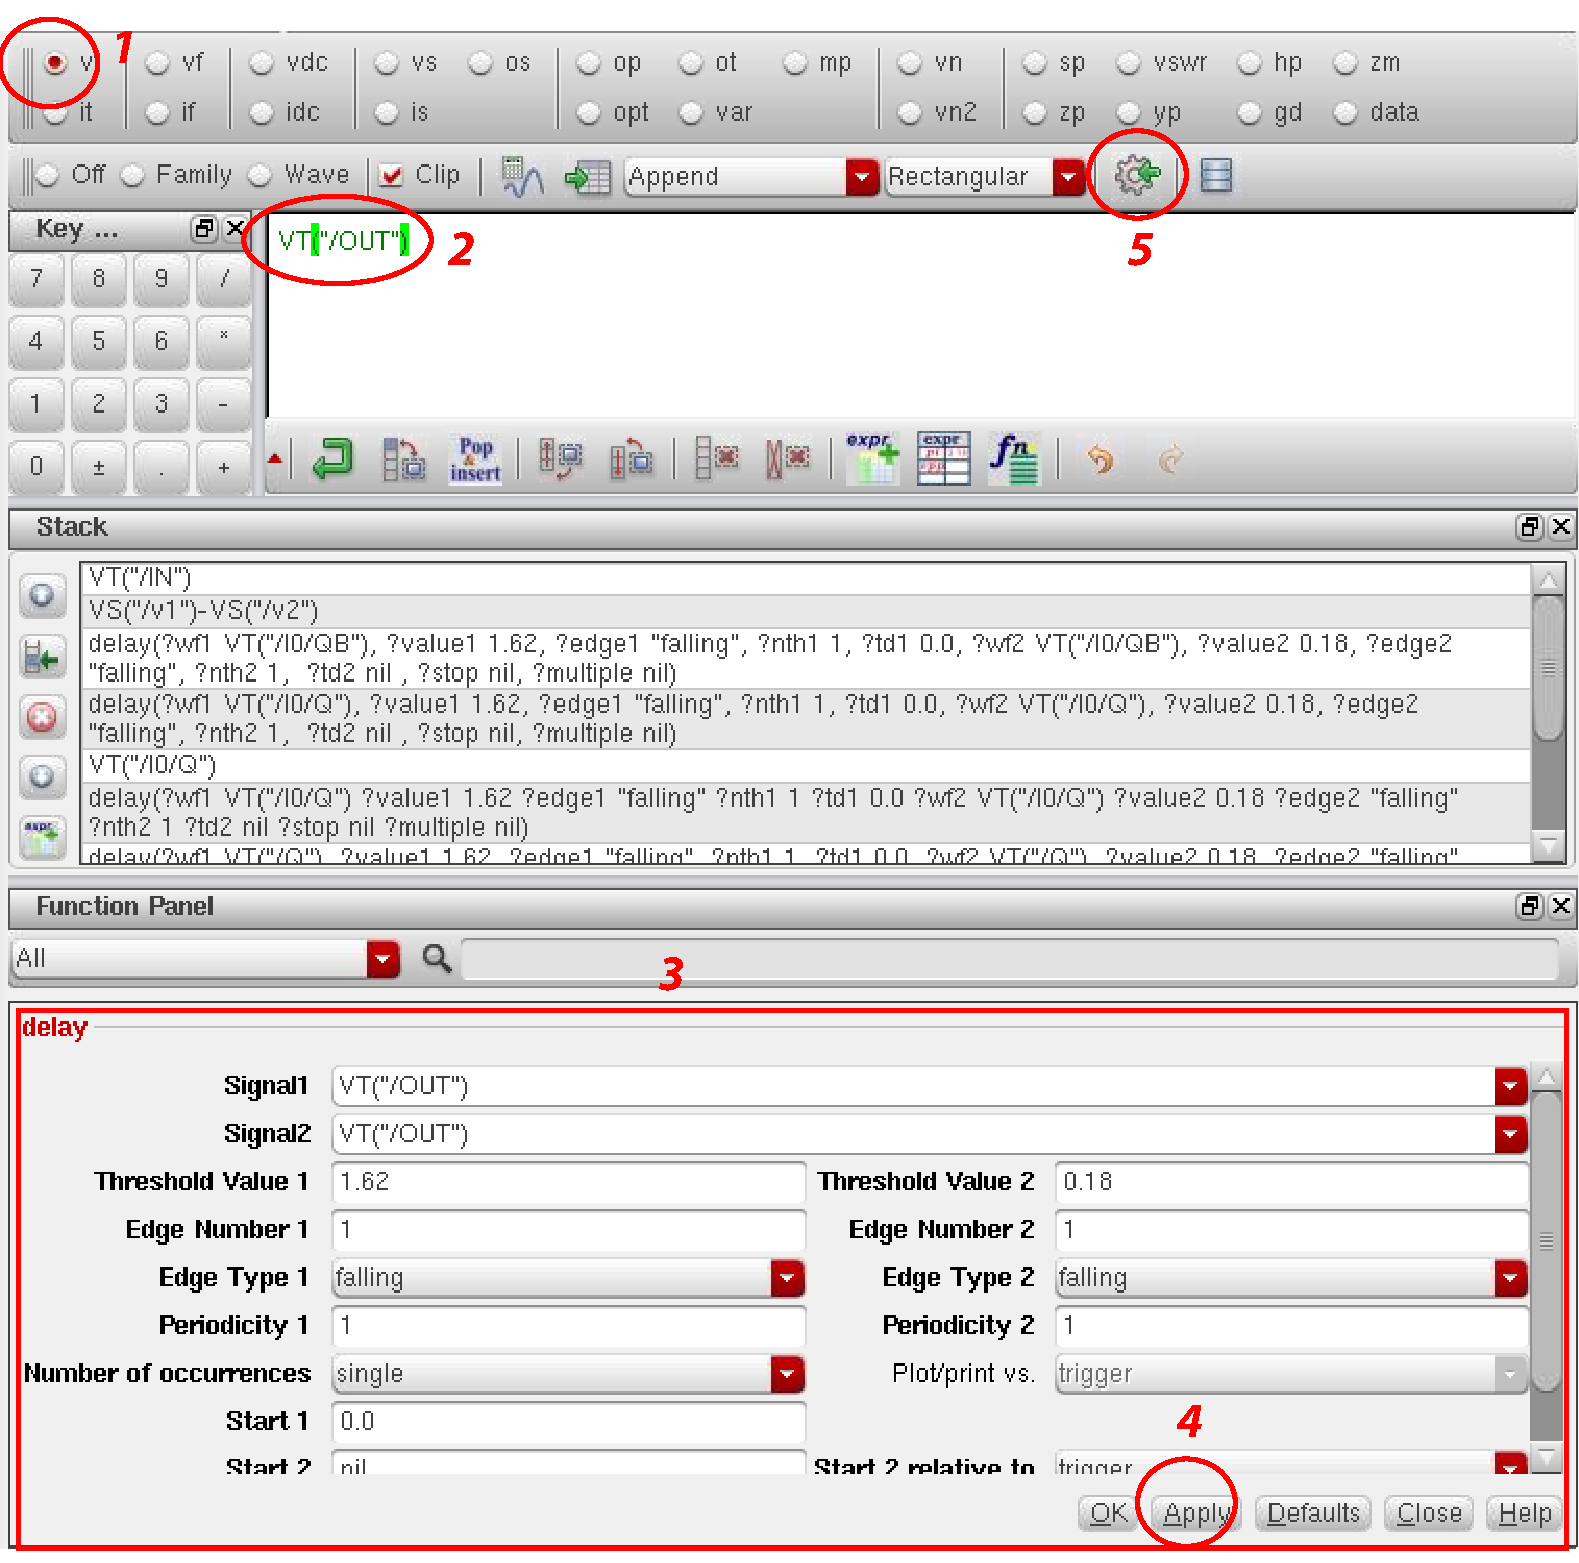
\includegraphics[scale=0.33]{figures/lab1_schematic_sim/calculator.pdf}
				\caption{ADE calculator setup.}
				\label{calculator}
			\end{wrapfigure}
			\item In the function panel, search for \textit{delay}.
			\item Select the appropriate signal you want to measure from (in this case, we want to measure the rising and falling time so select the output signal of your inverter): click on \textbf{vt} and select the signal on the schematic (step 1 in Fig. \ref{calculator}).
			\item Copy/paste the name of the signal in the Signal 1 and signal 2 fields of the calculator (step 2 in Fig. \ref{calculator}). Here, signal 1 and signal 2 are the same since we are measuring the falling delay which is on a single signal.
			\item Specify the other fields as in the picture (step 3 in Fig. \ref{calculator}). In this example, we show how to measure the falling delay (although the rising delay is obtained similarly). Threshold Value 1 is the value for which the time will be measured for the first point. If you want to measure the falling delay, it is $90\%$ of $V_{DD}$ so 1.62V. In the same manner, Threshold Value 2 is the value for which the time will be measured for the second point, so it is $10\%$ of $V_{DD}$ so 0.18V. Both Edge Types are falling since you are measuring a falling delay.		
					\item Click on \textit{Apply} (step 4).
			\item Finally, send the expression the ADE outputs (step 5). If you go back to the ADE window, the expression should be in the display output panel. Right click on it and select \textit{Edit} and change the \textit{Name (opt.)} field to an appropriate name (e.g. \textit{falling delay}).
			\item Redo the previous steps for the rising delay and the propagation delays. For the rising delay, note that both edges should be rising and the Threshold Values should be changed appropriately. For the propagation delay, don't forget to change Signal1 and Signal2 (this time, you are measuring a delay between the input and the output and not a delay on a single signal). Also, don't forget to carefully choose the threshold values (50$\%$) and the appropriate edge types.
		}
		
	\end{itemize}

\end{enumerate}

\begin{checkpoint}\label{check3}
	Please call an assistant and show him that you obtained the transient curve for your inverter successfully.
\end{checkpoint}	
\clearpage



\begin{exercise}\ \label{ex5}
	\vspace{-5mm}
	\begin{enumerate}
		\item Report the curve of the input/output of your inverter and the rising and falling times. Which one is faster? Why?
		\item Report the propagation delay of your inverter. How could you optimize it? At which cost?
		\item We considered a period time of 2ns. Is it slow, fast or appropriate compared to the frequency time of chips based on the 130$nm$ process? Justify your answer.			
	\end{enumerate}
\vspace{-5mm}
\end{exercise}


\subsection{Transient Simulation Under Different Process Corners}	
In VLSI design, corner simulations are used to represent the extreme cases of fabrication parameter variation and/or variation of other physical parameters such as the supply voltage or the temperature. When fabricated, depending on the fabrication process variations, devices may exhibit different behavior and therefore be faster, slower, larger, smaller and hence vary from the ideal case. As a result, the circuit may fall below the specifications. Corner simulations allow to model these cases and ensure that the circuit will still be functional under those variations. For your previous simulations, you used some model libraries in the \textit{tt} corner (typical $nmos$ - typical $pmos$) which are describing the characteristics (delay and power consumption mainly) of the transistors, diodes, \textit{etc.} under typical parameters. In this section, you will study the effect of the \textit{ss} (slow $nmos$ - slow $pmos$) and \textit{ff} (fast $nmos$ - fast $pmos$) corners on your design. To do so:	

\begin{itemize}
	\item From the ADE L window, click on \textit{Setup -> Model Libraries} as shown in Fig. \ref{fig_corner}.
	\item In the section column, find \textit{tt$\_$fet}, click on time on it, then a second time and change it to \textit{ff$\_$fet}.
	\item Run the simulation again and observe how the timing change.
	\item Repeat the process for the \textit{ss$\_$fet} corner.
	\begin{figure}[!h]
		\centering
		\includegraphics[scale=0.35]{figures/lab1_schematic_sim/tt}
		\caption{Changing the model library file corner.}
		\label{fig_corner}
	\end{figure}	
\end{itemize}

\begin{exercise}\ \label{ex6}
	\vspace{-5mm}
	\begin{enumerate}
			\item Report the rising and falling delays of your inverter for the \textit{ff} and \textit{ss} corners. How different are they from the \textit{tt} corner you used previously in the lab?
		\item After running some process corner simulations, if your inverter were to fall below a delay constraint, what could be done in order to make it faster and meet the constraint?
	\end{enumerate}
	\vspace{-5mm}
\end{exercise}

%process corner:
%Do with TT and SS
%what is the new delay? Why? If you had a timing constrain of XXX and it were failing for the SS corner, what could you do to ensure that your inv passes the specifications even for SS corner?

\section{Assignment and Checkpoint Summary}
Write a report and answer the assignments asked during the lab, which are summarized below. Do not forget to validate the checkpoints, summarized below as well, by an assistant before the end of the lab.


	\begin{exercisesum}\	
			\vspace{-2mm}
	\begin{enumerate}
		\item Report the I-V curves under different $VGS$ voltages for your \textit {nmos} transistor.
		\item What are the $I_{on}$, $I_{off}$ of your $nmos$ transistor? Remember that $I_{on}$ is the maximum achievable current and $I_{off}$ if the current when $VDS$ is set to the supply voltage but when the gate is off ($V_{GS}=0V$).
		\item Report the I-V curves under different $VGS$ voltages for your \textit {pmos} transistor as well as its $I_{on}$, $I_{off}$.
		\item Plot the Voltage Transfer Curve (VTC), report the switching point of the inverter and specify the dimensions of your transistors.
		\item Plot the VTC curve for different width of the \textit{pmos}. What is this effect called? Report for which value of the \textit{pmos} width the switching point is equal to $V_{DD}/2$.
		\item Report the curve of the input/output of your inverter and the rising and falling times. Which one is faster? Why?
	\item Report the propagation delay of your inverter. How could you optimize it? At which cost?
	\item We considered a period time of 2ns. Is it slow, fast or appropriate compared to the frequency time of chips based on the 130$nm$ process? Justify your answer.			
			\item Report the rising and falling delays of your inverter for the \textit{ff} and \textit{ss} corners. How different are they from the \textit{tt} corner you used previously in the lab?
	\item After running some process corner simulations, if your inverter were to fall below a delay constraint, what could be done in order to make it faster and meet the constraint?
	\end{enumerate}
\vspace{-5mm}
\end{exercisesum}	

\begin{checkpointsum}\
	\vspace{-2mm}
	\begin{enumerate}
		\item Please call an assistant and show him that you obtained the I-V curves for different $VGS$ for your $nmos$ successfully.
		\item Please call an assistant and show him that you obtained the VTC curve for your inverter successfully.
		\item Please call an assistant and show him that you obtained the transient curve for your inverter successfully.
	\end{enumerate}
	\vspace{-5mm}
\end{checkpointsum}
%\newcommand{\labtitle}{ECE/CS 5710/6710 - Lab 2}
%\newcommand{\labdate}{}
\newcommand{\labsubtitle}{CMOS Inverter - Physical Design}
\vlsiheader


\begin{center}
\LARGE\textbf{\labsubtitle} \\
	\large\textbf{Pre-lab Assignment:} Check for the date on Canvas. \\
	\large\textbf{Lab Report:} Check for the date on Canvas.
\end{center}
\section{Objectives}
The goal of this second lab is to teach you how to draw the layout of a CMOS inverter using the Skywater design kit. You will also learn how to verify your design through thse DRC and LVS steps and how to extract the layout parasitics for post-layout simulation purposes. For the DRC, LVS and PEX steps, you will use an industrial tool: Mentor Calibre\textsuperscript{\tiny\textregistered}.



\section{Pre-lab Assignment}
\begin{prelab}
Answer the following questions and submit a \textbf{.pdf} file through Canvas:
\begin{enumerate}
	\item What does DRC, LVS and PEX stand for? What are they used for?
	\item Draw the transistor schematic of a 2-input NAND gate and give its truth table.
	\item How are the transistor in a 2-input NAND gate usually sized? Justify your answer.
\end{enumerate}
	\vspace{-5mm}
\end{prelab}

\section{Introduction the the Tools}
In this lab, you will reuse Virtuoso\textsuperscript{\tiny\textregistered} for the layout as well as electrical simulations. You will also use Calibre\textsuperscript{\tiny\textregistered} is the suite for full-custom layout verification and parasitics extraction. Although it is coming from another vendor (Mentor, now part of Siemens), this tool is easily integrated into the Virtuoso\textsuperscript{\tiny\textregistered} environment.


\section{Lab Assignment}
\subsection{CMOS Inverter Layout Drawing}
In this part, you will learn how to draw the layout of the CMOS inverter. With this knowledge, you will then be able to draw the layout of more complex logic gates. To start this lab, launch Virtuoso\textsuperscript{\tiny\textregistered} from your \textit{virtuoso} subdirectory, as you did in the previous lab:
\begin{codeline}
	./start$\_$virtuoso.sh
\end{codeline}

\subsubsection{Layout Environment}
		\begin{remark}
	As explained in the previous lab, don't forget to check that in your inverter schematic view, the width of the $pmos$ is set to \textit{840nm} and not as a parameter, otherwise, you will have some issues when instantiating it in your layout.
\end{remark}
			\vspace{-8mm}
\begin{enumerate}
	
	\parbox[t]{\dimexpr\textwidth-\leftmargin}{%
		\begin{wrapfigure}[12]{r}{0.6\textwidth}
			\vspace{-0mm}
			\centering
			\vspace{-\baselineskip}
			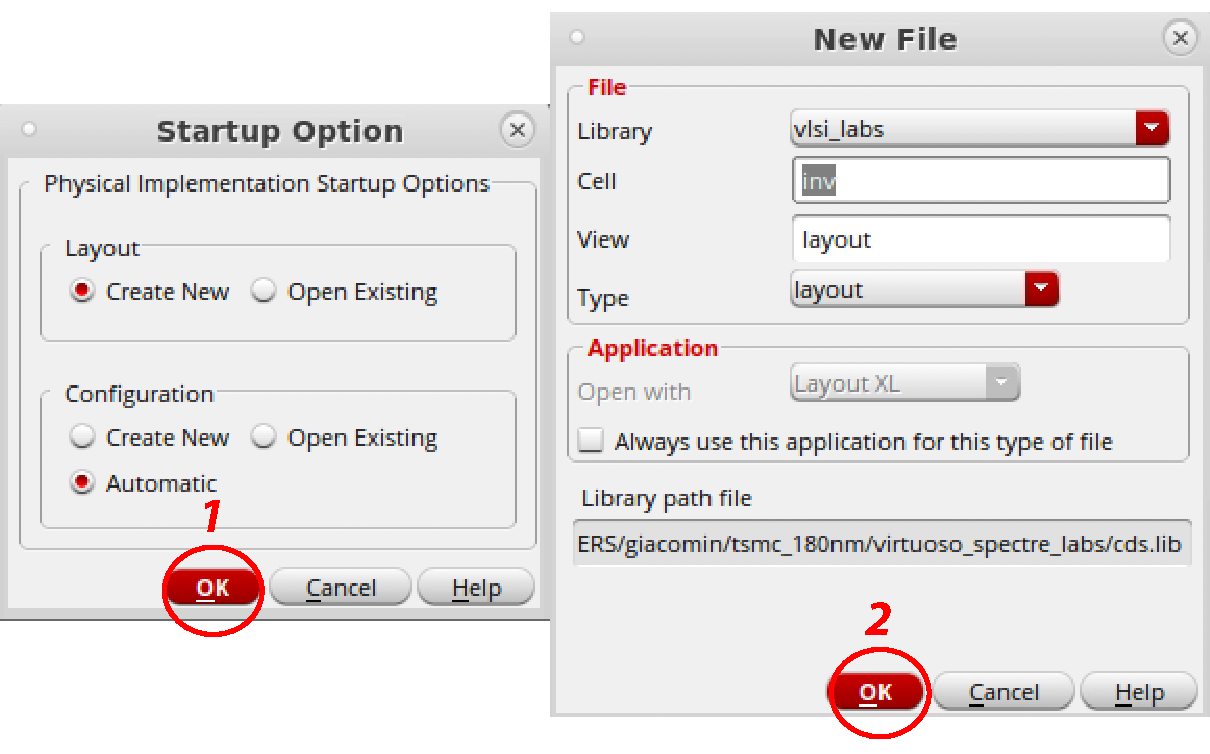
\includegraphics[scale=0.35]{figures/lab2_layout/layout_create.pdf}
			\caption{New layout view.}
			\label{fig_layoutfile}
		\end{wrapfigure}
		\item Create a new cellview for your inverter Layout. To do so, go to the open your inverter schematic and do: \textit{Launch - Layout XL ...}). Click OK on the first window. For the next window, select layout as the view name, and Layout XL as the desired application as indicated in Fig. \ref{fig_layoutfile} (the library and cell name will of course depend on what you chose earlier). \newline}
	
	
	\parbox[t]{\dimexpr\textwidth-\leftmargin}{%
		\begin{wrapfigure}[19]{r}{0.65\textwidth}
			\vspace{-0mm}
			\centering
			\vspace{-\baselineskip}
			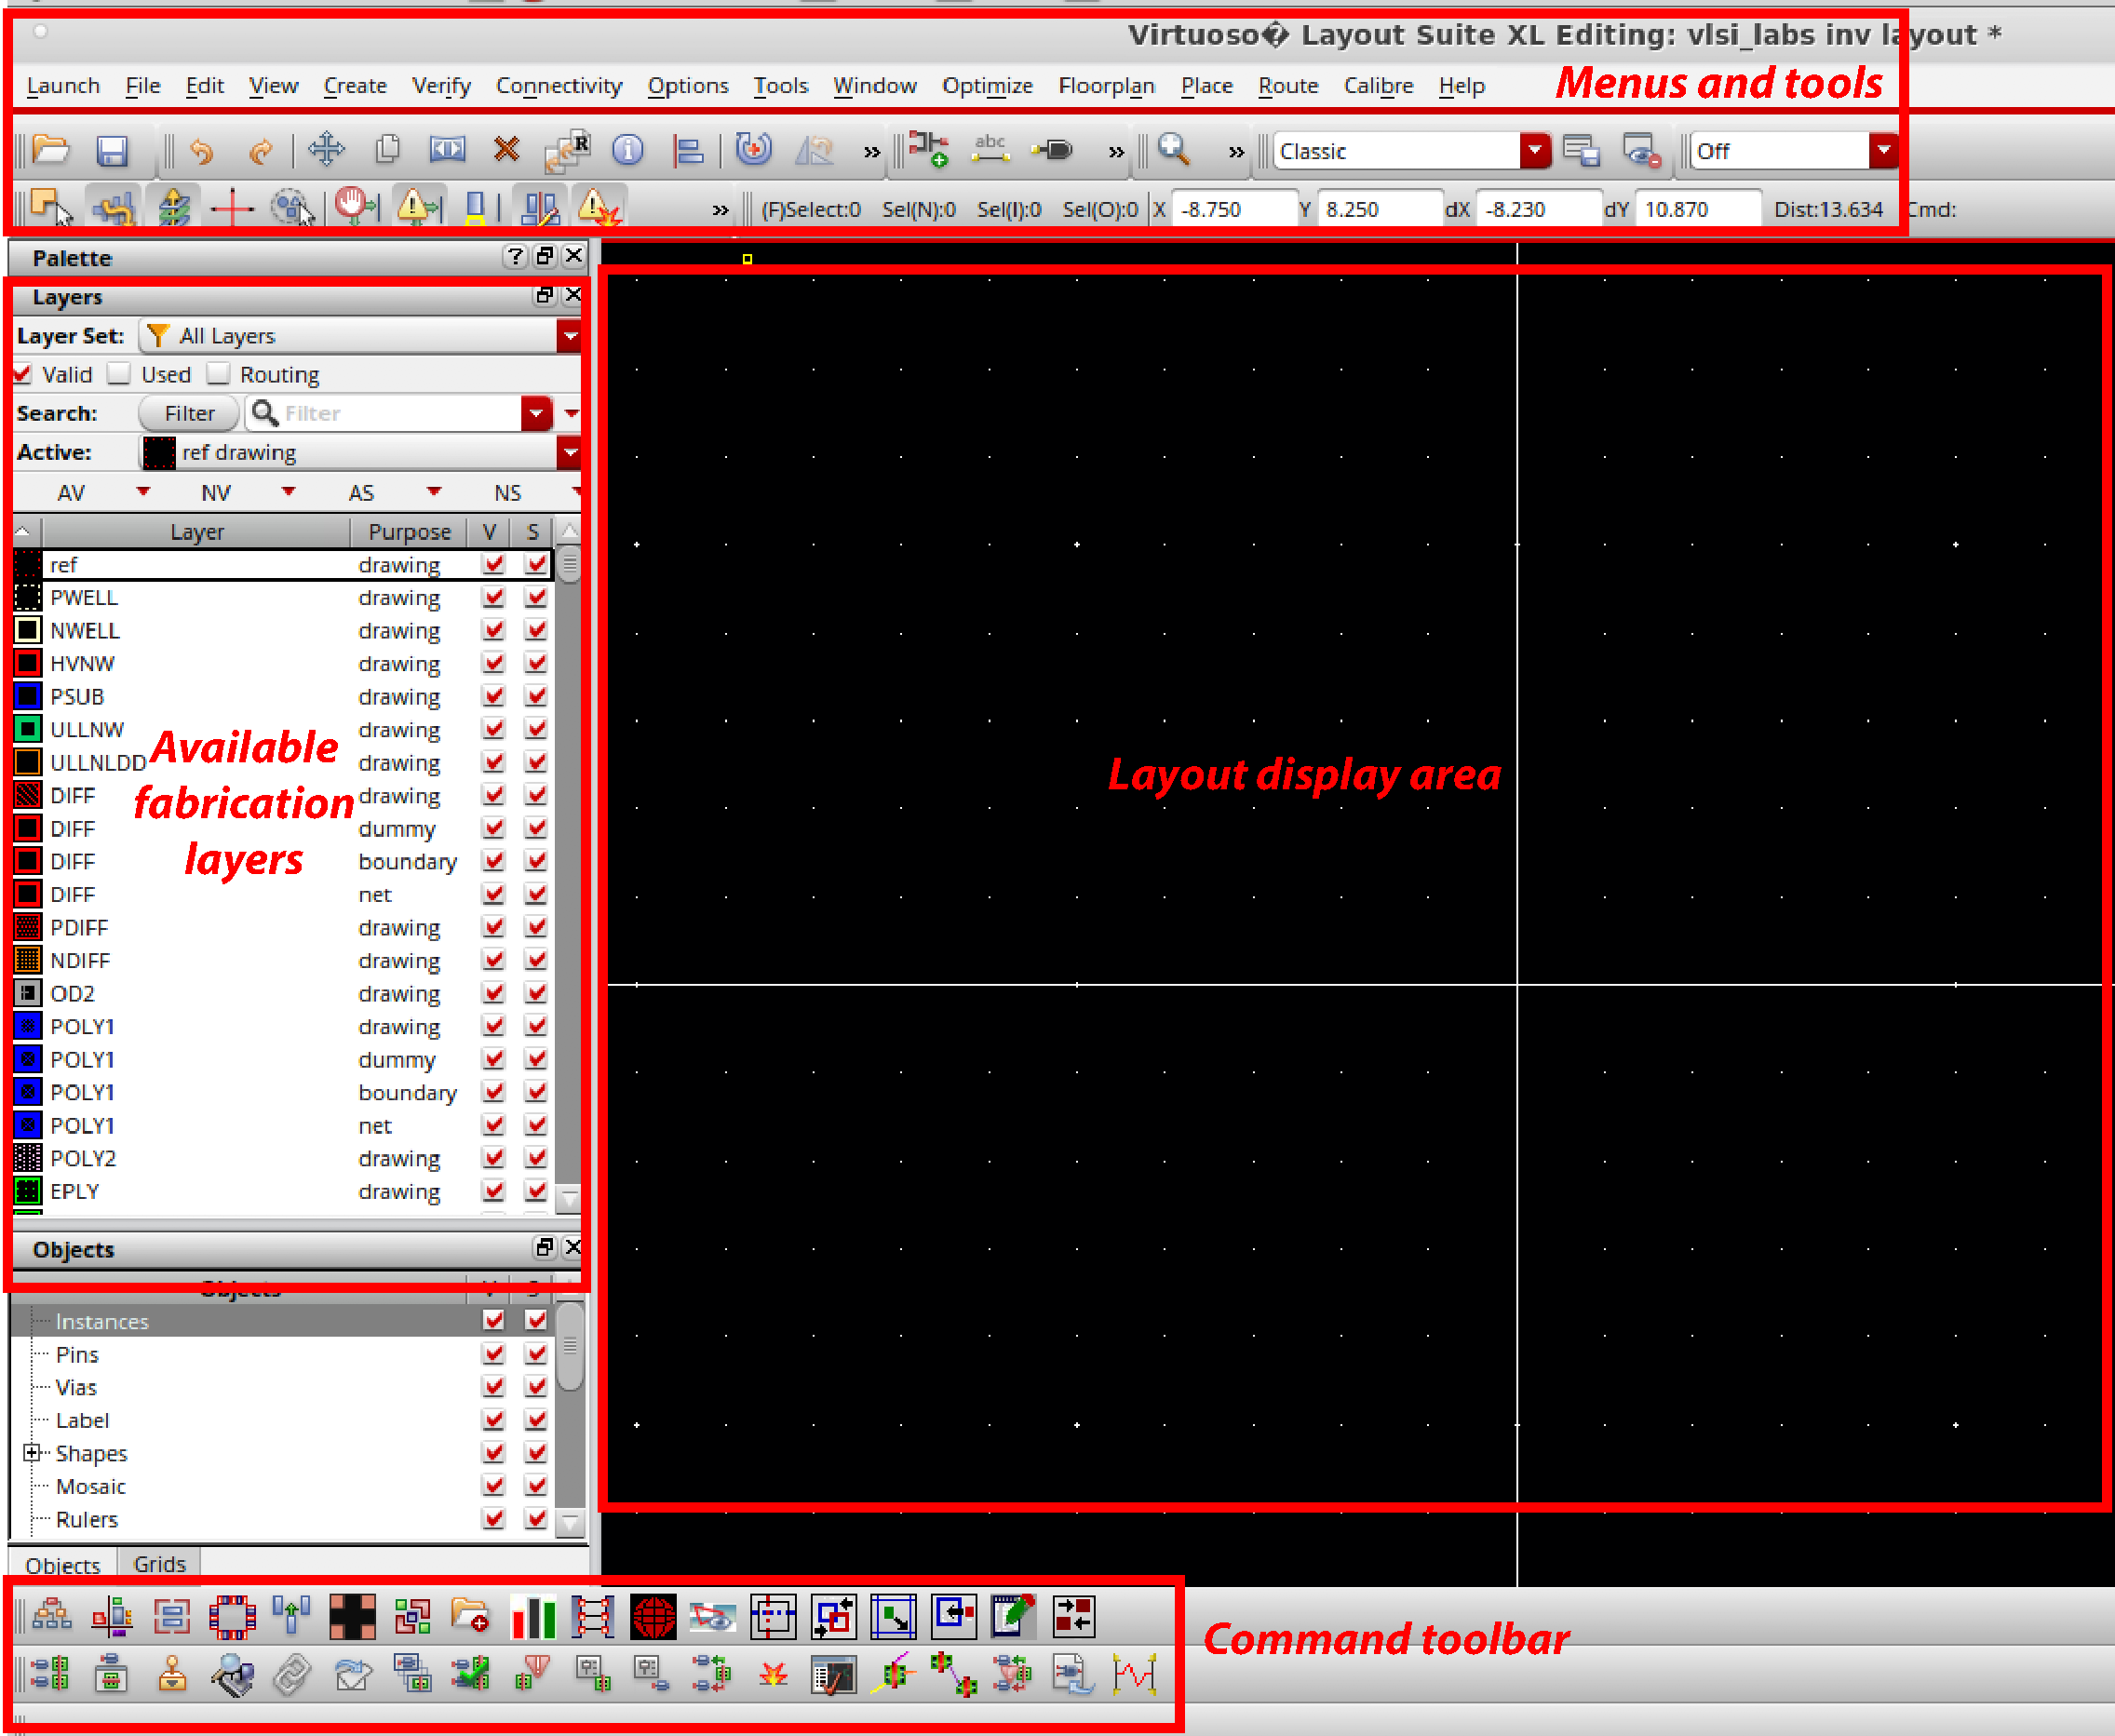
\includegraphics[scale=0.25]{figures/lab2_layout/layout.pdf}
			\caption{Layout XL window.}
			\label{fig_layoutwin}
		\end{wrapfigure}
		\item The Virtuoso\textsuperscript{\tiny\textregistered} Layout XL Editor window will appear. All available fabrication layers are listed in the layer sub-window on the left (Fig \ref{fig_layoutwin}). From here, you can select which current layers are visible (V) or selectable (S). You can also choose to only display the layers currently in use in your current layout but selecting \textit{Used}. Many useful commands can be found in the command toolbar below the layout display area. Most of the shortcuts to save, delete an instance, rotate a component, \textit{etc.} are located in the menus and tools area.
		As you saw in class, integrated circuits are manufactured through a lot of process steps and are composed by a large number of planar layers, stacked on top of each others. The layout is composed of the geometric shapes of each layers that corresponds to the actual pattern of those materials in your integrated circuit. Based on the layers you choose for your layout, precise masks will be generated during fabrication. This is why for a given layer (e.g. metal 1), several purpose layers are available (dummy, blockage, drawing).}
	\begin{remark}
		When closing your layout view and opening it again later, Layout L might be used instead. The only difference is that Layout XL contains more functionalities (such as instantiating the cells automatically, the ability to flatten your cells, \textit{etc.}). To switch, go to: \textit{Launch -> Layout XL}. 
	\end{remark}
	\clearpage
	As for the schematic view, lots of shortcuts are available in order to draw your layouts. The most important ones are given in Table. \ref{shortcuts}.

	\begin{table}[h!]
		\caption{Main Layout\textsuperscript{\tiny\textregistered} shortcuts.}
				\vspace{-2mm}
		\label{shortcuts}
		\centering
		\begin{tabular}{ |c| c|c| }
			\hline
			\textbf{Shortcut} & \textbf{Menu Access} &\textbf{Action}  \\ 
			\hline
			u & Edit -> Undo & Undo previous command \\  
			\hline
					c & Edit -> Copy & Copy selected instance(s)  \\  
			\hline
					m & Edit -> Move & Move selected instance(s)  \\  
			\hline
								s & Edit -> Stretch & Stretch selected layer  \\  
			\hline
			f & Window -> Fit All & Fit the entire design into the layout window  \\  
			\hline
			r & Create -> Rectangle & Create a rectangle shape  \\  
\hline
			i & Create -> Instance & Instantiate another design/layout in the current design  \\  
\hline
		o & Create -> Contact & Create a via/contact from the technology  \\  
\hline
		l & Create -> Label & Create a label for your pins  \\  
\hline
		q & Create -> Properties & Show the properties of selected instance  \\  
\hline
		k & Window -> Create ruler & Create a ruler to perform measurements  \\  
\hline
		ctrl+f & N/A & Shows the current level of hierarchy\\  
				& & All the instances in the lower levels are shown as red boxes  \\  
\hline
		shift+f & N/A & Shows all hierarchy levels. All the layers are shown  \\  
\hline
		\end{tabular}
	\end{table}
\end{enumerate}

\subsubsection*{Step 1: Transistors Instantiation}

	\begin{itemize}
\parbox[t]{\dimexpr\textwidth-\leftmargin}{%
	\begin{wrapfigure}[18]{r}{0.6\textwidth}
		\vspace{-6mm}
		\centering
		\vspace{-\baselineskip}
		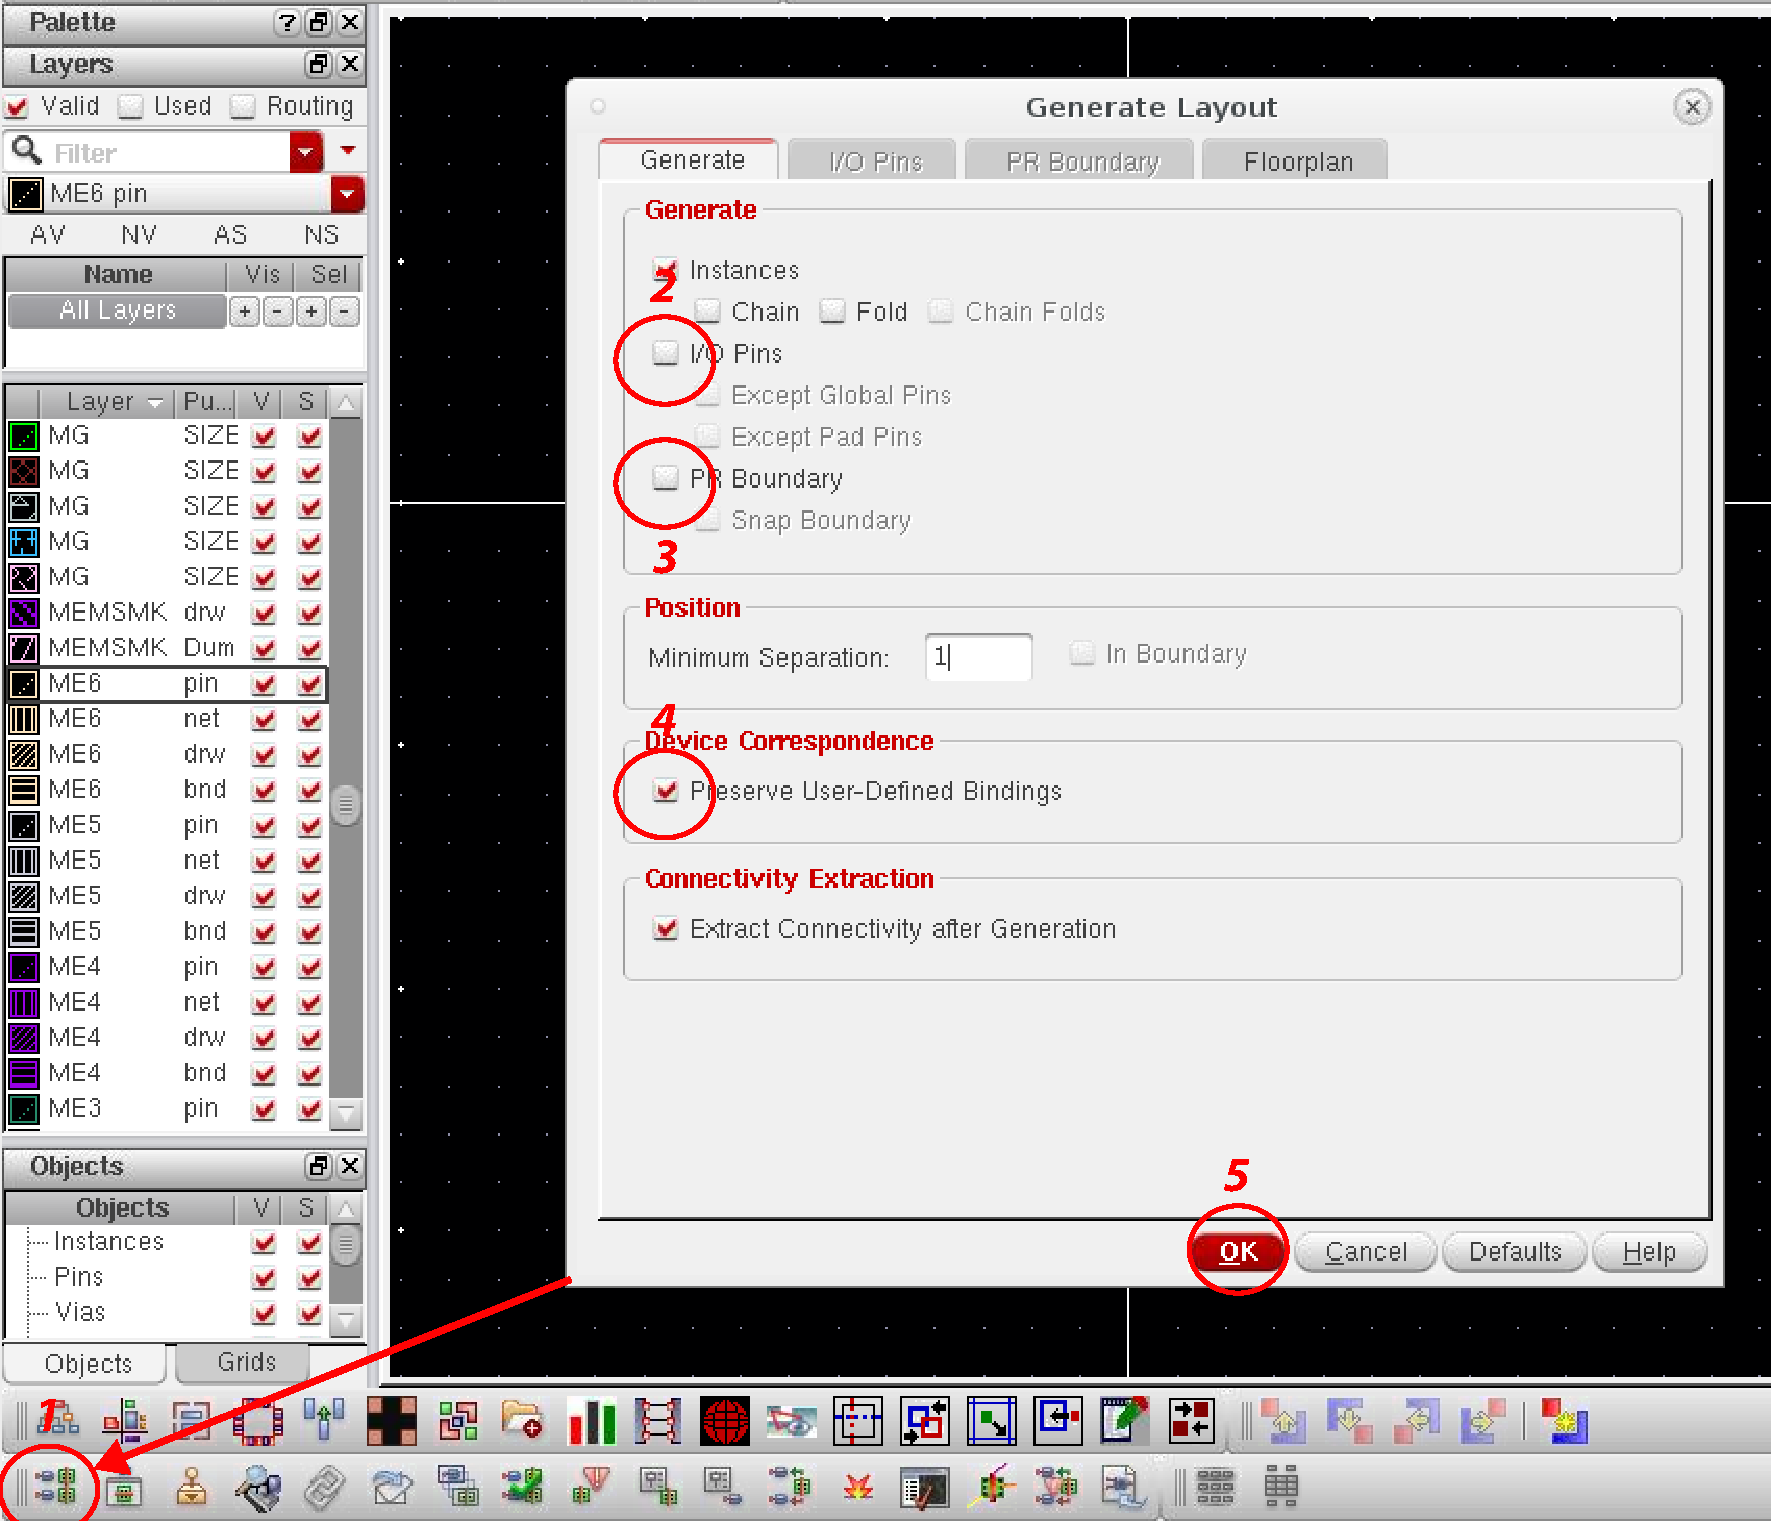
\includegraphics[scale=0.3]{figures/lab2_layout/layout_inst}
		\caption{Instantiating the transistors.}
		\label{layout_inst}
	\end{wrapfigure}
		\item Instantiate your transistors. To do so, from the layout editor Command Toolbar, choose Generate All From Source (as in Fig. \ref{layout_inst}), and set it up to generate only the instances and to preserve the device correspondence (mapping between the schematic and layout) and click OK.
		\item Your transistors should appear on the layout. \textbf{If all you can see is a red box with the transistors names, press \textbf{shift + f}}. It will allow you to display deeper levels of the hierarchy (here the several instances).}
	\end{itemize}


\begin{remark}
	Another way of instantiating your transistor is to press \textbf{i} and select the appropriate instance from one of the library, as you did for the schematic.
\end{remark}

\subsubsection*{Step 2: Placing your Transistors}
\parbox[t]{\dimexpr\textwidth-\leftmargin}{%
	\begin{wrapfigure}[24]{r}{0.32\textwidth}
		\vspace{-0mm}
		\centering
		\vspace{-\baselineskip}
		\includegraphics[scale=0.28]{figures/lab2/1}
				\caption{Using the ruler.}
	\end{wrapfigure}
	Now, let's place the $pmos$ transistor closer to the $nmos$. To do so, you need to move it vertically: press \textbf{m}, click on the $pmos$ transistor and move your mouse in the wanted direction. Here, we want the diffusion regions of our $nmos$ and $pmos$ to be distant by $.56 \mu m$. This distance is arbitrary for now, you don't have to necessary respect it for all your designs (the important distance to respect is the one between the power supply lines, which will bee explained in Step 6). To do so, we need to use some rulers:
	\begin{itemize}
		\item Press k to draw a ruler. To draw, select starting and ending points of the ruler by left-click after pressing k.
		\item You can always remove the existing rulers by pressing \textbf{Shift+k}.
		\item Use the ruler to check that the distance between both transistors is respected. If not, you need to move your transistors accordingly.
		\item Use the ruler again to make sure that the gate of both transistors are aligned. To do so, you can just place the ruler on the side of one of the gate and verify the alignment with the other gate.\end{itemize}
}


\subsubsection*{Step 3: Drawing the Poly-Silicon Gate Connection}
\parbox[t]{\dimexpr\textwidth-\leftmargin}{%
	\begin{wrapfigure}[28]{r}{0.5\textwidth}
		\vspace{-0mm}
		\centering
		\vspace{-\baselineskip}
		\includegraphics[scale=0.35]{figures/lab2/2}
		\caption{Poly-Silicon wire creation.}
		\label{layout_poly}
	\end{wrapfigure}
	Now, you need to connect the gate of the $nmos$ and $pmos$ together. To do so, you will draw a poly-silicon wire to connect both gates. 
	\begin{itemize}
		\item Select the poly-silicon layer on the drawing layers panel on the left by choosing $poly- drawing$, as depicted in Fig. \ref{layout_poly}.
		\item Press \textbf{p} and use the left mouse button to start and end the wire. For the starting point, select the top edge of the $nmos$ gate. For the ending point, select the bottom edge of the $pmos$. gate.\end{itemize}		\vspace{11mm}
}
	\begin{remark}
	It is possible to make the wire to break under a 90 degree angle if you use the left mouse button multiple times. However, at advanced technology nodes, it is generally harder to manufacture such kind of break lines due to the small size of the wires.
\end{remark}

\subsubsection*{Step 4: Placing the Poly-silicon to Metal1 Contact (Via)}
\begin{itemize}
	\item To draw the poly-silicon to metal 1 contact, multiple vias are necesary as there are multiple layers to traverse. Press \textbf{o} and select $PYL1_c$ as the Via Definition and then press $Hide$.
	\item Place your via on the poly-silicon wire as shown in Fig. \ref{layout_createvia}.
	\item This via will travel between the poly layer and the local interconnect layer. We must place one more via to get to the metal. Repeat the previous step with the $L1M1_c$ Definition and place it directly on top of the previous via.  \ref{layout_createvia}.
	\begin{figure}[!h]
		\centering
		\includegraphics[scale=0.32]{figures/lab2/3}
		\caption{Poly-silicon-Metal1 via creation.}
		\label{layout_createvia}
	\end{figure}
	
\end{itemize}


\subsubsection*{Step 5: Creating the Metal 1 Wire}
\parbox[t]{\dimexpr\textwidth-\leftmargin}{%
	\begin{wrapfigure}[28]{r}{0.5\textwidth}
		\vspace{-6mm}
		\centering
		\vspace{-\baselineskip}
		\includegraphics[scale=0.32]{figures/lab2/4}
		\caption{Local interconnect wire creation.}
		\label{layout_metal1}
	\end{wrapfigure}
	Now, you need to connect the drain of your $nmos$ and $pmos$ together to define your inverter output. To do so:
	\begin{itemize}
		\item Select the first level local interconnect layer on the drawing layers panel on the left by choosing $li1- drawing$. \ref{layout_metal1}.
		\item Press \textbf{p} and use the left mouse button to start and end the wire. For the starting point, select the top edge of the $nmos$ drain metal 1 area. For the ending point, select the top edge of the $pmos$ drain metal 1 area.\end{itemize}
}

\subsubsection*{Step 6: Creating the Metal 1 VDD and GND Supply Lines}


\parbox[t]{\dimexpr\textwidth-\leftmargin}{%
	\begin{wrapfigure}[28]{r}{0.13\textwidth}
		\vspace{-6mm}
		\centering
		\vspace{-\baselineskip}
			\includegraphics[scale=0.33]{figures/lab2/5}
\caption{Standard cell height requirements.}
\label{spacing}
	\end{wrapfigure}
	Now, you need to connect the drain of your $nmos$ and $pmos$ together to define your inverter output. To do so:
		\begin{itemize}
	\item Select MET1-drawing as a layer. Press \textbf{r} and draw a rectangle of random dimensions, as depicted in Fig. \ref{layout_rectangle}. Then select the metal 1 rectangle, click on \textbf{q} and change its width and height to $4.6 \mu m$ and $0.29 \mu m$ respectively.
			\begin{remark}
		You will learn later that integrated circuits are composed of many rows where each row contains standard cells (INV, MUX, \textit{etc}). \textcolor{red}{\textbf{Therefore, all of your standard cells need in this lab and the next ones need to have the same height}. For this technology, you need to ensure your supply line have an height of  $0.29 \mu m$. The standard cell height being $2.72kk \mu m$, you need to check that the spacing between both metal supply lines is $2.43 \mu m$, as depicted in Fig. \ref{spacing}.} In addition, the width of your cell needs to be a multiple of $4.6 \mu m$. Since the inverter is thinner than this, we chose to use $4.6 \mu m$.
	\end{remark}
	\item Place the metal 1 rectangle on top of the $pmos$ transistor, with a distance of $0 \mu m$ from the $NWELL$ layer as shown Fig. \ref{layout_rectangle}.
	\item Place a similar rectangle on the bottom of the $nmos$. To do so, press \textbf{c} (for copy), select the first metal 1 rectangle and move the second rectangle on the bottom, with a distance of $0.06 \mu m$ from the $nsdm$ (red) layer.. 
\end{itemize}
}

	\begin{figure}[!h]
		\centering
		\includegraphics[scale=0.33]{figures/lab2/6}
		\caption{Metal 1 rectangle creation and placement for the power supply lines.}
		\label{layout_rectangle}
	\end{figure}


\subsubsection*{Step 7: Finishing the Metal Connections}

\parbox[t]{\dimexpr\textwidth-\leftmargin}{%
	\begin{wrapfigure}[18]{r}{0.4\textwidth}
		\vspace{-6mm}
		\centering
		\vspace{-\baselineskip}
		\includegraphics[scale=0.25]{figures/lab2/7}
				\caption{Connecting the terminals to the supply metal lines.}
	\end{wrapfigure}
	Connect the source of the $nmos$ and $pmos$ to the appropriate power supply lines through the local interconnect layer. To do so:
	\begin{itemize}
		\item Press \textbf{p} and draw a line from the source of the $pmos$ to the $vdd$ power line. Double-click to confirm the line.
		\item Place a via that will connect the local interconnect and the metal 1 layers.
		\item Repeat the previous steps to connect the source of the $nmos$ to $gnd$.\end{itemize}
}


		\vspace{26mm}
\subsubsection*{Step 8: Creating the Bulk Taps}
\begin{itemize}
	\item Now, we need to create to connect the bulk of the $nmos$ and $pmos$ to $VDD$ and $GND$ respectively.
	\item Extend some local interconnect lines to the left from the vdd and ground pins on the pmos and nmos.
	\item At the end of each line, place a via that connects the tap and local interconnect layers (TPL1$\_$C).
	\item The VDD tap will need to be surrounded by a rectangle of the nsdm layer, and a rectangle of the nwell layer.
	\item The GND tap will need to be surrounded by a rectangle of the psdm layer.

	\begin{figure}[!h]
		\centering
		\includegraphics[scale=0.33]{figures/lab2/8}
						\caption{Creating the bulk taps.}
	\end{figure}
\end{itemize}

\subsubsection*{Step 9: Creating the Pins/Ports}

\parbox[t]{\dimexpr\textwidth-\leftmargin}{%
	\begin{wrapfigure}[20]{r}{0.6\textwidth}
		\vspace{-0mm}
		\centering
		\vspace{-\baselineskip}
		\includegraphics[scale=0.33]{figures/lab2/9}
		\caption{Creating Pins.}
		\label{pins}
	\end{wrapfigure}
	Now, we need to create the pins so the LVS tool will be able to compare the schematic and the layout connectivity.
	\begin{itemize}
		\item We need a pin for VDD, GND, A, and Z (Z will also need a via to metal first).
		\item To create a pin, go to Create -> Pin in the toolbar.
		\item Assure the name is the same as the net it will be place on, select rectange, and assure the io and signal types are correct. (In this example, "A" is an input signal.)
		\item Click $Hide$, and draw the pin rectangle over the targeted via (assure met1 - pin in the selected layer)
		\item Click on $Hide$ and place them on your layout.
		\item In this specific case with the "A" pin, there is only a metal via beneath the pin. You will need to place a metal 1 - drawing layer rectangle beneath the pin for it to be recognized. \ref{pins}\end{itemize}
}

\subsubsection*{Step 10: Labeling}

\parbox[t]{\dimexpr\textwidth-\leftmargin}{%
	\begin{wrapfigure}[20]{r}{0.6\textwidth}
		\vspace{-0mm}
		\centering
		\vspace{-\baselineskip}
		\includegraphics[scale=0.33]{figures/lab2/10}
		\caption{Final inverter layout.}
		\label{final_layout}
	\end{wrapfigure}
	Finally all the ports need to be labeled.
	\begin{itemize}
		\item Select the MET1-pin layer and go to: Create -> Label... (or press l).
		\item Write in a pin name (or all of them separated by spaces). They need to match the pins of your schematic.
		\item Set the label size to something resonable (~.3)
		\item Click on $Hide$ and place them on your layout
		\item Assure the name is the same as the net it will be place on, select rectange, and assure the io and signal types are correct. (In this example, "A" is an input signal.)
		\item Click $Hide$, and draw the pin rectangle over the targeted via (assure met1 - pin in the selected layer)
		\item Click on $Hide$ and place them on your layout.
		\item Your layout should be (mostly) complete now and look like Fig. \ref{final_layout}. In the next part, you will verify it and correct the potential errors.\end{itemize}
}

\clearpage
\subsection{CMOS Inverter Layout Verification}
In this part, you will learn how to perform all the necessary layout verification steps (DRC and LVS) and how to extract the parasitic values from your layout (PEX).
\subsubsection{DRC Verification}
Even if you followed the previous steps for the layout of your inverter, you will probable get some DRC errors. ($Hint$: 3 of these errors can be solved by extending the $diff$, $poly$, and $li1$ layers of the nfet downwards $.06 \mu m$)The goal of this part is for you to understand those errors and to correct those by yourself. To perform the DRC step:
	\begin{enumerate}

	\begin{figure}
		\vspace{-0mm}
		\centering
		\vspace{1cm}
		\includegraphics[scale=0.2]{figures/lab2_layout/drc_main}
		\caption{Calibre nmDRC main window.}
		\label{fig_drcmain}
	\end{figure}
	\parbox[t]{\dimexpr\textwidth-\leftmargin}{%
		\item Launch the Calibre DRC tool: from the layout view: \textit{Calibre -> Run nmDRC…}.
		\item The Calibre nmDRC window now appears (Fig. \ref{fig_drcmain}). Normally, you should not have to modify anything on the nmDRC window except for setting the runset file to:
		
		\begin{codeline}
			/uusoc/facility/cad$\_$common/skywater-src-nda/s8/V2.0.1/DRC/Calibre/s8$\_$drc$\_$runset
		\end{codeline}
		
		\item You can take a quick look at the different DRC settings to understand better how the tool work. For instance, if you click on \textit{Rules}, you can see what calibre rule file is selected to check your layout, as well as the different layers derivations.		\vspace{2mm}
}

\parbox[t]{\dimexpr\textwidth-\leftmargin}{%
	\begin{wrapfigure}[14]{r}{0.6\textwidth}
		\vspace{-0mm}
		\centering
		\vspace{-\baselineskip}
		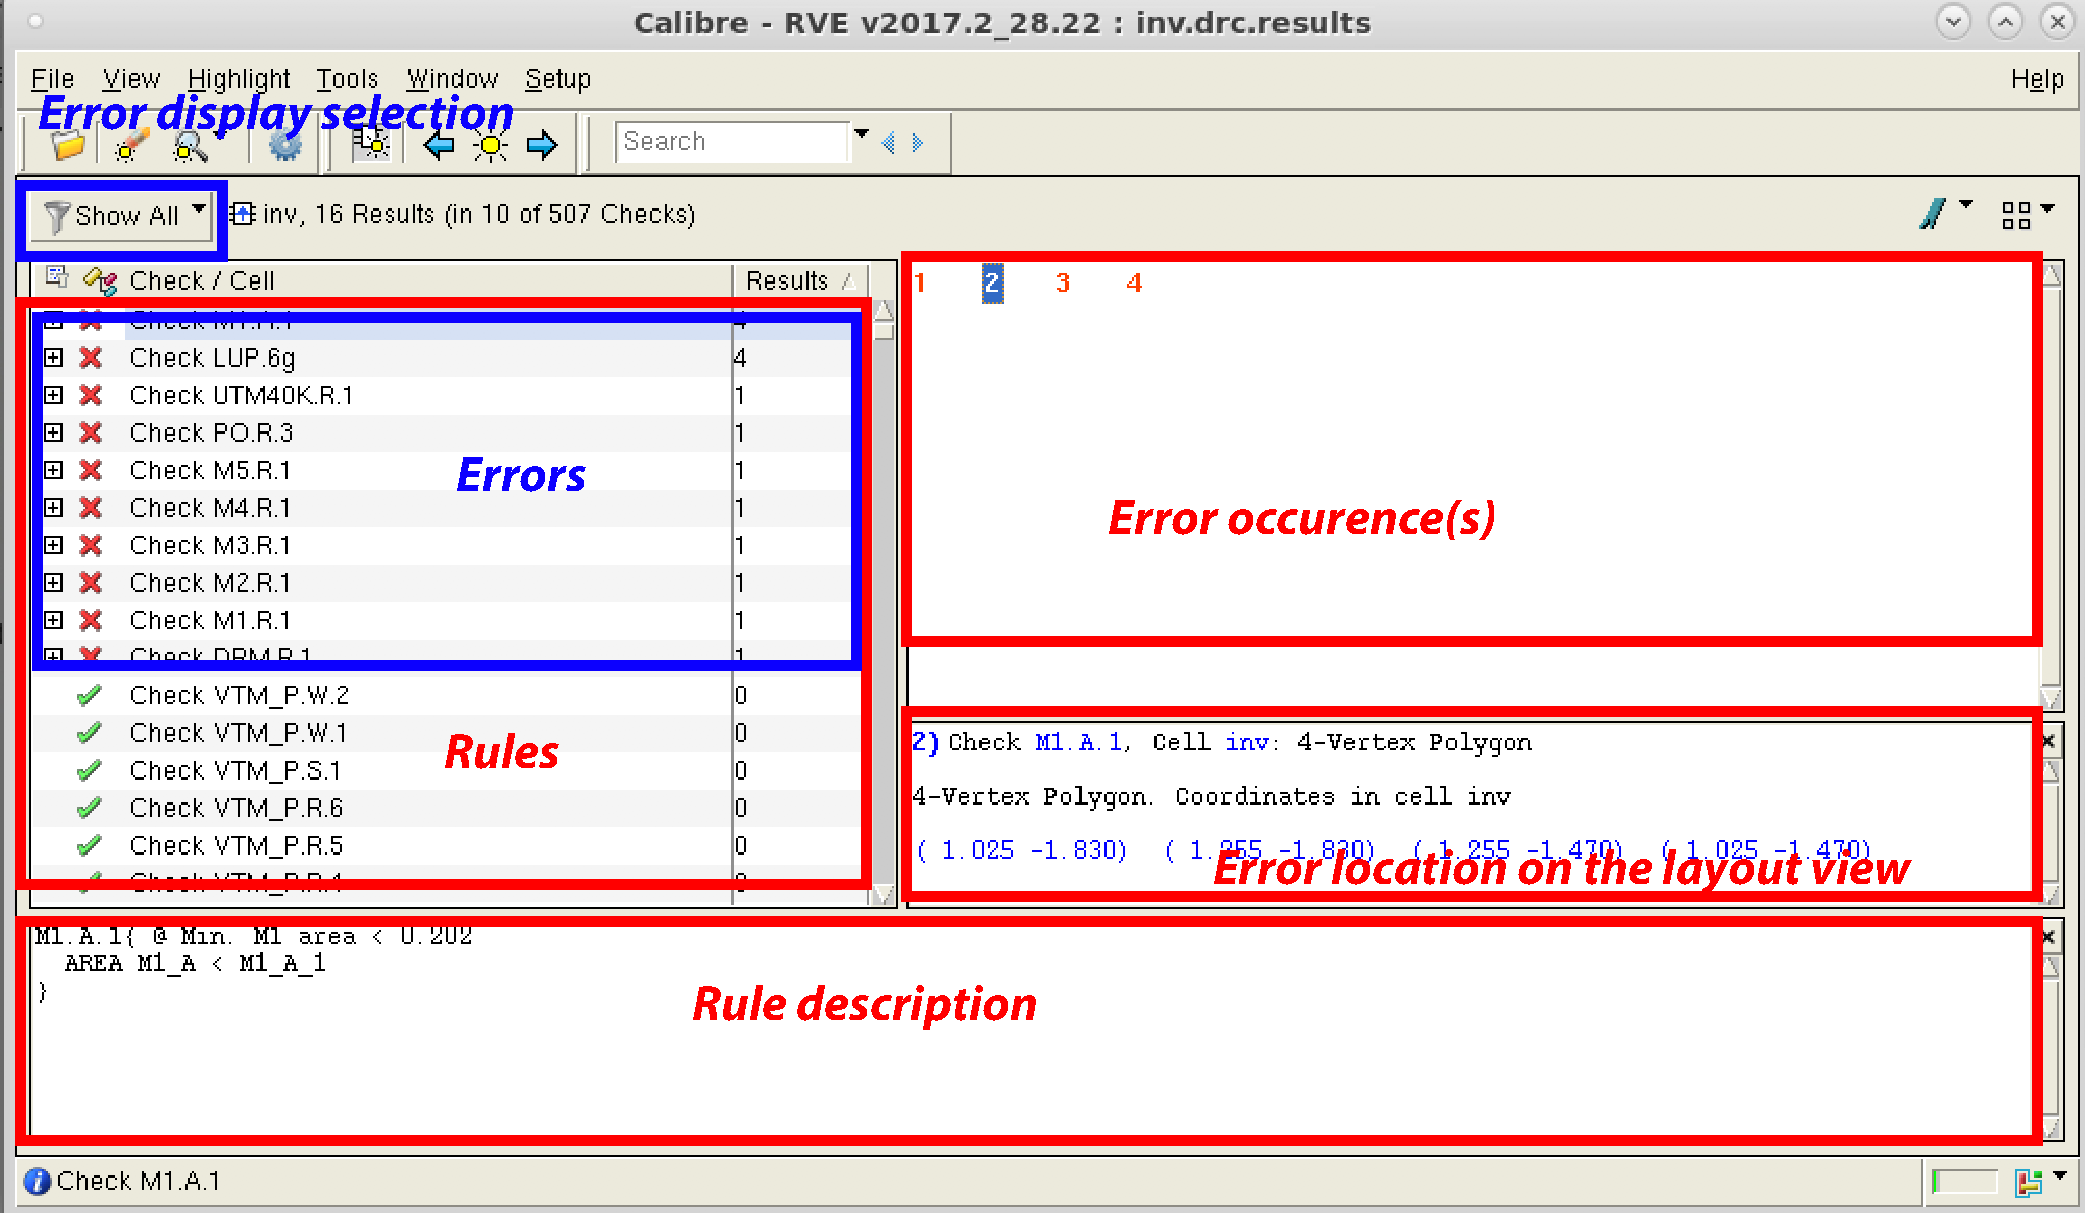
\includegraphics[scale=0.28]{figures/lab2_layout/drc_verif.pdf}
\caption{DRC result window}
\label{fig_drcverif}
	\end{wrapfigure}
	\item Then Click on Run DRC, wait a little bit and the potential DRC errors will be displayed. As shown in Fig. \ref{fig_drcverif}, a new window should appear. On the left pane are listed all the different rules. You can click on $Results$ to order them. If some rules have a red cross in front of them, it means your design does not respect some of the foundry rules (the goal is then to only have green symbol in front of every rules, otherwise, the foundry will not be able to manufacture your design). The rule description tells you what the rule require to be enforced. In this example, it says that the minimum metal 1 area should be at least $0.202 \mu m^2$. The error occurrence tells you how many occurrence of the same error you have in your design. The other pane tells you where the error is located. If you want to directly locate the error on your layout view, you can double click on the error number in the error occurrence pane (1 2 3 4 in Fig. \ref{fig_drcverif}). Once this error is corrected, you can go back to the DRC results window, select another error, locate it and so on and so forth.\vspace{2mm}
}

	\item Once you have corrected some errors, go back to the Calibre nmDRC window, click on Run DRC and check again how many error you get. You need to repeat this step until there is no DRC error at all in your design. You don't have to correct all the errors at once before running DRC again. 
	
	\begin{remark}
		It is often a good practice to correct some errors and run the tool again to see your progress (sometimes, by correcting some errors you might create new ones so it's better to go step by step). \newline
		When closing the DRC window, you will be asked if you want to save your changes to the runset file. Select \textit{No} and do the same when closing the LVS and PEX tools in the rest of the lab.
	\end{remark}
	
\end{enumerate}

\subsubsection{LVS Verification}

\begin{figure}
	\vspace{-0mm}
	\centering
	\vspace{1cm}
	\includegraphics[scale=0.25]{figures/lab2_layout/lvs_main}
	\caption{Calibre nmLVS main window.}
	\label{fig_lvsmain}
\end{figure}

\parbox[t]{\dimexpr\textwidth-\leftmargin}{%
	To perform the LVS step:
	\begin{enumerate}
		\item Launch the Calibre LVS tool: from the layout view: \textit{Calibre -> Run nmLVS…}.
		\item When the \textit{Load Runset File} window appears, browse and select: 
		\item The Calibre nmLVS window now appears (Fig. \ref{fig_lvsmain}). As for the DRC, you should not have to modify anything on the nmLVS window except setting the LVS runset file to:
		
		\begin{codeline}
			/uusoc/facility/cad$\_$common/skywater-src-nda/s8/V2.0.1/LVS/Calibre/s8$\_$lvs$\_$runset
		\end{codeline}

		\item Then Click on Run LVS, wait a little bit and the potential LVS errors will be displayed. A new LVS result window should appear. If your layout is correct, you should see the green smiley and icons as shown in Fig. \ref{fig_lvsverif}. If not, it means you have some errors. On the left pane are listed the different errors as follows:
\end{enumerate}}

%		\textit{$/research/ece/lnis-teaching$\newline$/5710\_6710/Runsets/$\newline$tsmc180nm\_lvs\_runset$} and click OK. The runset will define the settings of the LVS tools (in the same manner as before for the DRC). 

%\begin{figure}[!h]
%	\centering
%		\includegraphics[scale=0.4]{figures/drcrunset}
%\caption{LVS runset selection.}
%\label{fig_lvsrunset}
%\end{figure}
\begin{itemize}	
\parbox[t]{\dimexpr\textwidth-\leftmargin}{%
	\begin{wrapfigure}[24]{r}{0.62\textwidth}
		\vspace{0mm}
		\centering
		\vspace{-\baselineskip}
	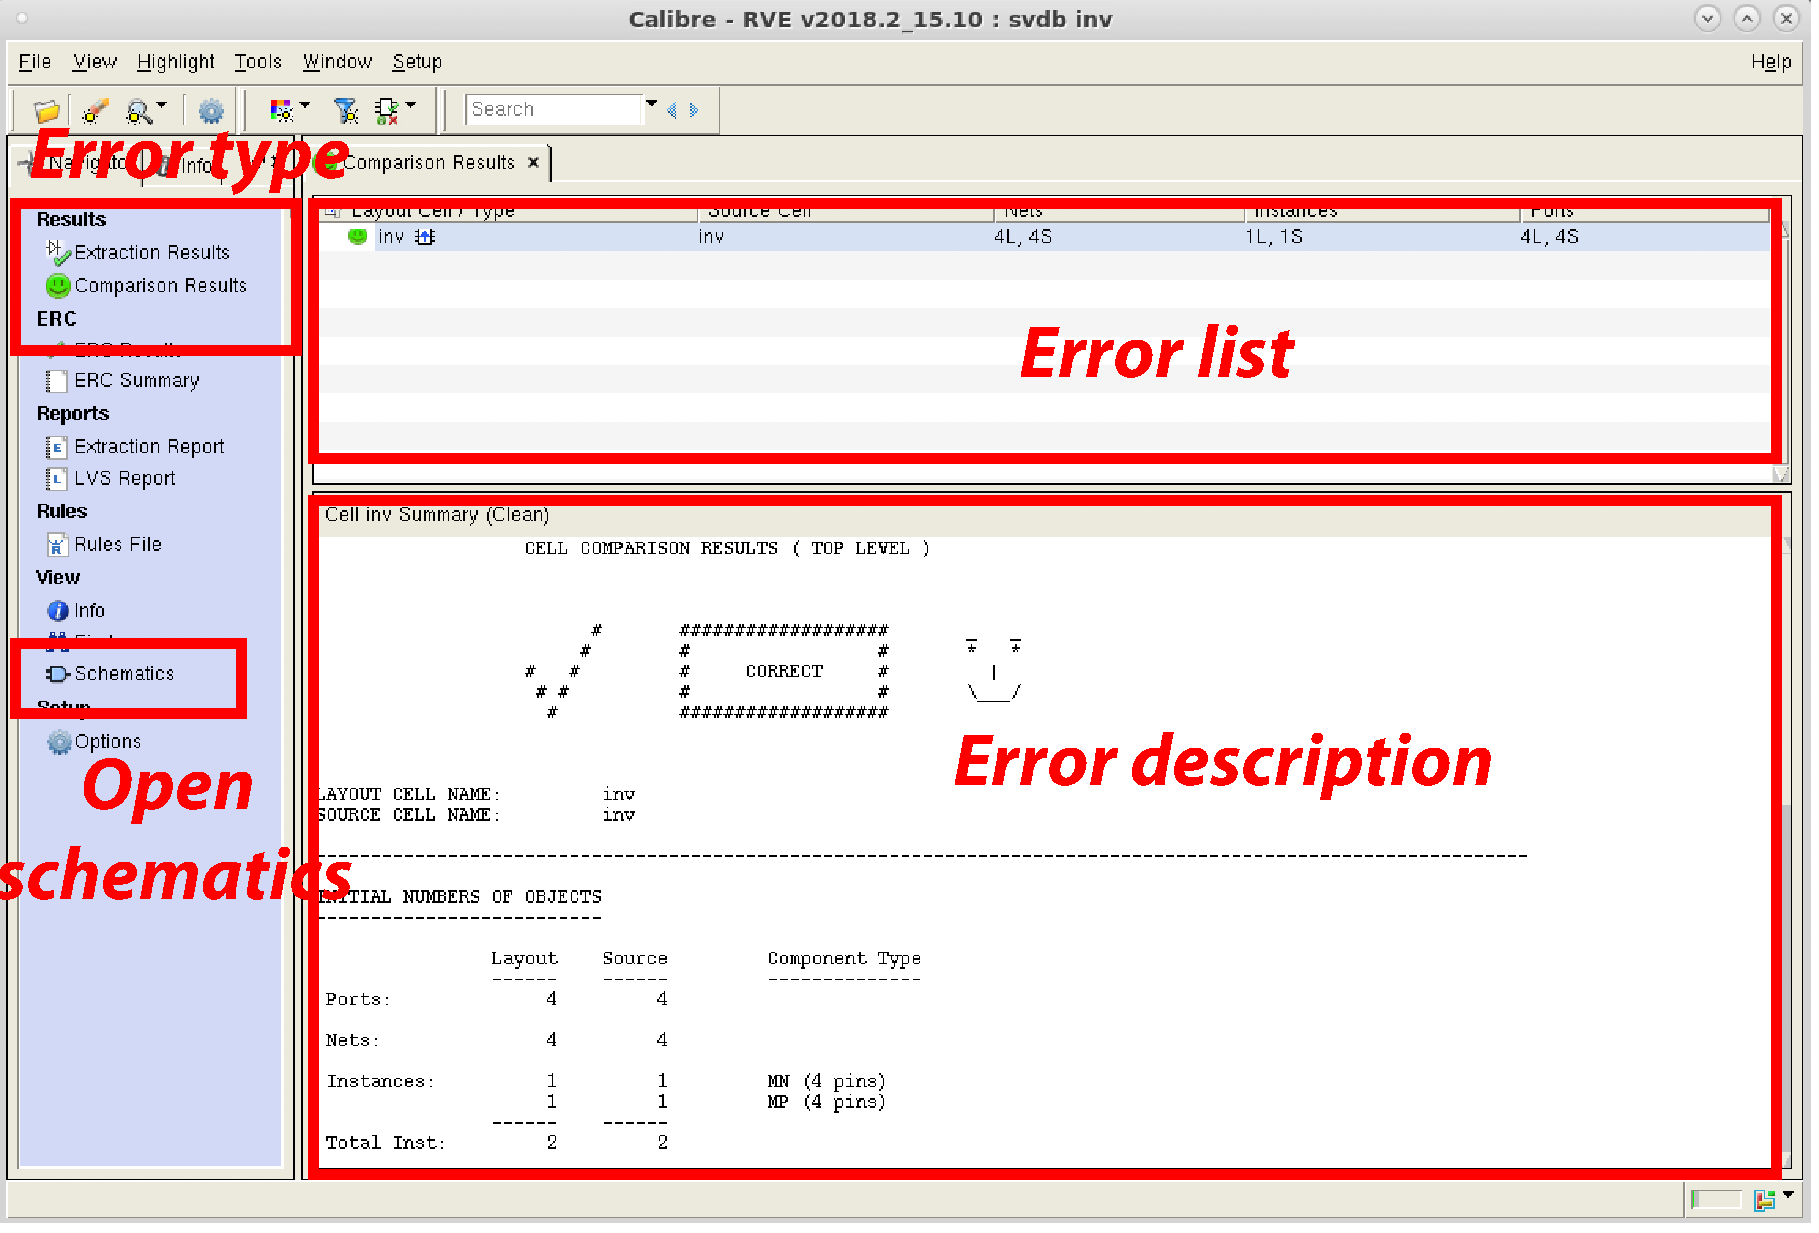
\includegraphics[scale=0.3]{figures/lab2_layout/lvs_verif}
\caption{LVS result window.}
\label{fig_lvsverif}
	\end{wrapfigure}
	\item \textbf{Extraction results} will list the pin related errors. For instance, if you define the same pin on two different nets, or if your design is missing the power supply or the ground pin, errors will be reported. 
	\item \textbf{Comparison results} will list the mismatches between your schematic and your layout. For instance, if you forget to connect the source of the \textit{nmos} of your inverter to the ground, an error will be reported.}
\end{itemize}


		\vspace{2mm}
To help you correct some LVS errors, Fig. \ref{fig_lvs_bad} shows an inverter design with some errors. In case you have some extraction errors, click on \textit{Extraction Results} and you will see the different errors in the error list. In Fig. \ref{fig_lvs_bad} (a), the error is caused by an absence of the power supply pin. To display the comparison errors, click on \textit{Comparison Results}. In Fig. \ref{fig_lvs_bad} (b), there are two errors: the nets $A$ and $Z$ can not be found in the layout since the pins have not been specified either. In some cases, an error could be caused by a bad connection (i.e. the input and output of the inverter could be connected together by a metal line). In the error description panel, you can click on the net names ($A$ and $Z$ in this case) and the associated net will be highlighted on either the source (schematic) or layout of your design. 

\begin{remark}
	Sometimes, it can be helpful to click on \textit{Schematics} on the LVS result window. It will open both the schematic of your design and the equivalent schematic of your layout. From here, you can visualize the difference and correct them. \newline
	As before, it is a good practice to correct some errors and run the tool again to see your progress.
\end{remark}

\begin{figure}[!h]
	\centering
	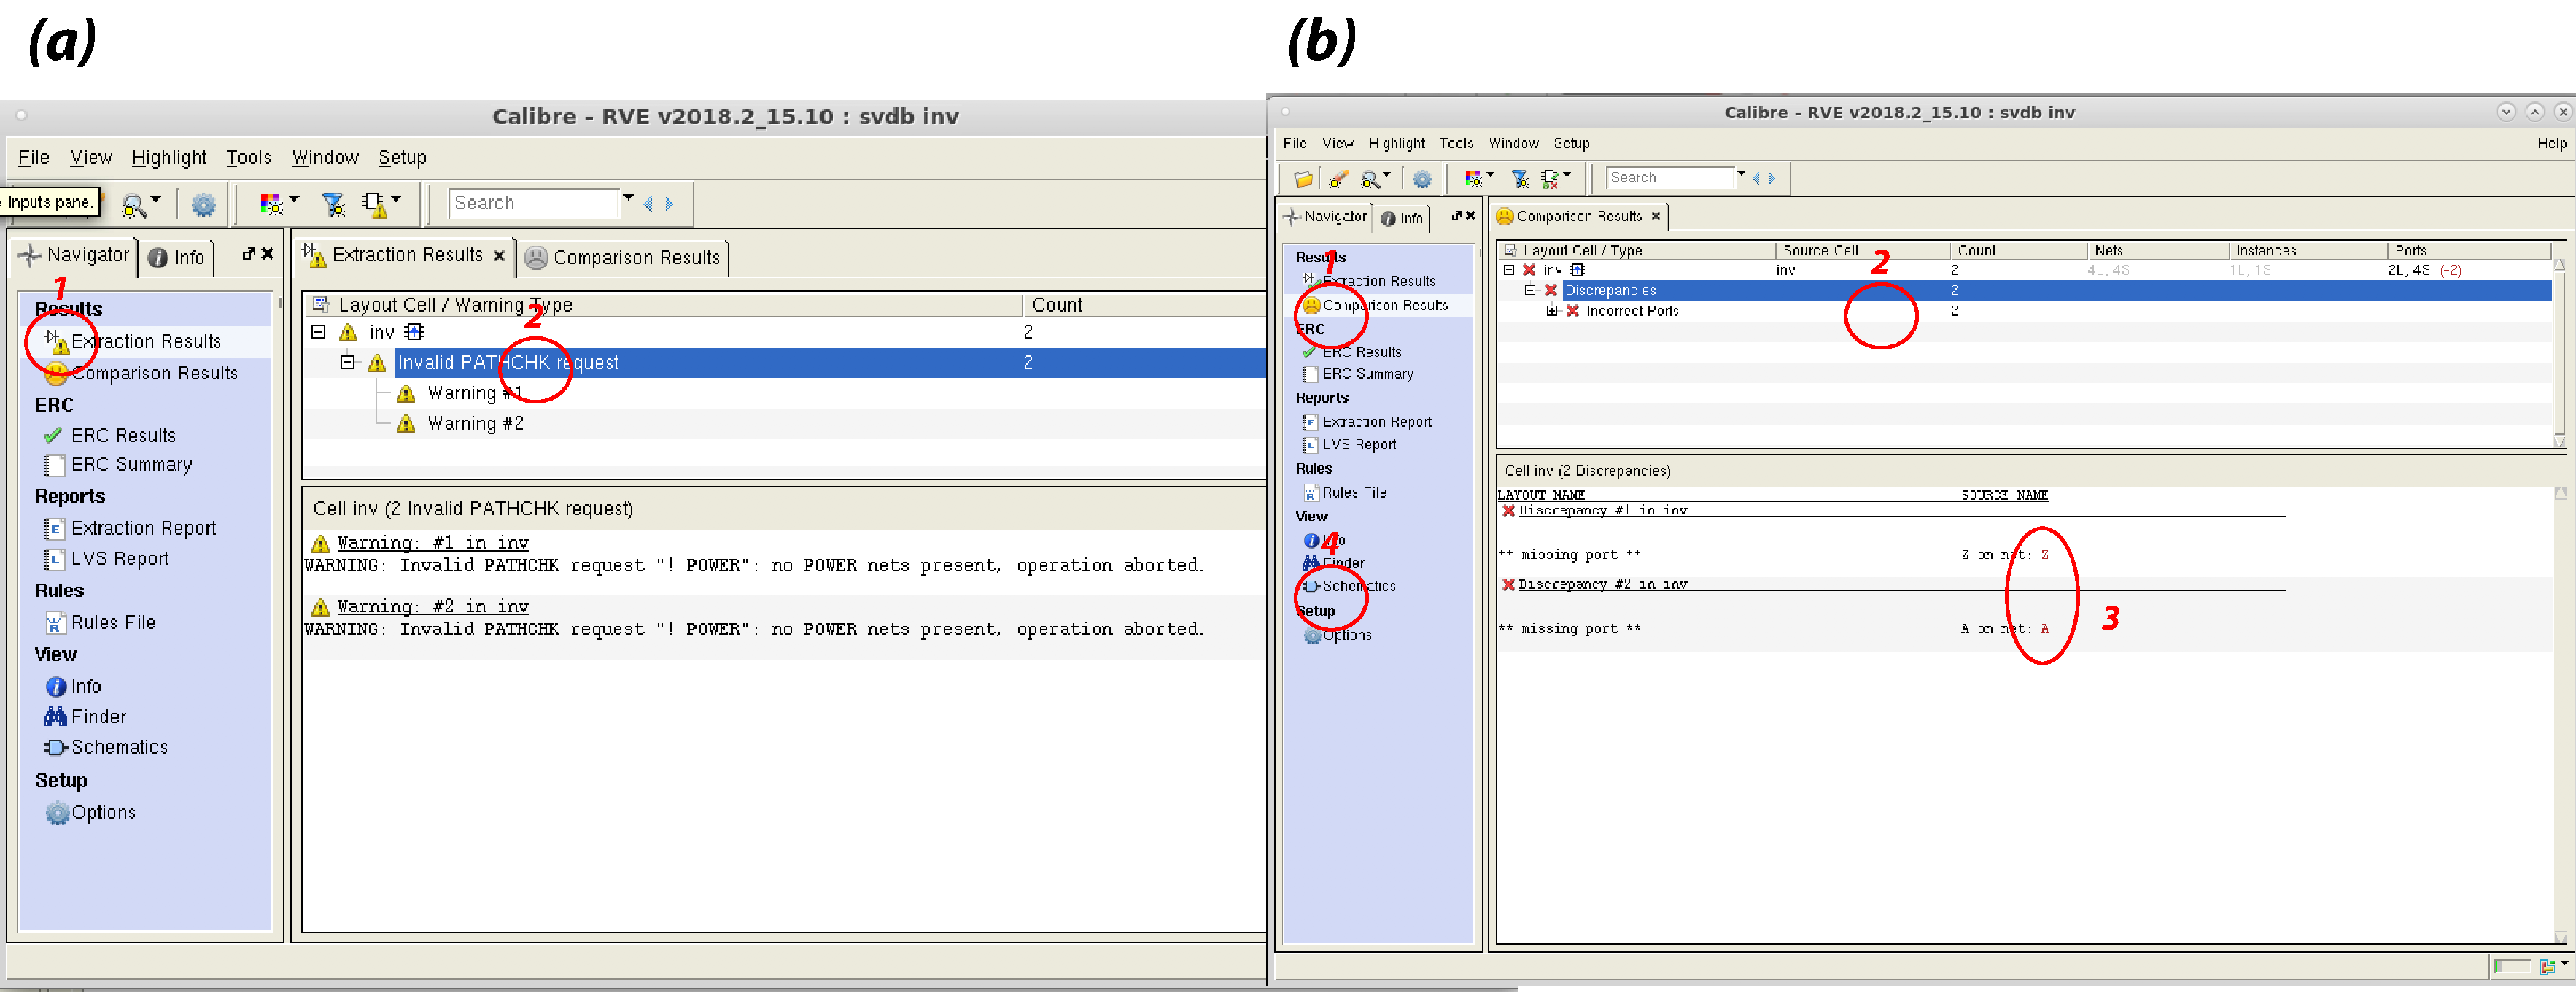
\includegraphics[scale=0.28]{figures/lab2_layout/bad_lvs}
	\caption{LVS result window for: (a) Extraction results; (b) Connectivity results.}
	\label{fig_lvs_bad}
\end{figure}

%\end{enumerate}

\begin{checkpoint}\label{check1}
	Please call an assistant and show him that your inverter design pass both the DRC and LVS with no errors.
\end{checkpoint}

\newpage 
\subsubsection{Parasitic Extraction (PEX)}
\begin{warning}
	The PEX step can only be done if your design is LVS compliant.
\end{warning}



\begin{figure}
	\vspace{-0mm}
	\centering
	\vspace{1cm}
	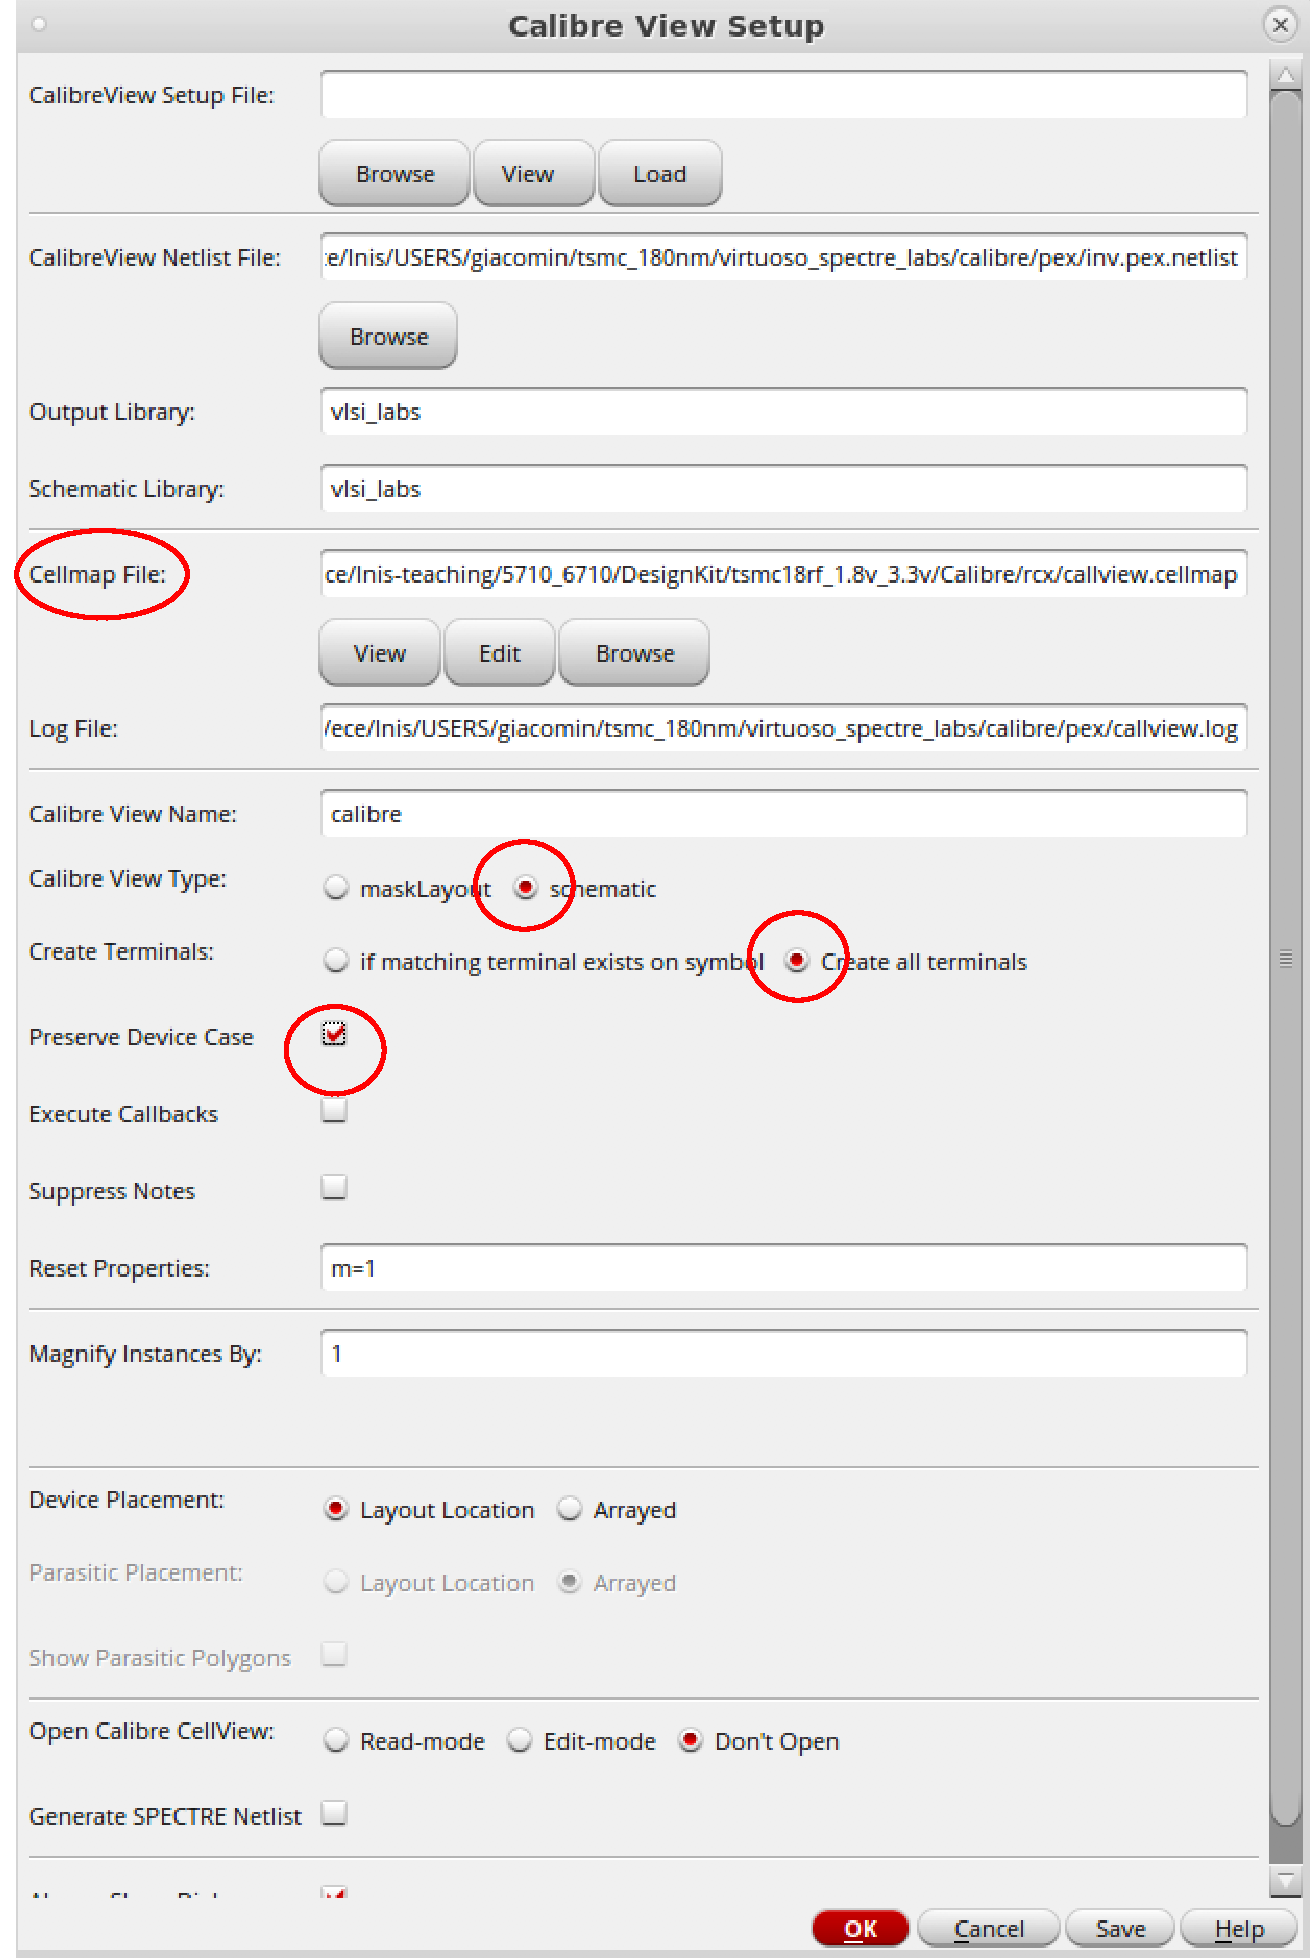
\includegraphics[scale=0.32]{figures/lab2_layout/pex_options.pdf}
	\caption{PEX options.}
	\label{fig_pex}
\end{figure}

\parbox[t]{\dimexpr\textwidth-\leftmargin}{%
	To perform the PEX step:
	\begin{enumerate}
		\item Launch the Calibre PEX tool: from the layout view: \textit{Calibre -> Run PEX…}.
		\item The Calibre PEX window now appears. Again, you normally should not have to modify any settings except setting the runset file to:
		
		\begin{codeline}
			/uusoc/facility/cad$\_$common/skywater-src-nda/s8/V2.0.1/PEX/xRC/Calibre$\_$PEX$\_$runset
		\end{codeline}

		\item Click on Run PEX.
		\item Then, a window will appear as depicted in Fig \ref{fig_pex}. Verify that the options (the important ones are highlighted in red) are the same as in Fig. \ref{fig_pex} (some fields, such as the library settings can of course differ depending on the name you chose).
		\item Click on $OK$ at the bottom of the window.
		\item You should get a pop-up window as shown in Fig. \ref{fig_pex_good} with no warnings.
		\item Once this is done, go back to the Library Manager window. You should be able to see a new view for your inverter cell in your working library named \textbf{calibre}. When you open it, you can see the resistances and capacitances modeling the parasitics of your layout.
		\begin{remark}
			Do not forget to check and save your calibre view (you might get some warnings but those are fine) before closing it. Otherwise, you will encounter an error when doing your post PEX simulation.
			\end{remark}
\end{enumerate}}

\begin{checkpoint}\label{check2}
	Please call an assistant and show him that the \textit{calibre} view for your inverter has been properly generated.
\end{checkpoint}


\begin{figure}[!h]
	\centering
	\includegraphics[scale=0.6]{figures/lab2_layout/pex_good}
	\caption{Successful PEX extraction.}
	\label{fig_pex_good}
\end{figure}

\subsection{CMOS Inverter Post Layout Simulation}
With technology scaling, the RC delay is now a big issue due to the increased parasitics. This is why it is important to perform a post layout simulation which takes into account the parasitics (after the PEX step). 
\begin{enumerate}
	\item Go to the library manager and open the schematic view of your inverter transient testbench ($inv\_testbench\_tran$).
	\item Launch ADE L. From the ADE window, open up the state you previously defined in the previous part: click on \textit{Session -> Load State ...}. A new window will appear, simply click on \textit{Ok}.
	\item Now, all the settings you previously defined (parameters values, analysis type, display output) should be there.
	\item To take into account the parasitics of your layout, we need to tell ADE to consider the parasitics in the simulation. To do so, go to the ADE window and go to: \textit{Setup -> Environment} and add the \textbf{calibre} view in first in the \textit{Switch View List}, as shown in Fig \ref{fig_simpex}.
	\item Click OK and launch the simulation. 
	\item Observe the output curves to check that your inverter behaves properly as well as how the delay changed compared the the simulation you ran before considering the parasitics.
	\begin{figure}[!h]
		\centering
		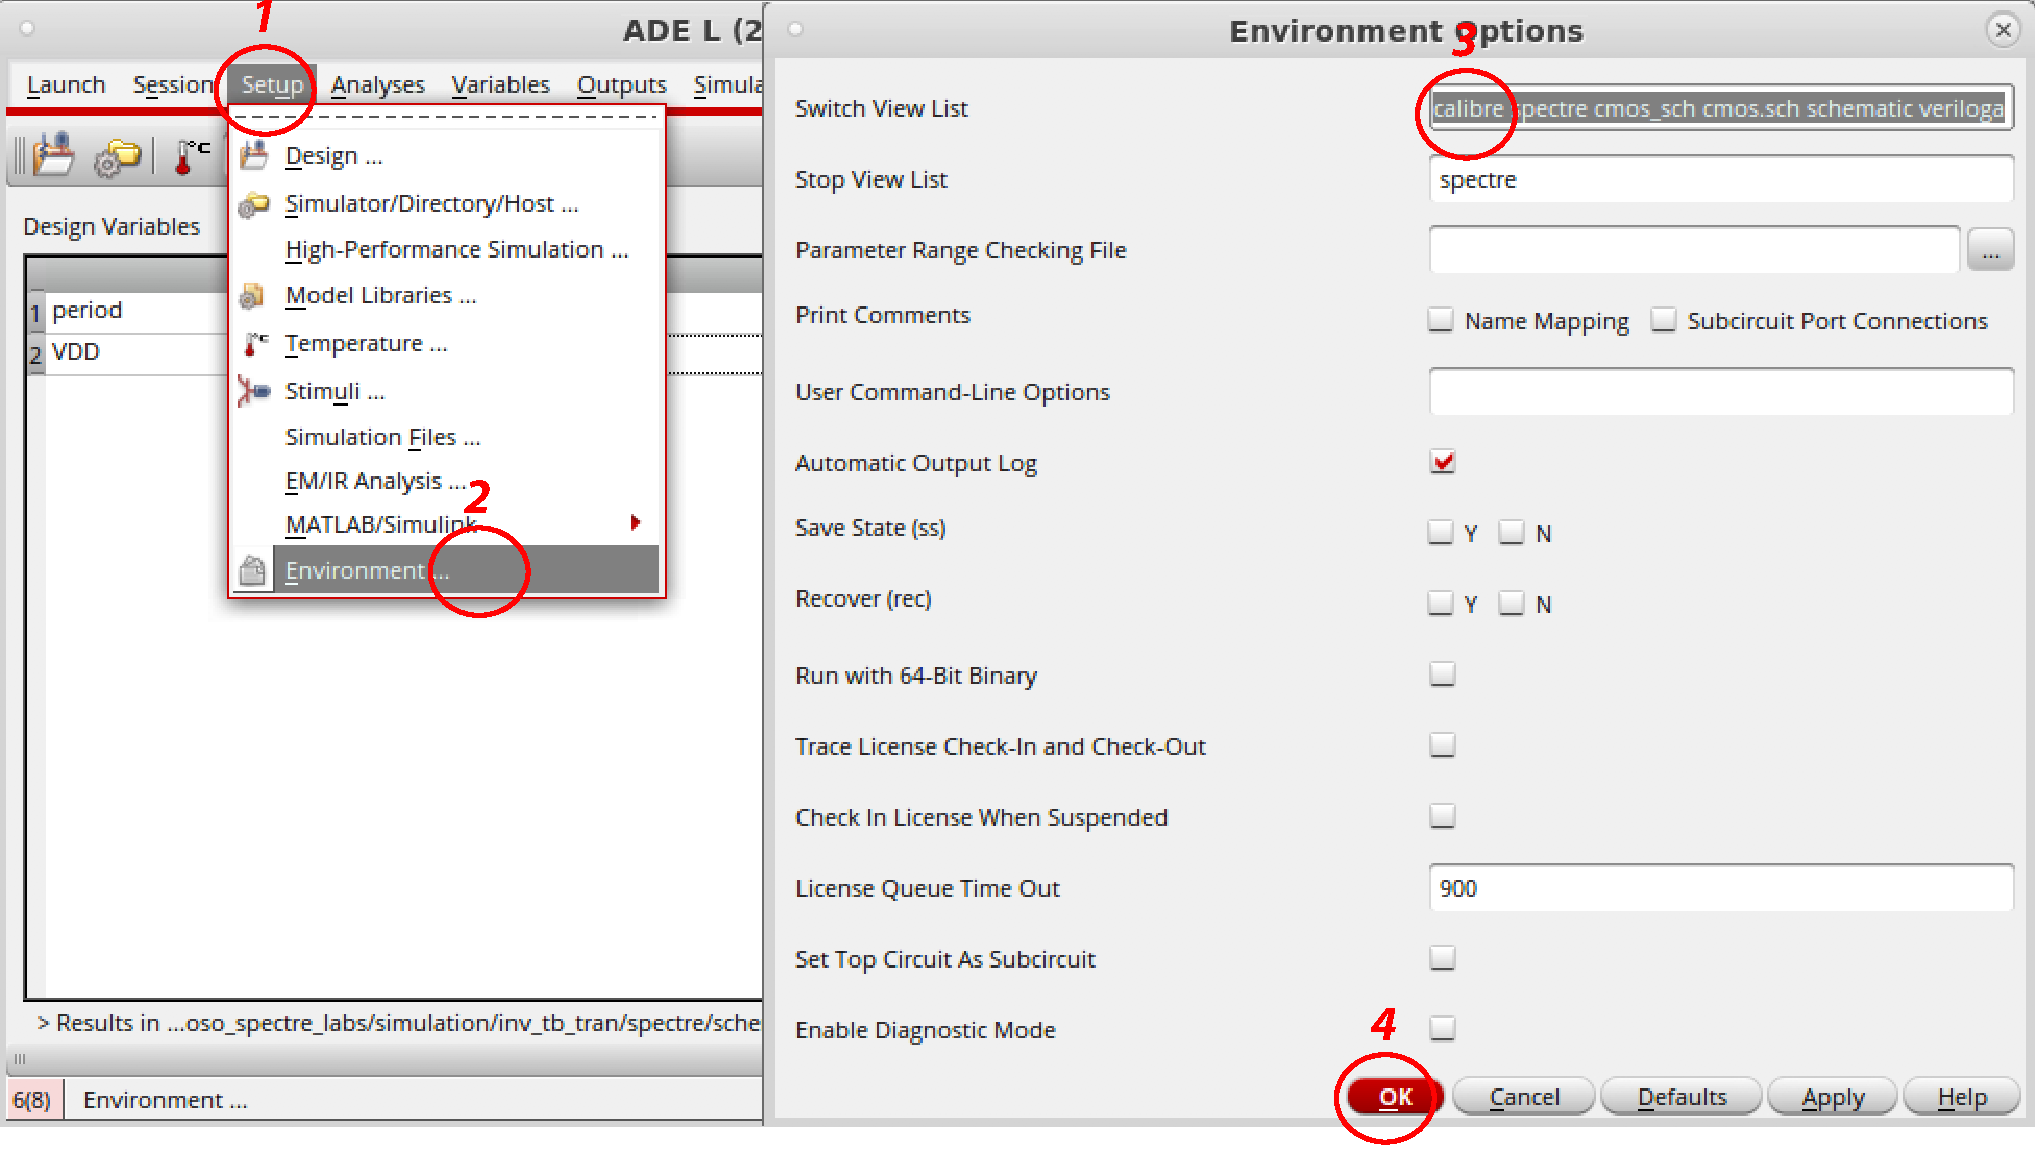
\includegraphics[scale=0.45]{figures/lab2_layout/ade_pex}
		\caption{ADE L environment options.}
		\label{fig_simpex}
	\end{figure}
	
	%\begin{remark}
	%	If you open the calibre view, you won't be able to save it because of a bug and you will not be able to run the simulation since you will get an error message saying that the calibre view is not saved. To be able to run the simulation by considering the calibre view, you will need to run the PEX again without opening the calibre view and then run your simulation.
	%\end{remark}
\end{enumerate}

	\begin{exercise}\ 
Report the rising, falling and propagation delays of your inverter after the PEX step. How did the delay change when compared to the pre-layout simulation? Why?		
\end{exercise}
\clearpage


\section{Assignment and Checkpoint Summary}
Write a report and answer the assignments asked during the lab, which are summarized below. Do not forget to validate the checkpoints, summarized below as well, by an assistant before the end of the lab.


	\begin{exercisesum}\	
			\vspace{-2mm}
	\begin{enumerate}
\item Report the rising, falling and propagation delays of your inverter after the PEX step. How did the delay changed when compared to the pre-layout simulation? Why?		
\item Provide a screenshot of the DRC result window as well as the LVS result window for the inverter, showing the correctness of your design.			
	\end{enumerate}
\vspace{-5mm}
\end{exercisesum}	

\begin{checkpointsum}\
	\vspace{-2mm}
		\begin{enumerate}
	\item Please call an assistant and show him that your inverter design pass both the DRC and LVS with no errors.
	\item Please call an assistant and show him that the \textit{calibre} view for your inverter has been properly generated.
		\end{enumerate}
	\vspace{-5mm}
\end{checkpointsum}





\newcommand{\labtitle}{ECE/CS 5710/6710 - Lab 3}
\newcommand{\labsubtitle}{Synthesis of a MIPS Processor}
\vlsiheader

\begin{center}
\LARGE\textbf{\labsubtitle} \\
	\large\textbf{Pre-lab Assignment:} Check for the date on Canvas. \\
	\large\textbf{Lab Report:} Check for the date on Canvas.
\end{center}
\section{Objective}
This lab presents the main steps for performing the RTL/logic synthesis of an 8-bit MIPS microprocessor from the \textit{CMOS VLSI Design} book, using the Skywater 130 \emph{nm} design kit. This lab details the typical steps of the logic synthesis in VLSI design. The tool you will use is Synopsys Design Compiler\textsuperscript{\tiny\textregistered}, which is widely used in industry and academia. 



\section{Pre-lab Assignment}
\begin{prelab}
	Answer the following questions and submit a \textbf{.pdf} file through Canvas:
 \begin{enumerate}
 	\item What RTL stands for? Explain briefly the different levels of abstraction in VLSI design.
 	\item Explain briefly what is logic synthesis in VLSI design.
 	\item What is a timing library and what does it contain? Why do you need it for the synthesis flow?
 \end{enumerate}
\vspace{-5mm}
\end{prelab}


\section{Directory Organization}

For the logic synthesis, it will be simplest to work from a \textit{design$\_$compiler} folder. This folder has been added to the git repo. If it does not exist, the repo can be updated with:

\begin{codeline}
	git pull
\end{codeline}

This folder contains different subdirectories as follows:
 \begin{itemize}
\item \textit{DDC}: design database, where you will save your design after the different steps of the synthesis.
\item \textit{RPT}: report files (area, gate etc.) created by the tool.
\item \textit{SDC}: system design constraint file created by the tool.
\item \textit{SCRIPTS}: contains a TCL script to automatize the synthesis step (to be used at the end of the lab).
\item \textit{SDF}: Timing files created by the tool for functional verification.
\end{itemize}





\section{Lab Assignment}


\subsection{Starting Synopsys Design Compiler\textsuperscript{\tiny\textregistered}}
Launch the Synopsys Design Compiler\textsuperscript{\tiny\textregistered} GUI by going in your \textit{design$\_$compiler} folder and doing:
	\begin{codeline}
	design$\_$vision
\end{codeline}

The \textit{design$\_$compiler} directory contains an hidden file named \textit{.synopsys$\_$dc.setup}. This file is read every time Synopsys DC starts.
It specify what is the target library (the library that defines the area/timing/power characteristics of the physical logic gates) so in our case the standard cells from Skywater 130 \emph{nm}).\\


When Synopsys DC is opened, you will obtain a window as shown in Fig \ref{fig_syn_dc}. The \textbf{\textcolor{blue}{Console terminal}} is used for entering Design Compiler (DC) commands, to source Tcl scripts or to run Linux commands. Those things can also be done through the \textbf{\textcolor{blue}{command line}} through a script. The lab will show you how to perform the tasks with the GUI by hand, but it can be automatized by running command lines. In addition, not all commands are available in the GUI. For more complex and repetitive synthesis tasks, it is highly recommended to use scripts. When you will perform actions on the GUI, the equivalent commands will be recorded and stored in the \textit{command.log} file in the \textit{design$\_$compiler} directory. The equivalent commands will also be given in this tutorial. To obtain some help about a command, you can run in the console terminal or the command line: 	

	\begin{codeline}
	man your$\_$command
\end{codeline}


\begin{figure}[!h]
	\centering
	\includegraphics[scale=0.33]{figures/lab3_design_compiler/synopsys_overall.pdf}
	\caption{Synopsys DC window organization}
	\label{fig_syn_dc}
\end{figure}



The console terminal and the \textit{Log} view contain the trace of the execution of the command. The \textit{History} tab contains the history of all executed commands in the session.

\subsection{Analyzing the Verilog RTL Files}

	\parbox[t]{\dimexpr\textwidth-\leftmargin}{%
	\begin{wrapfigure}[11]{r}{0.4\textwidth}
		\vspace{-6mm}
		\centering
		\vspace{-\baselineskip}
 		\includegraphics[scale=0.5]{figures/lab3_design_compiler/analyze_dc}
\caption{Analyzing the Design}
\label{fig_analyze_dc}
	\end{wrapfigure}
	The analysis phase will compile the Verilog or VHDL source files and ensure that they are synthesizable (that means that they only contains statement that have meaning for synthesis, i.e. that can be mapped into a hardware circuit). To analyze the files, do:
	 \begin{enumerate}
		\item \textit {File -> Analyze...}
		\item Click on the \textit{Add...} button, as shown in Fig \ref{fig_analyze_dc} to select the Verilog file of the 8-bit microprocessor (\textit{mips.sv}). It is located in the \textit{HDL/RTL} folder.
		\item Click on OK.	
	\end{enumerate}
}

Equivalent DC command:
	\begin{codeline}
	analyze -library WORK -format sverilog $\{$.../HDL/RTL/mips.v$\}$
\end{codeline}

\subsection{Elaborating the Design}

	\parbox[t]{\dimexpr\textwidth-\leftmargin}{%
	\begin{wrapfigure}[11]{r}{0.4\textwidth}
		\vspace{-6mm}
		\centering
		\vspace{-\baselineskip}
		\includegraphics[scale=0.45]{figures/lab3_design_compiler/elaborate_dc}
\caption{Elaborating the design}
\label{fig_elaborate_dc}
	\end{wrapfigure}
This phase will perform a pre-synthesis of the netlist. It will basically identify the logic functions and the different registers (latches and flip-flops) that will be inferred. To elaborate the design, do:

\begin{enumerate}
	\item \textit {File -> Elaborate...}
	\item Select the top module of the verilog netlist: \textit{Processor}, as shown in Fig \ref{fig_analyze_dc}. 
	\item Click on OK.	
\end{enumerate}
}




Equivalent DC command:
	\begin{codeline}
elaborate mips -architecture verilog -library DEFAULT
\end{codeline}


On the \textbf{\textcolor{blue}{Log window}}, you can see the inferred registers for the different modules, as shown in Fig \ref{fig_registers}, their size (width) and their Set/Reset signals (AR/AS: asynchronous reset/set, SR/SS: synchronous reset/set). 

	\begin{figure}[!h]
	\centering
	\includegraphics[scale=0.5]{figures/lab3_design_compiler/registers}
	\caption{Some of the inferred registers}
	\label{fig_registers}
\end{figure}

On the \textbf{\textcolor{blue}{Hierarchy view}}, you can now see the inferred components and the associated standard logic cells. Select the \textit{andblock} from the \textit{alunit} module, as shown in Fig. \ref{fig_cellall} and select \textit{Cells (All)} at the top of the design view. It is also possible to display the elaborated schematics. Lets do it for the \textit{andblock}. To do so, make sure that the \textit{andblock} instance is selected in the hierarchy view and click on the \textit{Create Design Schematic} icon, as depicted in Fig. \ref{fig_cellall}. A new window containing the \textit{andblock} schematic now opens.

	\begin{figure}[!h]
	\centering
	\includegraphics[scale=0.32]{figures/lab3_design_compiler/cellall.pdf}
	\caption{Displaying all cells and creating the schematic of the 8-bit AND.}
	\label{fig_cellall}
\end{figure}
		\vspace{-6mm}
\begin{remark}
 The GTECH$\_$XXX elements are denoting generic combinational logic functions which are not mapped to the standard cell library yet. In other modules, you can find names starting with a * (e.g.*ADD, *SUB etc.) which denote more complex generic combinational operators. The reference name **logic0** or **logic1** denotes a wire tied to 0 ($G_{ND}$) or tied to 1 ($V_{DD}$), respectively and the reference name **SEQGEN** denotes a flip-flop register.
 \end{remark}
 
\subsection{Saving and Restoring the Design}
	\parbox[t]{\dimexpr\textwidth-\leftmargin}{%
	\begin{wrapfigure}[11]{r}{0.4\textwidth}
		\vspace{-6mm}
		\centering
		\vspace{-\baselineskip}
		\includegraphics[scale=0.34]{figures/lab3_design_compiler/save_elab}
\caption{Saving the elaborated design}
\label{fig_save_elab}
	\end{wrapfigure}
At this step, it is recommended to save the elaborated design. To do so: 
\begin{enumerate}
	\item \textit {File -> Save As...}
	\item Save the design in the \textit{DDC} folder, as shown in Fig \ref{fig_save_elab} with the name: \textit{mips$\_$elab}.
	\item Select the DDC format. This is a binary format for storing the designs.
	\item Check the box {Save all designs in hierarchy.}
	\item Click on OK.
\end{enumerate}
}

\clearpage
Equivalent DC command:
	\begin{codeline}
	write -hierarchy -format ddc -output DDC/mips$\_$elab.ddc
\end{codeline}


When starting Synopsys DC again, it will be possible to directly load the elaborated design (if you want to change the constraints for instance or work on your project later) without re doing the previous steps by doing: \textit {File -> Read...} and selecting the appropriate design file in the \textit{DDC} folder.\\

Equivalent DC command: 
	\begin{codeline}
read$\_$ddc DDC/mips$\_$elab.ddc \newline
or \newline
read$\_$file -format ddc DDC/mips$\_$elab.ddc
\end{codeline}

\subsection{Linking the Design}
%\textbf{This part has te be rework after we get the IP from IMEC}

After elaborating the design, you may have noticed some warnings that means that for some components, no Verilog design entity has been defined:
\begin{figure}[!h]
	\centering
	\includegraphics[scale=0.46]{figures/lab3_design_compiler/references}
	\caption{Unsolved references}
	\label{fig_references}
\end{figure}

The link operation defines the link libraries (the libraries that define the area/timing/power characteristics of other \textit{Intellectual Property} (IP) components, such as memories, analog blocks, \textit{etc.}). To do so: 
\begin{enumerate}
	\item \textit {File -> Link Design...}
	\item For your convenience, the linking libraries are already loaded.
	\item Click on OK.
\end{enumerate}
Equivalent DC command:
	\begin{codeline}
	link
\end{codeline}


\subsection{Specifying the Design Constraints}
During synthesis, constraints are typically timing and area. The design here is synchronous so a constraint has to be defined on the clock. The area constraint will ensure to get the smallest area possible. Synopsys DC will always consider the timing constraint in first and then will try to meet the area constraints if there are any. \\
To define the clock:
 \begin{enumerate}
 	\item Select the \textit{mips} instance in the hierarchy view (step 1 in Fig. \ref{fig_clock}) and open its schematic view with the Create schematic icon (step 2). This will open a new tab with the symbol view of the component.
 	\item Select the \textit{clk} pin. It should be on the left side, at the top (step 3).
	\item Go to: \textit {Attribute -> Specify Clock...} (step 4)
	\item Define a clock period of 30ns, as shown in Fig \ref{fig_clock} and a pulse width of 15ns (the unit is defined in the \textit{.db} file of your standard library. In our case, the unit is \textit{ns}). The clock waveform should be displayed if the clock specification is correct. The selected \textit{clk} pin is used as the port name.
	\item Click on OK (step 5).
\begin{figure}[!h]
	\centering
	\includegraphics[scale=0.3]{figures/lab3_design_compiler/clockgene}
	\caption{Clock generation}
	\label{fig_clock}
\end{figure}


\end{enumerate}

\clearpage
Equivalent DC command:
	\begin{codeline}
create$\_$clock -name "clk" -period 30 -waveform $\{$ 0 15 $\}$ $\{$ clk $\}$
\end{codeline}

	\parbox[t]{\dimexpr\textwidth-\leftmargin}{%
	\begin{wrapfigure}[11]{r}{0.3\textwidth}
		\vspace{0mm}
		\centering
		\vspace{-\baselineskip}
		\includegraphics[scale=0.37]{figures/lab3_design_compiler/area}
\caption{Defining area constraint}
\label{fig_area}
	\end{wrapfigure}
To define the area constraint:
\begin{enumerate}
	\item \textit{Attributes -> Optimization Constraints -> Design Constraints...}
	\item Specify a Max area of 0 as depicted in Fig \ref{fig_area}. This is not realistic but this will tell DC to minimize the area without too much computation effort.
	\item Click on OK.
\end{enumerate}
Equivalent DC command: 
\begin{codeline}
	set$\_$max$\_$area 0
\end{codeline}
}

\subsection{Mapping the Design}
This phase (also called compilation phase) is technology dependent. It will assign the logic gates from the standard logic cell library defined in the .db file from the foundry to the generic gates obtained after the elaborated design by meeting the timing and area constraints.\\

	\parbox[t]{\dimexpr\textwidth-\leftmargin}{%
	\begin{wrapfigure}[11]{r}{0.42\textwidth}
		\vspace{0mm}
		\centering
		\vspace{-\baselineskip}
		\includegraphics[scale=0.42]{figures/lab3_design_compiler/compile}
\caption{Compiling the design}
\label{fig_compile}
	\end{wrapfigure}
To map the design:
\begin{enumerate}
	\item \textit{Design -> Compile Design...}
	\item Do not change the default settings. The map effort is the amount of CPU time dedicated to select the proper gate from the cell library. A high effort will take more time. The area effort is the amount of CPU time spent during the area recovery phase (when DC try to meet the area constraint without breaking the timing constraint).
	\item Click on OK.
\end{enumerate}
}

Equivalent DC command:
	\begin{codeline}
compile -exact$\_$map -map$\_$effort medium -area$\_$effort medium
\end{codeline}

Once this phase is done, save the mapped design in the \textit{DDC} folder with the name: \textit{mips$\_$mapped}.

Equivalent DC command:
	\begin{codeline}
write -hierarchy -format ddc -output DDC/mips$\_$mapped.ddc
\end{codeline}


\begin{remark}
	As you did previously for the \textit{andblock} of the \textit{alunit}, you can display its schematic. This time, it will use the standard cells from the Skywater 130 \emph{nm} library and not the generic combinational logic functions (GTECH$\_$XXX elements) since your design is now mapped.
	\end{remark}

\subsection{Generating the Reports}

Once the mapping is done, many kind of reports can be generated. The DC command \textit{help report*} can give you a list of all the available report commands. Now, we are going to consider only some useful reports.

\subsubsection{Reporting all Violated Constraints}
This step will report if you design meets the timing and area constraints you specified. To do so:
 \begin{enumerate}
	\parbox[t]{\dimexpr\textwidth-\leftmargin}{%
	\begin{wrapfigure}[20]{r}{0.45\textwidth}
		\vspace{0mm}
		\centering
		\vspace{-\baselineskip}
	\includegraphics[scale=0.3]{figures/lab3_design_compiler/allviol}
\caption{Reporting all violated constraint}
\label{fig_allviol}
	\end{wrapfigure}
	\item Go to: \textit {Design -> Report Constraints...}
	\item As in Fig. \ref{fig_allviol}, check \textit{Show all violators} and \textit{To report viewer} (that means to the console). Uncheck \textit{Append to file}. In that way, if the file was already existing, it would overwritten its content.
	\item Check \textit{To file} and specify the path: \textit{RPT/mips$\_$mapped$\_$allviol.rpt}
	\item Click on OK.
	\item On the console terminal, you should only see an area constraint violation. This is normal since the area has been set (artificially) to 0 and the clock period constraint is large.
}
\end{enumerate} 

Equivalent DC command:
	\begin{codeline}
report$\_$constraint -nosplit -all$\_$violators > RPT/mips$\_$mapped$\_$allviol.rpt
\end{codeline}



%\subsubsection{Reporting the Design Hierarchy}
%\begin{enumerate}
%	\item Go to: \textit {Design -> Report Design Hierarchy...}
%	\item Select the parameters as in Fig. \ref{fig_hierarchy}.
%	\item Check \textit{To file} and specify the path: \textit{RPT/misc$\_$top$\_$mapped$\_$hierarchy.rpt}
%	\item Click on OK.
%\end{enumerate} 
%\begin{figure}[!h]
%	\centering
%	\includegraphics[scale=0.6]{figures/hierarchy}
%	\caption{Reporting the design hierarchy}
%	\label{fig_hierarchy}
%\end{figure}

%Equivalent DC command: \codev{./files/hierarchy.c}


%The log window now displays the mapped hierarchy of your design. All standard cells are now taken from the standar cell library.
\subsubsection{Reporting the Area}


 \begin{enumerate}
	\parbox[t]{\dimexpr\textwidth-\leftmargin}{%
		\begin{wrapfigure}[22]{r}{0.45\textwidth}
			\vspace{0mm}
			\centering
			\vspace{-\baselineskip}
	\includegraphics[scale=0.4]{figures/lab3_design_compiler/reportarea}
\caption{Reporting the design area}
\label{fig_reportarea}
		\end{wrapfigure}
	\item Go to: \textit {Design -> Report Area...}
\item Select the parameters as in Fig. \ref{fig_reportarea}.
\item Check \textit{To file} and specify the path: \textit{RPT/mips$\_$mapped$\_$area.rpt}
\item Click on OK. \newline \newline
Equivalent DC command:

\begin{codeline}
	report$\_$area -hierarchy -designware > RPT/mips$\_$mapped$\_$area.rpt
\end{codeline}
In the log view, you can now see the area report with the total area, the combinational area, the noncombinational area (registers and RAM) \textit{etc}. The area is generally provided in square microns (depending on the cell library). The net interconnect area is, for this particular cell library, not defined as the supplied wire load
models from the timing library does not provide any area values. This is why the total area is said to be undefined so for this step, consider the total cell area as your design area. The actual net area will be known after the back-end flow in the next lab.
	}
\end{enumerate} 
\clearpage


\subsubsection{Reporting the Timings}

This report will give an important timing: the critical path. This is the path in your design which takes the longest time to be propagated.
 \begin{enumerate}
	\parbox[t]{\dimexpr\textwidth-\leftmargin}{%
		\begin{wrapfigure}[22]{r}{0.45\textwidth}
			\vspace{0mm}
			\centering
			\vspace{-\baselineskip}
	\includegraphics[scale=0.32]{figures/lab3_design_compiler/reportiming}
\caption{Reporting the critical path}
\label{fig_reportiming}
		\end{wrapfigure}
	\item Go to: \textit {Timing -> Report Timing Path...}
\item Select the parameters as in Fig. \ref{fig_reportiming}.
\item Check \textit{To file} and specify the path: \textit{RPT/mips$\_$mapped$\_$timing.rpt}
\item Click on OK. \\ \\
Equivalent DC command:
\begin{codeline}
	report$\_$timing > RPT/mips$\_$mapped$\_$timing.rpt
\end{codeline}
A new window should open where you can see the slack of your mapped circuit. The slack is the difference between the required time and the longest arrival time (which is the critical path of your circuit). A negative slack value indicates a timing violation and a positive slack indicates that your design meets the timing constraints.
	}
\end{enumerate}



\begin{remark}
The timing analysis only consider approximate values for the interconnection delays. Accurate values will be only known after the place and route step (in the next lab). 
\end{remark}

\subsubsection{Reporting the Power}
This report will give the power consumption of your circuit, which is an important parameter in VLSI design.

 \begin{enumerate}
	\parbox[t]{\dimexpr\textwidth-\leftmargin}{%
		\begin{wrapfigure}[26]{r}{0.5\textwidth}
			\vspace{0mm}
			\centering
			\vspace{-\baselineskip}
	\includegraphics[scale=0.3]{figures/lab3_design_compiler/reportpower}
\caption{Reporting the power}
\label{fig_reportpower}
		\end{wrapfigure}
	\item Go to: \textit {Design -> Report Power...}
\item Select the parameters as in Fig. \ref{fig_reportpower}.
\item Check \textit{To file} and specify the path: \textit{RPT/mips$\_$mapped$\_$power.rpt}
\item Click on OK. \\ \\
Equivalent DC command:

\begin{codeline}
	report$\_$power -nosplit -analysis$\_$effort low > RPT/mips$\_$mapped$\_$power.rpt
\end{codeline}

	}
\end{enumerate}

\clearpage

\subsection{Exporting the Synthesized Design}
This part will generate all the necessary files for the next step: Place $\&$ Route.

\subsubsection{Generating the Verilog Gate-Level Netlist}
This step will generate the verilog gate-level netlist, i.e, the netlist of your design which only contains standard cell from the targeted technology library and no more behavioral verilog.

\begin{enumerate}
	\item Go to: \textit {File -> Save As...}
	\item Select the parameters as in Fig. \ref{fig_save_verilog}. Don't forget to select the appropriate format and the appropriate path.
	\item Click on OK.
\end{enumerate} 

\begin{figure}[!h]
	\centering
	\includegraphics[scale=0.5]{figures/lab3_design_compiler/save_verilog}
	\caption{Exporting the verilog gate-level netlist}
	\label{fig_save_verilog}
\end{figure}
Equivalent DC command: 

\begin{codeline}
write -format verilog -hierarchy -output ../HDL/GATE/mips$\_$mapped.v
\end{codeline}

\subsubsection{Generating the SDF timing file}
This step will generate the \textit{Standard Delay Format} (SDF) file which includes the gate delays. It is then used for post-synthesis functional verification (with Modelsim\textsuperscript{\tiny\textregistered} for instance). To do so, you need to use the console terminal:

Equivalent DC command:
\begin{codeline}
write$\_$sdf -version 2.1 SDF/mips$\_$mapped.sdf
\end{codeline}

\subsubsection{Generating the Constraint File}
This step will generate the constraints file which specifies the design constraints. The \textit{sdc} format can latter be read by the Place $\&$ Route tools (like synopsys PrimeTime\textsuperscript{\tiny\textregistered} or Cadence Innovus\textsuperscript{\tiny\textregistered}). 

Equivalent DC command: 
\begin{codeline}
	write$\_$sdc -nosplit SDC/mips$\_$mapped.sdc
\end{codeline}


\subsubsection{Using a Tcl Script}
When designs are more complex or if you want to repeat the previous tasks, it is recommended to use scripts and to run those from the Synopsys DC command line. Synopsys Design Compiler supports the Tcl language for building scripts. All the commands specified in this manuscript can be grouped into a single Tcl script file which is in your folder: \textit{synthesis.tcl}. You can now perform the same steps as before by modifying the clock constraint (and use the script to go faster). To do so:
\begin{enumerate}
	\item Open the \textit{synthesis.tcl} file in your \textit{design$\_$compiler/SCRIPTS} folder and try to find the line where the clock is specified and modify its value and save the script.
	\item In the Synopsys DC terminal, run: 
	\begin{codeline}
		source SCRIPTS/synthesis.tcl
	\end{codeline}

\end{enumerate} 



	\begin{exercise}\
	\vspace{-6mm}
	\begin{enumerate}
\item Optimize your design specifying a tighter clock constraint (do not forget that your timing slack has to remain positive or equals to 0). To do so, you need modify the \textit{source synthesis.tcl} and run it.
\item Provide the screenshots of the critical path, the area and the power report of your final optimized design. Also report the number of combinational and sequential cells.
\item Report the smallest clock period you achieved while keeping a positive slack.
	\end{enumerate}
	\vspace{-5mm}
\end{exercise}


\begin{checkpoint}\label{check1}
	Please call an assistant and show him that you generated the \textit{.sdc} file and the verilog gate-level netlist file correctly.
\end{checkpoint}

\section{Assignment and Checkpoint Summary}
Write a report and answer the assignment. Do not forget to validate the checkpoint by an assistant before the end of the lab.

%\input{Lab4.tex}
%\newcommand{\labtitle}{ECE/CS 5710/6710 - Lab 5}
\newcommand{\labsubtitle}{Floorplanning and Place $\&$ Route of a MIPS Processor}
\vlsiheader

\begin{center}
	\LARGE\textbf{\labsubtitle} \\
	\large\textbf{Pre-lab Assignment:} Check for the date on Canvas. \\
	\large\textbf{Lab Report:} Check for the date on Canvas.
\end{center}
\section{Objective}
This lab presents the main steps for performing the Place $\&$ Route (P$\&$R) step of the 8-bit MIPS microprocessor you synthesized in the previous lab, using the TSMC 180 \emph{nm} design kit. This lab details the typical steps of the back-end flow in VLSI design: floorplan, placement, clock tree synthesis and routing. The tool you will use is Cadence Innovus\textsuperscript{\tiny\textregistered}, which is widely used in industry and academia. Innovus being a very complete and complicated tool, you will only use its basic functions in this lab, but remember that many other options and optimizations are available for each step.
\begin{remark}
Note that this lab has been written with the verilog gate-level netlist obtained after the synthesis step with a very relaxed timing constraint. As such, some values such as the timing reports may differ from what you will get. Also, keep in mind that while your synthesized design was meeting your timing constraint, it might not meet it anymore after the P$\&$R flow. In that case, you need to re-synthesized it with a more relaxed timing constraint and redo the P$\&$R flow.
\end{remark}

%Before starting this lab, it is suggested that you run the \textit{synthesis.tcl} script from the previous lab with a large timing constraint to begin with (such as 15ns for the \textit{clk} period). You will then refine and optimize your design in the last part of this lab.	

\section{Pre-lab Assignment}

\begin{prelab}
	Answer the following question and submit a \textbf{.pdf} file through Canvas:
	\begin{enumerate}
	\item What is the difference between a semi-custom and a full-custom design?
	\item Describe briefly the main steps of the back-end flow.
	\item What are clock jitter and clock skew and how can they be minimized?
	\item What does the core density of your chip depend on?
	\item What is IR drop? How can it be mitigated?
	\end{enumerate}
	\vspace{-5mm}
\end{prelab}


\section{Directory Organization}
For the Place $\&$ Route flow, you will have to work in your \textit{innovus} folder. This folder contains different subdirectories as follows:
 \begin{itemize}
\item \textit{DBS}: design database, where you will save your design after the different step of the P$\&$R.
\item \textit{RPT}: report files (area, number of gates, hierarchy etc.) created by the tool.
\item \textit{CONF}: Design import configuration files.
\item \textit{SCRIPTS}: Contains some script(s) used in this lab.
\item \textit{GDS}: Used to export your final design as a GDSII file.
\item \textit{SDF}: Timing files created by the tool for functional verification.
\end{itemize}

\section{Lab Assignment}
\subsection{Starting Cadence Innovus\textsuperscript{\tiny\textregistered}}
Launch the Cadence Innovus\textsuperscript{\tiny\textregistered} GUI by going in your \textit{innovus
} folder and doing:
	\begin{codeline}
	innovus
\end{codeline}



You will obtain a window as shown in Fig \ref{fig_main_window}. The console terminal is used for entering Innovus\textsuperscript{\tiny\textregistered} commands, to source Tcl scripts or to run Linux commands. Pay attention to it since it contains crucial information when something went wrong in your flow (everything displayed in the current terminal is also stored in the \textit{innovus.log} file in the \textit{innovus} directory. \textbf{In case of errors, it is very helpful to open this \textit{.log} in a text editor in order to check what went wrong}). When you will perform actions on the GUI, the equivalent commands will be recorded and stored in the \textit{innovus.cmd} file in the \textit{innovus} directory. The equivalent commands will also be given in this tutorial.
\begin{figure}[!h]
	\centering
	\includegraphics[scale=0.33]{figures/lab5_backend/innovus_main_windows.pdf}
	\caption{Cadence Innovus window organization.}
	\label{fig_main_window}
\end{figure}

The main window includes three different design views: the Floorplan view, the Amoeba view, and the Physical view. You can switch the view whenever you want by clicking on the icon view, as shown in Fig. \ref{fig_switch_view}.
\begin{itemize}
	\parbox[t]{\dimexpr\textwidth-\leftmargin}{%
	\begin{wrapfigure}[9]{r}{0.4\textwidth}
		\vspace{0mm}
		\centering
		\vspace{-\baselineskip}
	\includegraphics[scale=1]{figures/lab5_backend/switch_view}
\caption{Switch the design view}
\label{fig_switch_view}
	\end{wrapfigure}
	\item \textit{The Floorplan view} displays the hierarchical module and block guides, floorplan objects, the connection lines and power/ground nets.
	\item \textit{The Amoeba view} displays the outline of the modules and submodules after placement, showing the physical locality of the module.
}
	\item \textit{The Physical view} displays the detailed placements of the module blocks, standard cells, nets, and interconnects.
\end{itemize}

As in Virtuoso\textsuperscript{\tiny\textregistered}, there are many useful shortcuts you can use. The most important ones are presented in Table \ref{shortcuts}. 
\begin{table}[h!]
	\caption{Main Innovus\textsuperscript{\tiny\textregistered} shortcuts.}
	\label{shortcuts}
\centering
	\begin{tabular}{ |c| c| }
				\hline
		\textbf{Shortcut} & \textbf{Action}  \\ 
		\hline
		b & display the list of binding keys  \\  
				\hline
		d & (de)select or delete objects    \\
				\hline
				f & zoom the display to fit the core area\\
\hline
g& ascend in hierarchy\\
\hline
shift+g& descend in hierarchy\\
\hline
k &create a ruler\\
\hline
maj+k & remove last ruler displayed\\
\hline
q display & the object attribute editor form for the selected object. \\
&click the left-button mouse to select an object\\
&shift-click to select or deselect an object\\
\hline
u & undo last command\\
\hline
shift+u & redo last command\\
\hline
z & 2$\times$ zoom-in\\
\hline
shift+z & 2$\times$zoom-out\\
\hline
shift+ctrl+r& refresh the display\\
\hline
	\end{tabular}
\end{table}



\subsection{Defining the Design Import Configuration}
Before starting the P$\&$R steps, you must import all the different files:
\begin{itemize}
	\item \textit{Technology information (\textit{.lef} files)}: those files include the technology process design rules for placement and routing (name, spacing, width of routing layers, vias definition, core and pad site definitions, placement orientation \textit{etc.}) and the physical informations about the standard cells (width and height, used metals etc.). Those files are supplied by the library cell provider.
	\item \textit{Timing libraries}: those files contain the timing information for all the standard cells (path delays, setup and hold times \textit{etc.}). Those are the same files you used in Synopsys DC\textsuperscript{\tiny\textregistered} but here in the Liberty text (\textit{.lib}) format. Those files are supplied by the library cell provider.
	\item \textit{Capacitance tables}: Those files contains the necessary information for accurate capacitance extraction for the routing preparation and optimization steps. The tables are generally supplied as text files without standard file extension (e.g., .CapTbl) by the foundry, or can be generated with the process design kit.
	\item \textit{Gate-level netlist}: this is the design netlist (\textit{.v}) which will be placed and routed. This file has been generated during the synthesis (in the previous lab).
	\item \textit{Timing constraints}: this file (\textit{.sdc}) relates to the constraints you used during the synthesis and has been generated by Synopsys DC\textsuperscript{\tiny\textregistered}.
\end{itemize}


	\parbox[t]{\dimexpr\textwidth-\leftmargin}{%
		\begin{wrapfigure}[24]{r}{0.5\textwidth}
			\vspace{0mm}
			\centering
			\vspace{-\baselineskip}
		\includegraphics[scale=0.35]{figures/lab5_backend/mmmc}
\caption{Design import window.}
\label{fig_mmmcview}
		\end{wrapfigure}
The first task is to create a design configuration file which will define all the previous file in order to properly load the design for the back-end steps. Once such a configuration file exists, it can be simply loaded to import the design directly. To do so:

\begin{enumerate}
	\item \textit {File -> Import Design...} 
	\item Click on the \textit{Load...} button, as shown in Fig \ref{fig_mmmcview} and load the \textit{CONF/mips.globals} file. After this step, some settings should be applied to the design import window.
	The loaded file includes some configuration file for the TSMC 180 \textit{nm} process. In particular, it contains the information and paths to the \textit{.lib} and \textit{.lef} files from the TSMC library required by the P$\&$R tool. It also contains the path to your synopsys \textit{.sdc} file so you will not need to add it yourself in the configuration step.
\end{enumerate}
	}
			\vspace{5mm}


 \begin{enumerate}
	\parbox[t]{\dimexpr\textwidth-\leftmargin}{%
	\begin{wrapfigure}[24]{r}{0.5\textwidth}
		\vspace{0mm}
		\centering
		\vspace{-\baselineskip}
		\includegraphics[scale=0.31]{figures/lab5_backend/addverilog.pdf}
\caption{Adding the gate-level verilog file.}
\label{fig_addverilog}
	\end{wrapfigure}
The design import phase still needs to be completed with the design data which is to be placed and routed. More particularly, you need to add the gate-level Verilog file netlist you synthesized in the previous lab:
	\item From the design import window, next to the \textit{Verilog} field, click on the \textbf{...} button as illustrated in Fig. \ref{fig_addverilog}.
\item Click on the \textbf{$>>$} button to get the \textit{Netlist Selection} pane. Select the Verilog gate-level netlist in \textit{HDL/GATE/mips$\_$mapped.v}.

\item Click on \textit{Add} then \textit{Close}. 
}
\clearpage
	\item Next, fill the \textit{Power Nets} and \textit{Ground Nets} fields by $VDD$ and $VSS$ respectively, as in Fig. \ref{fig_mmmcview}.
	\item From the design import window, click on \textit{Save} to save your configuration as \textit{mips$\_$final.globals} in the \textit{CONF} directory. In case you need to modify some configuration later on, it will save all the settings you defined.
\item Finally, click on the \textit{OK} button from the design import window the perform the design importation.
		\vspace{-6mm}
\begin{remark}
	It is important to check that everything went smoothly after the importing step. Check the terminal to see if there was any error (a summary should be displayed at the very last lines of the terminal). If there is one, you need to check what went wrong by scrolling up into the terminal (you might have specified a wrong verilog file path for instance).
\end{remark}
	\vspace{-4mm}
\end{enumerate}

\subsection{Importing the Design}

This step needs only to be done when you will launch Innovus\textsuperscript{\tiny\textregistered} again, to reload your design in its initial configuration. To import directly the design, without doing the previous step:
 \begin{enumerate}
	\item Go to \textit{File -> Import Design...}
	\item Click on the \textit{Load..} button and select the \textit{mips$\_$final.globals} in the \textit{CONF} directory.
	\item Click on \textit{OK}.
\end{enumerate}


Equivalent Innovus command:
	\begin{codeline}
source CONF/mips$\_$final.globals \\
init$\_$design
\end{codeline}


\subsection{Saving and Restoring the Design}\label{save}
The back-end flow contains several steps. Therefore, it is important to save your design after each step if you want to restore a specific state and restart from it without having to redo all the previous steps.

\begin{enumerate}
	\parbox[t]{\dimexpr\textwidth-\leftmargin}{%
		\begin{wrapfigure}[10]{r}{0.35\textwidth}
			\vspace{0mm}
			\centering
			\vspace{-\baselineskip}
			\includegraphics[scale=0.35]{figures/lab5_backend/save_design}
			\caption{Saving your design.}
			\label{fig_save_design}
		\end{wrapfigure}
	To save the current design:
		\vspace{-4mm}
		\item Go to \textit{File -> Save Design...}
		\item Select the \textit{Innovus} Data Type as shown in Fig. \ref{fig_save_design} and specify the file name \textit{mips$\_$nameofstep.enc}
		\item Click on \textit{OK}.  \\ 
		Equivalent Innovus command:
		\begin{codeline}
			saveDesign DBS/mips$\_$nameofstep.enc
		\end{codeline}
		
	}
\end{enumerate}


		\vspace{-9mm}
\begin{remark}
	When saving your design after each step, do not forget to change the name of the file (for instance, \textit{mips$\_$place.enc} after the placement step).
\end{remark}

\begin{enumerate}
	\parbox[t]{\dimexpr\textwidth-\leftmargin}{%

		\begin{wrapfigure}[10]{r}{0.45\textwidth}
					\vspace{0mm}
			\centering
			\vspace{-\baselineskip}
			\includegraphics[scale=0.35]{figures/lab5_backend/restore_design}
		\caption{Restoring a previous design.}
			\label{fig_restore_design}
		\end{wrapfigure}
	To restore a previous design:
			\vspace{-4mm}
		\item Go to \textit{File -> Restore Design...}
	\item Select the \textit{DB/Processor$\_$nameofstep.enc} file to restore as depicted in Fig. \ref{fig_restore_design}.
		\item Click on \textit{OK}.  \\
		Equivalent Innovus command:
		\begin{codeline}
			restoreDesign DBS/mips$\_$nameofstep.enc mips
		\end{codeline}
	} 
\end{enumerate}



\newpage
\subsection{Floorplanning the Design}
In this step, you will define the \textit{core area} of your design, where the logic cells from your gate-level netlist from synthesis will be placed. You can define the aspect ratio, the form of the core, the distance between the core and the pads \textit{etc.}. After the design import, a default floorplan is shown in the display area. 
\subsubsection{Defining the Floorplan Settings}
To specify the floorplan:
\begin{enumerate}
	\parbox[t]{\dimexpr\textwidth-\leftmargin}{%		
		\begin{wrapfigure}[20]{r}{0.45\textwidth}
			\vspace{-15mm}
			\centering
			\vspace{-\baselineskip}
			\includegraphics[scale=0.4]{figures/lab5_backend/floorplan}
			\caption{Specifying the floorplan.}
			\label{fig_floorplan}
		\end{wrapfigure}
		\item Go to \textit{Floorplan-> Specify Floorplan...}
		\item Define the settings as in Fig. \ref{fig_floorplan}. \\ The \textit{Aspect ratio (H/W)}: means that your core area will have a square form. \\ \textit{Core Utilization}: 70$\%$ of the core area will be used for placing the standard cells and the 20$\%$ remaining will be free for power routing, buffer insertion etc. \\ \textit{Core Margins}: means that the distance between the core area to the core bounding box will be 20 $\mu$$m$. 
		\item Click on \textit{OK}.  \\ \\
		Equivalent Innovus command:
		\begin{codeline}
			floorPlan -site core7T -r 1 0.7 20 20 20 20
		\end{codeline}
	}
\end{enumerate}

 Before going any further, a setting has to be made in order for you to be able to display all the verilog modules on your floorplan, even the ones with a small size. To do so:
 \begin{enumerate}
 	\item \textit{View -> Set Preferences...}.
 	\item Select the \textit{Display} tab.
 	\item Next to the \textit{Min. Floorplan Module Size}, replace 100 by 1.
 	\item Click Ok.
 \end{enumerate}
Equivalent Innovus command:
\begin{codeline}
setPreference MinFPModuleSize 1
\end{codeline}


 Now, you can look at the floorplan overall organization. Select the \textit{Floorplan view icon} \img{figures/lab5_backend/fp_icon} to display all the modules and blocks, as illustrated in Fig. \ref{floorplan_view}. The objects on the left are the \textcolor{blue}{\textbf{modules}} from your Verilog netlist. They can be moved and reshaped. The objects on the right of the core area are unplaced \textcolor{blue}{\textbf{blocks}} that can only be moved (since their physical design is already defined by the IP provider). Those are generally the IP components such as an RF macro or an SRAM array. Select the \textit{dp} module on the left, and press \textbf{shift+g}. You just now descended in its hierarchy and can observe the verilog modules it contains. This can be done for all the hierarchical levels. To revert this action and only display the higher module in terms of hierarchy, select the appropriate module and press \textbf{g}. \newline
 
 Each module shows a target utilization (TU) value that represents its physical design size. Left-clicking on a module or a block displays the pins and connection flight lines, which are the connections and number of connections between the selected module or block to any other modules and blocks.



	\begin{figure}[!h]
	\centering
	\includegraphics[scale=0.43]{figures/lab5_backend/floorplan_view.pdf}
	\caption{Floorplan View.}
	\label{floorplan_view}
\end{figure}

%\clearpage
\subsubsection{Placing the Register Block}
In large designs, the cache or registers of your processor are generally provided as an IP block (or hard macro) whose layout and internal timing are already defined. In this lab, the \textit{mips} processor uses a small 8$\times$8 register, which is the IP block you can see on the right side of the floorplan view. To place the register IP:
\begin{enumerate}
	\parbox[t]{\dimexpr\textwidth-\leftmargin}{%		
		\begin{wrapfigure}[20]{r}{0.45\textwidth}
			\vspace{0mm}
			\centering
			\vspace{-\baselineskip}
			\includegraphics[scale=0.32]{figures/lab5_backend/place_reg}
			\caption{Placing the register module.}
			\label{place_reg}
		\end{wrapfigure}
	    \item Select the register IP by left clicking on it.
		\item Go to \textit{Floorplan-> Relative Floorplan -> Edit Constraints...}
		\item Define the settings as in Fig. \ref{place_reg}. It will place the register module on the left side of the core area, aligned with the bottom side.
		\item Click on \textit{Apply}. The register module is now placed. Close the window.
	}

\end{enumerate}
Equivalent Innovus command:
\begin{codeline}
create$\_$relative$\_$floorplan -place dp/rf/regfile -ref$\_$type core$\_$boundary\\
-horizontal$\_$edge$\_$separate $\{$0  ""  0$\}$ -vertical$\_$edge$\_$separate $\{$"" "" ""$\}$
\end{codeline}

Then, a placement halo around the register IP block has to be defined. It will prevent standard cells to be placed too closely to the block. Also, since there will be power rings around the block, this will ensure that the power rails of the standard cells are properly connect to the block power rings (see Section \ref{power}). To do so:

\begin{enumerate}
	\parbox[t]{\dimexpr\textwidth-\leftmargin}{%		
		\begin{wrapfigure}[20]{r}{0.45\textwidth}
			\vspace{-3mm}
			\centering
			\vspace{-\baselineskip}
			\includegraphics[scale=0.32]{figures/lab5_backend/halo_reg}
			\caption{Adding a placement halo around the register block.}
			\label{halo_reg}
		\end{wrapfigure}
		\item Right click on the register IP block and go to: \textit{Edit Halo...}.
\item Define the settings as in Fig. \ref{halo_reg}. It will add a placement halo on each sides of 2 $\mu$$m$. Note that the \textit{Snap to Site} option was selected, so the Halo is rounded up to the nearest site, so the enarest standard cell row. In P\&R, a SITE has a SIZE which is the base area that the SITE occupies. A macro or a standard cell sit on a SITE, and its size must match or be an integral multipliers of the base SITE. In this lab, you are using a SITE of size 0.560 $\times$ 3.920, meaning that each standard cell has a height of 3.920 $\mu m$ and a width of a multiple of 0.560 $\mu m$.

\item Click on \textit{OK}.
	}
\end{enumerate}
			\vspace{20mm}
Equivalent Innovus command:
\begin{codeline}
addHaloToBlock {2 2 2 2} -fromInstBox -snapToSite dp/rf/regfile
\end{codeline}

Before going any further, you can notice that some gap between the register IP and the core boundary. This is because the register file has some integrated power rings. To display those, in the \textit{Visibility Toggles} on the right side, expend \textit{Cell} and check \textit{Pin Shapes} and uncheck \textit{Cell Blockage}, as shown in Fig. \ref{toggles}. You can now observe the power rings around the IP block.

	\begin{figure}[!h]
	\centering
	\includegraphics[scale=0.43]{figures/lab5_backend/halo_view}
	\caption{Visibility toggles for the IP block.}
	\label{toggles}
\end{figure}
\clearpage

\subsection{Defining the Power Structure}\label{power}
This step will define the power structure of the chip, such as the power rings and the power stripes around the core and will also route all the power nets. 

\subsubsection{Logically Connecting all the Power/Ground Nets}
The netlist does not include any power and ground connection but the cells that will be placed do have power and ground connections. Therefore, you need to logically connect all the power nets of the cells to the global power net you defined during the import phase ($V_{DD}$ and $V_{SS}$). 


	\parbox[t]{\dimexpr\textwidth-\leftmargin}{%		
		\begin{wrapfigure}[40]{r}{0.36\textwidth}
			\vspace{0mm}
			\centering
			\vspace{-\baselineskip}
			\includegraphics[scale=0.28]{figures/lab5_backend/powernet.pdf}
			\caption{Connecting the power nets.}
			\label{fig_powernets}
		\end{wrapfigure}
	To do so:
	\begin{enumerate}
		\item Go to \textit{Power->  Connect Global Nets...}
		\item For each global net ($V_{DD}$ and $V_{SS}$), do as in Fig. \ref{fig_powernets}.
		\item Click on \textit{OK} then \textit{Cancel}.

\end{enumerate}
Equivalent Innovus command:
\begin{codeline}
globalNetConnect VDD -type pgpin -pin VDD $\textbackslash$ \\-instanceBasename * -hierarchicalInstance $\{\}$ \\
globalNetConnect VSS -type pgpin -pin VSS  $\textbackslash$ \\ -instanceBasename *-hierarchicalInstance $\{\}$ 
\end{codeline}
	} 
			\vspace{8mm}

\subsubsection{Adding the Power Rings Around the Core}
Now that the power and ground nets are logically assigned, power planning can be done. First, lets add the power ring around the core area.
\begin{enumerate}
	\parbox[t]{\dimexpr\textwidth-\leftmargin}{%		
		\begin{wrapfigure}[20]{r}{0.5\textwidth}
			\vspace{-10mm}
			\centering
			\vspace{-\baselineskip}
		\includegraphics[scale=0.35]{figures/lab5_backend/addring}
\caption{Adding the power ring around the core area.}
			\label{fig_addring}
		\end{wrapfigure}
	\item Go to \textit{Power -> Power Planning -> Add Ring...}
\item Specify the power and ground nets as in Fig. \ref{fig_addring}.
\item Specify the layers and the width of each ring as well as the spacing between each ring, as in Fig. \ref{fig_addring}. The \textit{Ring Configuration} defines the ring metal wires widths and spacing. Here, the horizontal power metal wires will be in metal5 and the vertical ones in metal4. The ring will be placed in the center of the channel between the core and the chip boundary (or the I/O pads, if there are some).
\item Click on \textit{OK}.	
	}
\end{enumerate}
Equivalent Innovus command:
\begin{codeline}
addRing -nets $\{$VDD VSS$\}$ -type core$\_$rings -follow core -layer $\textbackslash$ \\$\{$top METAL5 bottom METAL5 left METAL4 right METAL4$\}$ -width $\textbackslash$ \\$\{$top 4 bottom 4 left 4 right 4$\}$ -spacing $\textbackslash$ \\$\{$top 4 bottom 4 left 4 right 4$\}$ -offset $\textbackslash$ \\$\{$top 1.8 bottom 1.8 left 1.8 right 1.8$\}$ -center 1 -extend$\_$corner $\{$ $\}$$\textbackslash$ \\ -threshold 0 -jog$\_$distance 0 -snap$\_$wire$\_$center$\_$to$\_$grid None
\end{codeline}

\begin{exercise}
Which metal layers should be used for power routing and for the CTS and why (it is not necessarily the default one used in this lab)?
\end{exercise}



\subsubsection{Adding Power Stripes}
Power stripes are vertical or horizontal power lines spanning across the core area. They can be needed to ensure the proper power distribution in large cores to avoid IR drop. To do so:


\begin{enumerate}
	\parbox[t]{\dimexpr\textwidth-\leftmargin}{%		
		\begin{wrapfigure}[20]{r}{0.5\textwidth}
			\vspace{0mm}
			\centering
			\vspace{-\baselineskip}
			\includegraphics[scale=0.4]{figures/lab5_backend/add_stripes}
			\caption{Adding Power Stripes.}
			\label{add_stripes}
		\end{wrapfigure}
	\item Go to \textit{Power -> Power Planning -> Add Stripes...}
\item Define the settings as in Fig. \ref{add_stripes}. It will create 2 pairs of $VDD$ and $VSS$ power stripes in metal4, starting and ending 50 $\mu$$m$ of the left and right sides. 
	\item Click on \textit{OK}.	You can now see the vertical power stripes on the floorplan.
	} 
\end{enumerate}
\vspace{170px}
Equivalent Innovus command:
\begin{codeline}
addStripe -nets {VDD VSS} -layer METAL4 -direction vertical -width 2 -spacing 2 -number$\_$of$\_$sets 2 -start$\_$from left -start$\_$offset 50 -stop$\_$offset 50 -switch$\_$layer$\_$over$\_$obs false -max$\_$same$\_$layer$\_$jog$\_$length 2 -padcore$\_$ring$\_$top$\_$layer$\_$limit METAL6 -padcore$\_$ring$\_$bottom$\_$layer$\_$limit METAL1 -block$\_$ring$\_$top$\_$layer$\_$limit METAL6 -block$\_$ring$\_$bottom$\_$layer$\_$limit METAL1 -use$\_$wire$\_$group 0 -snap$\_$wire$\_$center$\_$to$\_$grid None
\end{codeline}


\clearpage

\subsubsection{Routing the Power Nets}
\begin{enumerate}
	\parbox[t]{\dimexpr\textwidth-\leftmargin}{%		
		\begin{wrapfigure}[20]{r}{0.5\textwidth}
			\vspace{0mm}
			\centering
			\vspace{-\baselineskip}
			\includegraphics[scale=0.45]{figures/lab5_backend/routesc_options}
			\caption{Routing the power nets.}
			\label{fig_specialroute}
		\end{wrapfigure}
	Now, the power net can be routed. This step will create the vertical $V_{DD}$ and $V_{SS}$ power lines on the entire core area. This is why it is important, when designing full custom cells (as you did in the previous labs), to use the same height for each of your cells so they fit between those power lines.
		\item Go to \textit{Route -> Special Route...}
		\item In the \textit{Basic} tab, specify the power net name as shown in Fig. \ref{fig_specialroute}. Only check the \textit{Block Pins} and \textit{Follow Pins} boxes.
		\item Click on \textit{OK}.	You can now see the horizontal power lines on the floorplan.
	} 
\end{enumerate}
			\vspace{24mm}
Equivalent Innovus command:
\begin{codeline}
sroute -connect $\{$blockPin corePin$\}$ -layerChangeRange $\{$METAL1(1) METAL6(6)$\}$ $\textbackslash$ \\-blockPinTarget $\{$ nearestTarget $\}$ -corePinTarget $\{$ firstAfterRowEnd $\}$ $\textbackslash$\\ -allowJogging 1 -crossoverViaLayerRange $\{$METAL1(1) METAL6(6)$\}$ $\textbackslash$ \\-nets $\{$ VDD VSS $\}$ -allowLayerChange 1 -blockPin useLef $\textbackslash$ \\-targetViaLayerRange $\{$METAL1(1) METAL6(6)$\}$
\end{codeline}


%Now, the power step is done. Save your design as \textit{DBS/mips$\_$power.enc}, as explained in Section \ref{save}. 

	\parbox[t]{\dimexpr\textwidth-\leftmargin}{%		
	\begin{wrapfigure}[20]{r}{0.3\textwidth}
		\vspace{0mm}
		\centering
		\vspace{-\baselineskip}
	\includegraphics[scale=0.3]{figures/lab5_backend/mips_floorplan}
\caption{Design after the floorplaning step.}
\label{mips_floorplan}
	\end{wrapfigure}
The floorplan of your design is done. It should looks like Fig. \ref{mips_floorplan}. Save your design as \textit{DBS/mips$\_$fplan$\_$power.enc}, as explained in Section \ref{save}. For more complex design, the floorplanning is generally the most important step since many particular modules (such as IP, RF modules or caches) have to be placed, requiring many halo for routing and placement, special power rings and stripes, \textit{etc.}
				\begin{codeline}
	saveDesign DBS/mips$\_$fplan$\_$power.en
\end{codeline}

\begin{checkpoint}\label{check1}
	Please call an assistant and show him that your floorplan looks correct.
\end{checkpoint}
}
\clearpage

\subsection{Placing the Standard Cells}
This step will place the standard cells (contained in your Verilog netlist) in the floorplan rows.
\begin{enumerate}
	\parbox[t]{\dimexpr\textwidth-\leftmargin}{%		
		\begin{wrapfigure}[20]{r}{0.\textwidth}
			\vspace{-14mm}
			\centering
			\vspace{-\baselineskip}
	\includegraphics[scale=0.4]{figures/lab5_backend/place.pdf}
\caption{Placement settings.}
\label{fig_place}
		\end{wrapfigure}
\item Go to \textit{Place -> Place standard Cells...}
\item Click on \textit{Mode...}.
\item In the \textit{Placement} tab, select \textit{Place IO pins}, as shown in Fig. \ref{fig_place}.
\item Click on \textit{Ok} then on \textit{Ok}.
	} \\ \\ \\ 
\end{enumerate}

Equivalent Innovus command:
\begin{codeline}
setPlaceMode -placeIOPins 1 \\
place$\_$design
\end{codeline}




	\parbox[t]{\dimexpr\textwidth-\leftmargin}{%		
		\begin{wrapfigure}[18]{r}{0.45\textwidth}
			\vspace{0mm}
			\centering
			\vspace{-\baselineskip}
			\includegraphics[scale=0.27]{figures/lab5_backend/design_placed}
			\caption{Placed design.}
			\label{fig_place_design}
		\end{wrapfigure}
Select the Physical view icon \img{figures/lab5_backend/physical_view} to see the result of the placement in the display area. It should look something like Fig. \ref{fig_place_design} The placement has been ran in \textit{Timing-Driven mode}. That means the Placement program balances the importance of meeting setup timing constraints (from the \textit{.sdc} file) with routability. This is why you can see routing wires. However, those are not the final ones. The final ones will be obtained after the Routing step. \\
As you can see, some rows have holes. This is because you specified a core utilization of 80$\%$ when defining the floorplan properties. This space will be filled by buffers or inverters (for the clock tree). Some cells will also be replaced (by the same cell but with a higher driving capability) when performing timing-driven optimization in the next steps. \\
	} 

After the placement step, you can obtain some information about the design:
\begin{enumerate}
	\parbox[t]{\dimexpr\textwidth-\leftmargin}{%		
		\begin{wrapfigure}[20]{r}{0.4\textwidth}
			\vspace{0mm}
			\centering
			\vspace{-\baselineskip}
			\includegraphics[scale=0.45]{figures/lab5_backend/checkplace.pdf}
			\caption{Checking the placement.}
			\label{checkplace}
		\end{wrapfigure}
		\item Go to \textit{Place -> Check Placement...}.
		\item You can check or not the \textit{Check Placement report to} if you want to keep the report in a file (the recommended
location is then in the file \textit{RPT/mips.Checkplace.rpt}.
		\item Click on \textit{Ok}. You can now see the density of your design (which should be close to 80$\%$), the number of placed cells, \textit{etc.} \\ 
		Equivalent Innovus command:
		\begin{codeline}
			checkPlace RPT/mips.checkPlace.rpt
		\end{codeline}
		
	} 
\end{enumerate}



After the placement step, you can obtain a first estimation of the critical path. This is only an estimation since the routing step has not been completed yet. To do so:
\begin{enumerate}
	\parbox[t]{\dimexpr\textwidth-\leftmargin}{%		
		\begin{wrapfigure}[20]{r}{0.45\textwidth}
			\vspace{-5mm}
			\centering
			\vspace{-\baselineskip}
			\includegraphics[scale=0.38]{figures/lab5_backend/report_timing_ino}
			\caption{Timing analysis settings.}
			\label{fig_timing}
		\end{wrapfigure}
	\item The first step is to tell Innovus\textsuperscript{\tiny\textregistered} which technology node you are using. It will ensure better accuracy results when extracting the timing delay. In the terminal, write:
			\begin{codeline}
		setDesignMode ‐process 180
	\end{codeline}
		\item Go to \textit{Timing -> Report Timing...}
		\item Keep the same settings as depicted in Fig. \ref{fig_timing}. Especially, keep the \textit{Pre-CTS} box checked since we want to get the timing before the \textit{CTS} step.
		\item Click on \textit{Ok}.
	} \\ 
\end{enumerate}
Equivalent Innovus command:
		\begin{codeline}
timeDesign -preCTS -pathReports -drvReports -slackReports -numPaths 1 $\textbackslash$\\-prefix mips$\_$preCTS -outDir RPT
		\end{codeline}

	\parbox[t]{\dimexpr\textwidth-\leftmargin}{%		
	\begin{wrapfigure}[10]{r}{0.55\textwidth}
		\vspace{0mm}
		\centering
		\vspace{-\baselineskip}
	\includegraphics[scale=0.4]{figures/lab5_backend/timing_prects.pdf}
\caption{Pre-CTS slack report.}
\label{fig_timing_prects}
	\end{wrapfigure}
On the console terminal, you can now see some timing information, as sown in Fig. \ref{fig_timing_prects}. The \textit{Worst Negative Slack} (WNS) is the slack of the critical path in the design. Here, it has a positive value so the timing constraints are already met. Even if it had a negative value, the slack could still become positive after the next optimization step. On the \textit{DRC} table, you might see a few violations such as \textit{max$\_$cap, max$\_$tran, etc.}. Those can be resolved by optimizing your design.\\
} 

		\vspace{4mm}
To optimize your design after the place step:
		\vspace{-2mm}
\begin{enumerate}
	\parbox[t]{\dimexpr\textwidth-\leftmargin}{%		
		\begin{wrapfigure}[20]{r}{0.4\textwidth}
			\vspace{-10mm}
			\centering
			\vspace{-\baselineskip}
			\includegraphics[scale=0.4]{figures/lab5_backend/optimize_prects}
			\caption{Optimizing the design.}
			\label{optimize_prects}
		\end{wrapfigure}
		\item Go to: \textit{ECO -> Optimize Design...}
		\item Select \textit{Pre-CTS} as in Fig. \ref{optimize_prects} and click \textit{Ok}.
		\item When it is done, observe how the slack changed on the terminal. Depending on if you had a large slack or a negative slack, the optimization results can be very different. If you had a large slack, the tool will not be able to optimize a lot since the design already meets the timing constraints easily. 
		\begin{codeline}
			optDesign -preCTS
		\end{codeline}
		
		\item Save your design as \textit{DBS/mips$\_$place.enc}, as explained in Section \ref{save}.
		
				\begin{codeline}
		saveDesign DBS/mips$\_$place.enc
		\end{codeline}
	} 

\end{enumerate}

	\begin{exercise}\
	\vspace{-6mm}
	\begin{enumerate}
		\item Report the critical path timing before and after optimization after the place step.
		\item During the optimization step, how do you think Innovus® optimized the design in order to improve the slack?
	\end{enumerate}
	\vspace{-5mm}
\end{exercise}
\clearpage

\subsection{Synthesizing the Clock Tree}
Since the paths propagating the \textit{clock} signal are not all balanced, some registers will receive the \textit{clock} signal after or before the others. If that happens, that means that the design would not be synchronous anymore. To correct this, the tool will insert some inverters in the design to add some delay so each register will receive the \textit{clock} signal at the same time. First, you can take a quick look at the initial clock tree as follow:


\begin{enumerate}
	\parbox[t]{\dimexpr\textwidth-\leftmargin}{%		
	\begin{wrapfigure}[20]{r}{0.45\textwidth}
		\vspace{0mm}
		\centering
		\vspace{-\baselineskip}
		\includegraphics[scale=0.3]{figures/lab5_backend/clock_tree_view}
		\caption{Clock tree path.}
		\label{clock_tree_view}
	\end{wrapfigure}
\item Go to \textit{Tools -> Design Browser...}.
\item Under \textit{Nets}, select \textit{clk}.
\item On the visibility toggles (on the right part of the screen, as explained in Fig. \ref{fig_main_window}), deselect \textit{Net} and \textit{Cell} and select the \textit{Floorplan} view. That way, you can see the clock tree, as depicted in Fig. \ref{clock_tree_view}.
\item Before going to the next step, don't forget to select back the \textit{Net} and \textit{Cell} fields in the visibility toggles.
\item Before synthesizing the clock tree, several options can be performed such as specifying the list of usable inverters or buffers or specifying the width and spacing of the metals the clock tree should use. In this lab, we will use the default settings so there is nothing to specify. To do the \textit{Clock Tree Synthesis} (CTS), do:
		\begin{codeline}
ccopt$\_$design –cts
\end{codeline}} 

\begin{exercise}
Report the critical path timing before and after optimization after the CTS step, for both setup and hold mdoes (you will have to report the timing twice). Do not forget to select the appropriate \textit{Design Stage} for both the \textit{Timing Analysis} and \textit{Optimization} windows since the CTS step is now done. \textbf{When optimizing the design, select both setup and hold fields in the \textit{Optimization Type} field.}

\begin{codeline}
timeDesign -postCTS \\
timeDesign -postCTS -hold \\
optDesign -postCTS -setup -hold
\end{codeline}


\end{exercise}
\item Save your design as \textit{DBS/mips$\_$cts.enc}, as explained in Section \ref{save}. 

\begin{codeline}
	saveDesign DBS/mips$\_$cts.enc
\end{codeline}
\end{enumerate}



\clearpage

\subsection{Routing the Design}
This step will connect all your standard cell together as well as the I/O pins and will create the resulting wires. To route your design:


\begin{enumerate}
	\parbox[t]{\dimexpr\textwidth-\leftmargin}{%		
		\begin{wrapfigure}[20]{r}{0.45\textwidth}
			\vspace{0mm}
			\centering
			\vspace{-\baselineskip}
			\includegraphics[scale=0.3]{figures/lab5_backend/route_options}
			\caption{Routing option window.}
			\label{route_options}
		\end{wrapfigure}
		\item Go to \textit{Route -> NanoRoute -> Route...}.
		\item Select the same options as in Fig. \ref{route_options}.
		\item Click on \textit{OK}. \\ \\
		Equivalent Innovus command:
		\begin{codeline}
		setNanoRouteMode $\textbackslash$\\‐routeWithTimingDriven true $\textbackslash$ ‐routeTdrEffort 5 $\textbackslash$\\ -routeWithSiDriven true $\textbackslash$\\ -drouteFixAntenna true $\textbackslash$ \\-routeInsertAntennaDiode true $\textbackslash$ \\-routeAntennaCellName ANTENNA \\
routeDesign ‐globalDetail ‐wireOpt $\textbackslash$\\‐viaOpt
		\end{codeline}
		\item You can now observe the final routed design on the design display area.
	} 
\item As before, report the timing (and select the \textit{Post-Route} option). If necessary, optimize your design as before.

\begin{codeline}
setAnalysisMode -analysisType onChipVariation \\
timeDesign -postRoute \\
timeDesign -postRoute -hold \\
optDesign -postRoute -setup -hold
\end{codeline}



\item Save your design as \textit{DBS/mips$\_$route.enc}, as explained in Section \ref{save}. 
\begin{codeline}
	saveDesign DBS/mips$\_$route.enc
\end{codeline}

\end{enumerate}


\clearpage
\subsection{Adding the Filler Cells}
Since you specified a core utilization of 80$\%$, there is still some empty space in your design. The ensure the continuity of the doping and well zones, some filler cell (which do not have any logic function) have to be adder.


\begin{enumerate}
	\parbox[t]{\dimexpr\textwidth-\leftmargin}{%		
		\begin{wrapfigure}[20]{r}{0.7\textwidth}
			\vspace{0mm}
			\centering
			\vspace{-\baselineskip}
			\includegraphics[scale=0.36]{figures/lab5_backend/addfiller}
			\caption{Adding the filler cells.}
			\label{fillercells}
		\end{wrapfigure}
		\item Go to \textit{Place -> Physical Cell -> Add Filler...}.
		\item Click on the \textit{Select} button and choose the appropriate filler cells in the list, as in Fig. \ref{fillercells}.
		\item Click on \textit{Close} and then \textit{OK}.
	} 

			\vspace{8mm}
			Equivalent Innovus command:
		\begin{codeline}
	addFiller -cell FILL32 FILL16 FILL8 FILL4 FILL2 FILL1 -prefix FILLER
\end{codeline}
		\item Observe the new layout. There should not be any empty space anymore. You can also look at the console which displays which filler cells have been added.
\item Save your design as \textit{DBS/mips$\_$fill.enc}, as explained in Section \ref{save}. 
\begin{codeline}
	saveDesign DBS/mips$\_$filler.enc
\end{codeline}
\end{enumerate}


\subsection{Verifying the Design}
\subsubsection{Verifying the Connectivity}

\begin{enumerate}
	\parbox[t]{\dimexpr\textwidth-\leftmargin}{%		
	\begin{wrapfigure}[20]{r}{0.33\textwidth}
		\vspace{-6mm}
		\centering
		\vspace{-\baselineskip}
		\includegraphics[scale=0.3]{figures/lab5_backend/verify_connect.pdf}
		\caption{Verifying the connectivity.}
		\label{verifyconnect}
	\end{wrapfigure}
This step will check your design for open or unconnected wires, unconnected pins, partial routing or unrouted nets.
	\item Go to \textit{Verify -> Verify Connectivity...}.
\item Select the same options, as shown in Fig. \ref{verifyconnect}.
	\item Specify the \textit{Verify Connectivity Report} as \textit{RPT/mips$\_$conn.rpt} in case you want to save the report.
	\item Click \textit{Ok}.
	\item Check the console terminal for possible errors. \\ \\
	Equivalent Innovus command:
	\begin{codeline}
		verifyConnectivity -noAntenna ‐type all $\backslash$ \\ ‐report RPT/mips$\_$conn.rpt
		‐error 1000 $\backslash$ \\ ‐warning 50
	\end{codeline}


} 

\end{enumerate}	

		\vspace{0mm}

\subsubsection{Verifying the Geometry}

\begin{enumerate}
	\parbox[t]{\dimexpr\textwidth-\leftmargin}{%		
	\begin{wrapfigure}[12]{r}{0.33\textwidth}
		\vspace{-6mm}
		\centering
		\vspace{-\baselineskip}
		\includegraphics[scale=0.3]{figures/lab5_backend/verify_drc}
		\caption{Verifying the geometry.}
		\label{fillercells}
	\end{wrapfigure}
This step will check several DRC rules such as the metal minimum widths, shorts, minimum cut, \textit{etc.}
		\item Go to \textit{Verify -> Verify DRC...}.
		\item Specify the \textit{Verify DRC Report} field in the \textit{Advanced} tab as \textit{RPT/mips$\_$drc.rpt} in case you want to save the report.
		\item In the \textit{Advanced} tab, check the \textit{Regular Routing} option under \textit{Check Objects}.
		\item Click \textit{Ok}.
		\item Check the console terminal for possible errors. \\ \\
		Equivalent Innovus command:
		\begin{codeline}
		set$\_$verify$\_$drc$\_$mode -check$\_$only regula \\
verify$\_$drc ‐report RPT/mips$\_$geo.rpt

		\end{codeline}
		

} 
	\end{enumerate}


\begin{exercise}
	If you were to have a lot of DRC errors after your P$\&$R flow due to many metal wires being to close to each other, what could you do to address this issue?
\end{exercise}

\begin{checkpoint}\label{check2}
	Please call an assistant and show him that your final design looks correct after the verifying steps.
\end{checkpoint}

\subsection{Generating the Reports}
The previous steps should have generated several reports in the \textit{RPT} folder. It is possible to generate additional report.
\subsubsection{Netlist Statistics}

	\parbox[t]{\dimexpr\textwidth-\leftmargin}{%		
	\begin{wrapfigure}[20]{r}{0.4\textwidth}
		\vspace{-10mm}
		\centering
		\vspace{-\baselineskip}
	\includegraphics[scale=0.45]{figures/lab5_backend/netlist_stat}
\caption{Netlist statistic report.}
\label{netlist_stat}
	\end{wrapfigure}

Select \textit{File -> Report -> Netlist Statistics}. It will report several information about your design, as shown in Fig. \ref{netlist_stat}. Equivalent Innovus command:
\begin{codeline}
	reportNetStat
\end{codeline}
If you want to save the output somewhere, do:
\begin{codeline}
	reportNetStat >> RPT/name$\_$of$\_$your$\_$file
\end{codeline}
} 

		\vspace{6mm}
\subsubsection{Reporting the Critical Path}


To report the critical path timing, type in the terminal:
\begin{codeline}
	report$\_$timing
\end{codeline}


\begin{figure}[!h]
	\centering
	\includegraphics[scale=0.5]{figures/lab5_backend/report_timing}
	\caption{Critical path timing report.}
\end{figure}

\clearpage
\subsubsection{Reporting the Total Area}


To report the area of your design, type in the terminal:
\begin{codeline}
	report$\_$area
\end{codeline}
It will report the area of each module (\textit{mips} being the top module) and specify its hierarchy level.

\begin{figure}[!h]
	\centering
	\includegraphics[scale=0.45]{figures/lab5_backend/report_area_inno}
		\caption{Area report.}
\end{figure}


\subsection{Exporting the Final Design}

\subsubsection{Generating the SDF timing file}
This step will generate the \textit{Standard Delay Format} (SDF) file which includes the gate and wire delays. It is then used for post-backend functional verification (with Modelsim\textsuperscript{\tiny\textregistered} for instance). To do so:

\begin{enumerate}
	\parbox[t]{\dimexpr\textwidth-\leftmargin}{%		
		\begin{wrapfigure}[12]{r}{0.33\textwidth}
			\vspace{-6mm}
			\centering
			\vspace{-\baselineskip}
	\includegraphics[scale=0.45]{figures/lab5_backend/write_sdf}
\caption{Writing the SDF file.}
			\label{write_sdf}
		\end{wrapfigure}
		\item Note: The SDF can only be exported if a timing analysis has been previously done (through \textit{TimeDesign} or \textit{report$\_$timing} for instance.
		\item Go to \textit{Timing  -> Write SDF...}
		\item Select the \textit{wc} active view (worst case, so for setup analysis).
		\item Specify the output file as SDF/mips$\_$placed.sdf
		\item Click \textit{Ok}.
	} 
	\vspace{6mm}
\end{enumerate}



Equivalent Innovus command:
\begin{codeline}
write$\_$sdf -view wc SDF/mips$\_$placed.sdf
\end{codeline}

\subsubsection{Generating the Verilog Gate-level Netlist}
As you did after the synthesis step, you can generate a verilog gate-level netlist after the P$\&$R flow. This netlist might differ from the initial netlist since some gates could have been resized or added (during the CTS for instance). To generate the file:

\begin{enumerate}
	\parbox[t]{\dimexpr\textwidth-\leftmargin}{%		
		\begin{wrapfigure}[12]{r}{0.33\textwidth}
			\vspace{-6mm}
			\centering
			\vspace{-\baselineskip}
			\includegraphics[scale=0.55]{figures/lab5_backend/save_netlist_placed}
			\caption{Generating the final verilog netlist.}
			\label{save_netlist_placed}
		\end{wrapfigure}
\item Go to \textit{File -> Save -> Netlist...}
\item Deselect the \textit{Include Leaf Cell Definition} field.
\item Specify the netlist file as HDL/GATE/mips$\_$placed.v
\item Click \textit{Ok}.
	} 
			\vspace{6mm}
\end{enumerate}
Equivalent Innovus command:
\begin{codeline}
saveNetList ‐excludeLeafCell HDL/GATE/mips.placed.v
\end{codeline}


\subsubsection{Generating the GDSII File}
The design can be exported as a GDSII file which is a binary file format representing the planar geometric shapes, text labels and other information about your design. It is generally used to be imported into Virtuoso\textsuperscript{\tiny\textregistered} or to be sent to the foundry for fabrication.

\begin{enumerate}
	\parbox[t]{\dimexpr\textwidth-\leftmargin}{%		
		\begin{wrapfigure}[16]{r}{0.4\textwidth}
			\vspace{-6mm}
			\centering
			\vspace{-\baselineskip}
			\includegraphics[scale=0.45]{figures/lab5_backend/export_gds}
			\caption{Generating the GDSII file.}
			\label{export_gds}
		\end{wrapfigure}
		\item Go to \textit{File -> Save -> GDS/OASIS...}
		\item As in Fig. \ref{export_gds}, fill out the appropriate fields.
		\item Click \textit{Ok}.
		\item Check in the terminal to verify that the \textit{Streamout} phase has been done without any issue. \\
		Equivalent Innovus command:
		\begin{codeline}
			streamOut GDS/mips.gds -mapFile GDS/gds2.map -libName DesignLib -structureName mips -units 2000 -mode ALL
		\end{codeline}
	} 
\end{enumerate}


\subsection{Importing the Final Design into Virtuoso\textsuperscript{\tiny\textregistered}}
To import the design after the P$\&$R steps into Virtuoso\textsuperscript{\tiny\textregistered}:

\begin{enumerate}
	\item From the virtuoso CIW window, \textit{File -> Import -> Stream...}.
	\item In the \textit{XStream In} window, specify the path of your GDSII file (which should be in the \textit{GDS} folder of your \textit{innovus} directory) as the \textit{Stream File}.
	\item Specify a library name. If this library does not exist, it will be created.
	\item Specify the \textit{Top Cell} name which should match the one you used when exporting the GDSII file from Innovus\textsuperscript{\tiny\textregistered}.
	\item In the \textbf{Technology} tab, select \textit{tsmc18} so your new library will be attached to the TSMC 180nm technology library.
	\item Click on \textit{More Options}. Next to the \textit{Ref Lib File Name}, click on \img{figures/lab5_backend/new_icon}. Select the \textit{SC$\_$LIB} library and click on the right arrow. Do the same for the \textit{PADS$\_$LIB} and \textit{rf2hsm1wm1} libraries. This will ensure that this standard cell library is linked to your design during the importation phase. Since your top design is using many of those cells, they would be considered as black boxes otherwise. Click on \textit{Save As and Exit}, set the file name to \textit{reflib.list} and click on \textit{Save}.
	\item Click on \textit{Ok} then on \textit{Translate} in the XStream In window.
	\item The translation should start and you should not get any error.
\end{enumerate}

\begin{figure}[!h]
	\centering
	\includegraphics[scale=0.45]{figures/lab5_backend/import_gds.pdf}
	\caption{Importing a GDSII file into Virtuoso\textsuperscript{\tiny\textregistered.}}
	\label{import_gds}
\end{figure}

Now, go to the \textit{Library Manager} and open the \textit{mips} layout view in your newly imported library. You should obtain something similar as Fig. \ref{mips_virtuoso}. If you only see metal wires, do \textbf{Shift+F} to also display the cells and the IP. If you zoom in, you can see all the standard cells from the standard cell library. As you can see, only the metal layers are shown for the IP block and nothing about the transistor or doping layers. This is because the companies selling IPs generally only provide \textit{abstract} views for the P$\&$R flow (which just needs the metal information from the standard cells) for confidentiality reasons.
\begin{figure}[!h]
	\centering
	\includegraphics[scale=0.4]{figures/lab5_backend/mips_virtuoso}
	\caption{MIPS layout view from Virtuoso\textsuperscript{\tiny\textregistered.}}
	\label{mips_virtuoso}
\end{figure}
			\vspace{-6mm}

\subsubsection{Using a TCL script}
As in the previous lab, instead of using the GUI, you could use a \textit{.tcl} script to automatize your flow and optimize your design with tighter time constraints. The \textit{place$\_$route.tcl} script in your \textit{innovus/SCRIPTS} directory contains all the commands of this lab. Open it and take a look at how it is organized. You can see that it contains several procedures, each of which will perform one step (importing the design, saving the design, place, route, CTS, \textit{etc.}). Try to understand what each procedure is for, you should recognize most of the commands used in this lab. Also, pay attention where each report is created at the end of each step (more particularly for the \textit{generate$\_$reports} step). In each procedure, many variables are defined and then passed as parameters for the common Innovus commands\textsuperscript{\tiny\textregistered.}. The main procedure is called: \textbf{do$\_$steps} and has two arguments:  \textit{first$\_$step} \textit{last$\_$step}. Look at the very end of the \textit{place$\_$route.tcl} to see how it is defined: by passing only one argument number (2 for instance), a single step is performed (\textit{floorplan$\_$design} in this case). By passing two arguments (1 6 for instance), several steps are performed in order (\textit{init$\_$design} to \textit{route$\_$power$\_$nets} for instance). In order to use this script, launch Innovus\textsuperscript{\tiny\textregistered.} and do:

\begin{codeline}
source SCRIPTS/place$\_$route.tcl \\
set$\_$design mips
\end{codeline}

One way to do the whole flow would be to do:

\begin{codeline}
do$\_$steps 1 12
\end{codeline}

For the first time, it is advised to run the steps 1 by 1, to ease the debugging:
\begin{codeline}
	do$\_$steps 1 \\
		do$\_$steps 2 \\
			do$\_$steps 3 \\
			...
\end{codeline}

If something is not working, check the terminal as it will indicate what went wrong and try to understand what is the issue and how to address it. Sometimes, a file name has not been specified correctly, or you could have forgotten to specify the \textit{design$\_$name} for instance. Some common errors could come from your \textit{mips$\_$final.globals} file which defines the path of many configuration file. The latter file depends on the \textit{mips.view}, located in the \textit{/research/ece/lnis-teaching/5710$\_$6710$\_$F20/Lab$\_$files/innovus/CONF/} directory. This \textit{view} file depends on your constraint file generated after synthesis, so if you specified a wrong name, your P$\&R$ flow could go wrong.

	\begin{exercise}\
	\vspace{-6mm}
	\begin{enumerate}
		\item Try to optimize your design by specifying a tighter clock constraint (to do so, you will need re-synthesized it with the same clock constraint using the script of the previous lab). Do not forget to choose the appropriate \textit{.sdc} and verilog gate-level netlist files when importing your design since they depends on the clock constraint.
\item Report the minimum clock period you achieved and its associated critical path, total number of cells as well as its total area (provide some screenshots of the appropriate reports).
	\end{enumerate}
	\vspace{-5mm}
\end{exercise}


\section{Assignment and Checkpoint Summary}
Write a report and answer the assignments asked during the lab, which are summarized below. Do not forget to validate the checkpoints, summarized below as well, by an assistant before the end of the lab.

\begin{exercisesum}\	
	\vspace{-2mm}
	\begin{enumerate}
		\item Which metal layers should be used for power routing and for the \textit{Clock Tree Synthesis} (CTS) and why (it is not necessarily the default one used in this lab)?
		\item Report the critical path timing before and after optimization after the place step.
		\item During the optimization step, how do you think Innovus\textsuperscript{\tiny\textregistered} optimized the design in order to improve the slack?
		\item Report the critical path timing before and after optimization after the CTS step. Do not forget to select the appropriate \textit{Design Stage} for both the \textit{Timing Analysis} and \textit{Optimization} windows since the CTS step is now done. \textbf{When optimizing the design, select both setup and hold fields in the \textit{Optimization Type} field.}
		\item If you were to have a lots of DRC errors after your P$\&$R flow due to many metal wires being to close to each other, what could you do to address this issue?
		\item Try to optimize your design by specifying a tighter clock constraint (to do so, you will need re-synthesized it with the same clock constraint using the script of the previous lab). Do not forget to choose the appropriate \textit{.sdc} and verilog gate-level netlist files when importing your design since they depends on the clock constraint.
		\item Report the minimum clock period you achieved and its associated critical path, total number of cells as well as its total area (provide some screenshots of the appropriate reports). 
	\end{enumerate}
	\vspace{-5mm}
\end{exercisesum}	


\begin{checkpointsum}\
	\vspace{-2mm}
	\begin{enumerate}
		\item Please call an assistant and show him that your floorplan looks correct.
		\item Please call an assistant and show him that your final design looks correct after the verifying steps.
	\end{enumerate}
	\vspace{-5mm}
\end{checkpointsum}
%\newcommand{\labtitle}{ECE/CS 5710/6710 - Modelsim Tutorial}
%\newcommand{\labdate}{}
\newcommand{\labsubtitle}{Modelsim Tutorial}
\vlsiheader


\section{Objective}
This documents shows the main steps for performing the simulation of VHDL or Verilog netlists. This step is crucial to ensure that your RTL code will behave correctly, before and after the synthesis and Place$\&$Route steps. The tool used Modelsim\textsuperscript{\tiny\textregistered} from Mentor Graphics. Keep in mind that this document simply gives a general overview and presents a basic case (a verilog 2-input xor module) so you can get an idea of how to use the tool for your project. There are many other possibilities when using the tools that you will probably learn by yourself when working with it.

\section{Simulating the RTL Code}
\section{Starting the Tool}

 To launch modelsim, go to your \textit{modelsim} directory and do:
\begin{codeline}
	vsim
\end{codeline}


\section{Creating a New Project}
Modelsim\textsuperscript{\tiny\textregistered} allows you to work with project to organize your files. It is generally a good practice to have a project dedicated for each design. For instance, in this lab, you will create a specific project but you should create a new one for your class project later on. To create a new project:
\begin{enumerate}
	\parbox[t]{\dimexpr\textwidth-\leftmargin}{%		
	\begin{wrapfigure}[20]{r}{0.45\textwidth}
		\vspace{0mm}
		\centering
		\vspace{-\baselineskip}
		\includegraphics[scale=0.5]{figures/modelsim/create_project.pdf}
		\caption{Creating a new project.}
		\label{create}
	\end{wrapfigure}
	\item Go to \textit{File -> New -> Project}.
\item Define the following settings:
\begin{itemize}
	\item \textit{Project Name}:  xor2$\_$rtl
	\item \textit{Project Location}: ...../PROJECTS
	\item \textit{Default Library Name}: xor2$\_$rtl (it is a good idea to use the same name as your projectname).
	%\item \textit{Copy Settings From:}: .../modelsim.ini
	\item Select Copy Library Mappings
\end{itemize}
\item Click OK.
}
\end{enumerate}
		\vspace{10mm}




\section{Adding the RTL Files}
A window should pop up. From there, you can either create a new file for your RTL code or import existing ones. For this tutorial, you will import two files: a verilog file describing the RTL code of a 2-input xor function and a verilog file for its testbench. To do so:hots of the appropriate reports).

\begin{enumerate}
	\parbox[t]{\dimexpr\textwidth-\leftmargin}{%		
	\begin{wrapfigure}[20]{r}{0.45\textwidth}
		\vspace{0mm}
		\centering
		\vspace{-\baselineskip}
		\includegraphics[scale=0.5]{figures/modelsim/add_file}
		\caption{Creating a new project.}
		\label{addfile}
	\end{wrapfigure}
	\item Click on \textit{Add Existing File}.
\item A new window opens. Click on browse and go to your \textit{HDL/RTL} folder. Select both \textit{xor2.v} and \textit{xor2$\_$tb.v} files.
\item Click on \textit{Open} and then \textit{Ok}.
\item You can then close the \textit{Add items to the Project} Window.
\item You should be able to see the 2 verilog files in the main window.
}
\end{enumerate}



\section{Compiling the Files}
Now, you need to compile the files. This step will check for errors in your verilog code and let you know if there are any.

\begin{remark}
When working on your class project, it is suggested to change the project settings to allow compilation messages to appear in the \textbf{\textcolor{blue}{Transcript pane.}} To do so, go to: \textit{Project -> Project Settings...}, check the \textit{Display compiler output} box and click \textit{Ok}.
\end{remark}

	\parbox[t]{\dimexpr\textwidth-\leftmargin}{%		
	\begin{wrapfigure}[20]{r}{0.55\textwidth}
		\vspace{0mm}
		\centering
		\vspace{-\baselineskip}
	\includegraphics[scale=0.35]{figures/modelsim/compile}
	\caption{Compiling the files.}
\label{compile}
	\end{wrapfigure}
In the \textit{Project} tab, right click and select: \textit{Compile -> Compile All}. \newline
If there is no compilation error, each file status becomes OK (\img{figures/modelsim/good}). If there are some errors, the status is \img{figures/modelsim/bad}. Compilation error messages are displayed in red in the console pane. If you double click on those, it will open the editor pane and highlights the line causing the error.
}
\clearpage
\section{Defining the Simulation Configuration}
This step will define all the necessary settings required to perform the RTL simulation. To do so:


\begin{enumerate}
	\parbox[t]{\dimexpr\textwidth-\leftmargin}{%		
		\begin{wrapfigure}[20]{r}{0.55\textwidth}
			\vspace{0mm}
			\centering
			\vspace{-\baselineskip}
			\includegraphics[scale=0.44]{figures/modelsim/create_settings.pdf}
			\caption{Creating a simulation configuration.}
			\label{compile}
		\end{wrapfigure}
	\item Go to: \textit{Project -> Add to Project -> Simulation Configuration....}
	\item Define the following settings:\footnote{This is your testbench module.}
	\begin{itemize}
		\item \textit{Simulation Configuration Name}:  rtl
		\item \textit{Resolution}: ns
		\item \textit{In the Design Tab}: Select the configuration declaration \textit{xor2$\_$tb} (this is your testbench module) in the \textit{xor2$\_$rtl} (that you defined when creating your project) design library.
		\item \textit{Optimization Options... }: Click here and select \textit{Apply full visibility to all modules} so all the signals will be available to be displayed when doing the simulation.
		\item Click on \textit{Save}.
	\end{itemize}
	}
\item You should be able to see the simulation icon (\img{figures/modelsim/simconf}) in the \textit{Project} tab.
\end{enumerate}


\section{Running the Simulation}

To start the simulation, double click on the simulation configuration icon (\img{figures/modelsim/simconf}) in the \textit{Project} tab. A new \textit{sim} tab should appear in the Modelsim\textsuperscript{\tiny\textregistered} window, as shown in Fig. \ref{sim_modelsim_window}. This tab includes all the simulation hierarchy (such as the different modules, the statements, \textit{etc.}). 

\begin{figure}[!h]
	\centering
	\includegraphics[scale=0.28]{figures/modelsim/post_sim}
	\caption{Modelsim\textsuperscript{\tiny\textregistered} window after doing the simulation. }
	\label{sim_modelsim_window}
\end{figure}

Now, select the signals to be displayed. In the \textit{Objects} pane, select the signals you want to display, right click and do: \textit{Add Wave}. You can also display all the top level signals of your testbench by going to the \textit{sim} pane, right clicking on the top level module (\textit{xor2$\_$tb} in this case) and do: \textit{Add Wave}. You should now be able to see the signal list in the \textit{wave} pane. \\
To launch the simulation:

\begin{enumerate}
	\parbox[t]{\dimexpr\textwidth-\leftmargin}{%		
		\begin{wrapfigure}[20]{r}{0.4\textwidth}
			\vspace{0mm}
			\centering
			\vspace{-\baselineskip}
			\includegraphics[scale=0.5]{figures/modelsim/runsim.pdf}
			\caption{Simulation toolbox.}
			\label{compile}
		\end{wrapfigure}
		\item Specify a simulation time (which should makes sense for the defined testbench).
		\item Click on \textit{Run}.
		\item In case you modify your verilog file, you can select \textit{Restart} to clean the simulation output pane and restart the simulation.
	}

\end{enumerate}
	You can also run the simulation by using the \textbf{\textcolor{blue}{Transcript pane.}}:
\begin{codeline}
	run 10ns
\end{codeline}
	To restart the simulation, you can also use:
\begin{codeline}
	restart -f
\end{codeline}

Now, you should be able to see the displayed results. In some cases, you might need to change the radix of a variable (to decimal, hexadecimal, signed , \textit{etc.}). To do so: In the \textit{Wave} window, click on the signal or the variable and select \textit{Radix -> radix name}.

\begin{figure}[!h]
	\centering
	\includegraphics[scale=0.4]{figures/modelsim/radix}
	\caption{Change the radix of a variable.}
	\label{outputwave}
\end{figure}

\section{Modifying the RTL files}
For this tutorial, the two provided files show the behavior of a XOR so you do not have to modify those. However, for your project, you probably will have to write some verilog code yourself and modify it many times, after realizing that the simulation does not behave as intended. To flow is generally the following:

\begin{enumerate}
	\item You can modify any verilog files which are in your current project by double clicking on it. A new window will open where you can make your changes. Once you are done, save the file.
	\item You then need to re-compile the changed files, as explained previously.
	\item Then you need to launch the simulation. If a simulation was already opened, you do not need to double click on the the simulation icon (\img{figures/modelsim/simconf}) in the \textit{Project} tab to relaunch it. You simply need to restart (\img{figures/modelsim/restart}) your simulation, and re-run (\img{figures/modelsim/rerun}) it again.
	\item Verify if the simulation behaves as expected and reiterate the previous steps if necessary.
	\item For your testbenches, thos one have to be carefully written. As you did in Virtuoso\textsuperscript{\tiny\textregistered} for your electrical simulations, you have to make sure that you test all (or as much as possible) the possible input cases to ensure that your system behaves correctly. For instance, in this tutorial, you should check on the XOR output curves that the 4 input cases (00, 01, 10, 11) are all simulated and shows a correct XOR output.
\end{enumerate}

\section{Post-Synthesis and P$\&$R Functional Verification}
After the design has been synthesized, you should perform another simulation to ensure that it still behave correctly. Below are some general guidelines:
	\begin{enumerate}
		\item You will need to create a new project. The RTL and post-synthesis simulations each need to be separate. As such, you can for instance replace \textit{xor2$\_$rtl} by \textit{xor2$\_$mapped} for the project name, library name, etc.
		\item The verilog files to include are different: you will need to include the mapped netlist you obtained after running Design Compiler (in the HDL/GATE folder). You also need to include the Verilog standard cell library which describe the behavior of the standard cells you used to synthesize your design. The file path is: \\
		\textit{/research/ece/lnis-teaching/Designkits/tsmc180nm/full$\_$custom$\_$lib/verilog/sclib$\_$tsmc180.v}. \\ Finally, you need to include your testbench, which should be the same as for your RTL simulation.
		\item When creating the simulation configuration, you also need to link the SDF file. This file will back annotate your mapped Verilog netlist in order to represent the delays from the logic gates of your designs. To do so:
			\begin{enumerate}
				\item As before, create a new simulation configuration and choose its name. Select the design unit as shown in the picture from the appropriate library. Don't forget to apply the full visibility to all modules as before.
				\item Go to the SDF tab, and click on \textit{Add..}
				\item Browse to select the SDF file created by the synthesis step (located in the \textit{design$\_$compiler/SDF folder}).
				\item The \textit{Apply to Region} field should be \textit{xor2$\_$tb/xor2$\_$dut} where \textit{xor2$\_$tb} is the name of your top verilog testbench module \textit{xor2$\_$dut} is the name of the instantiated module in your testbench.
				\item Click on \textit{OK} and \textit{Save}.
				\end{enumerate}
		\begin{figure}[!h]
			\centering
			\includegraphics[scale=0.4]{figures/modelsim/sdf_settings.pdf}
			\caption{Post-synthesis simulation configuration.}
			\label{sdf}
		\end{figure}
	\item For the post-P$\&$R simulation, you will need to repeat this step. Don't forget to create another project. When adding the verilog files to your project, also add the pad library verilog file: \\
			\textit{/research/ece/lnis-teaching/Designkits/tsmc180nm/full$\_$custom$\_$lib/verilog/padlib$\_$tsmc180.v}. 
		\end{enumerate}
	
	\begin{remark}
		When doing post-synthesis and P$\&$R simulations, don't forget to specify in your testbench the same period that you specified to constrain your design when synthesizing.
	\end{remark}


\end{document}
